\chapter{Phase 1 FPix upgrade modules}

In chapter \ref{ch:cms}, a description of the CMS pixel detector used during the collection of the data sets used in this analysis, was presented. During the extended year-end technical stop (EYETS) 2017, the complete CMS pixel detector was replaced in order to support the full performance of the CMS experiment under the higher radiation conditions produced by the increasing instantaneous luminosity delivered  by the LHC accelerator. It also was designed to address and mitigate the identified weaknesses in the previous system.

In this chapter, a description of the upgraded detector will be presented. Emphasis will be put on the contributions made by the University of Nebraska - Lincoln (UNL) HEP group, which consisted of the assembly of about 600 of the modules that make up the phase 1 upgraded forward pixel detector (FPix); in particular, the gluing and encapsulation stages will be described in detail since they are my contributions. A complete description of the upgrade design and plans is presented in Reference \cite{tdr} which is the main source of the information contained in this section unless additional references are provided.   

\section{CMS pixel detector upgrade}

The previous pixel detector was designed to record efficiently and with high precision the first three space-points near the interaction region, in the range of $|\eta|<2.5$,  at a instantaneous luminosity of $1\times10^{34}$ cm$^{-2}$s$^{-1}$ and a bunch crossing each 25 ns. An average pileup of about 25 simultaneous overlapping events is expected. The increasing luminosity would affects the performance of the detector reducing track reconstruction efficiency, and increasing the data loses caused by the degradation of the readout system; furthermore, if the LHC runs with 50 ns bunch spacing at twice the luminosity, then the data losses would increase almost exponentially, to losses of 50\% for the innermost layer. An illustration of the foreseen reduced performance in tracking efficiency and data loss is shown in Figure \ref{fig:reduced_performance} in the case of simulated \ttbar events at instantaneous luminosities up to $2\times10^{34}$ cm$^{-2}$s$^{-1}$ with 25 ns and 50 ns bunch spacing. The increasing fake rate is also showed. In conclusion, the prevoius pixel detector was not able to perform efficiently under the new luminosity, pileup, radiation, and running conditions.  

\begin{figure}[!h]
\centering
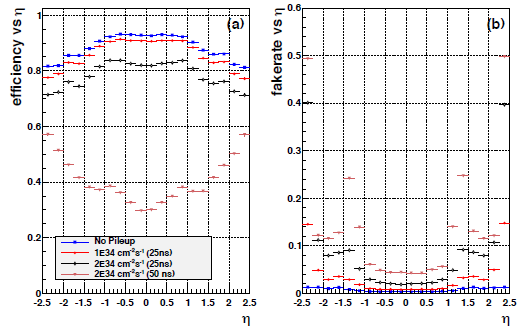
\includegraphics[width=0.9\textwidth]{pixel/reducedperformance2}
%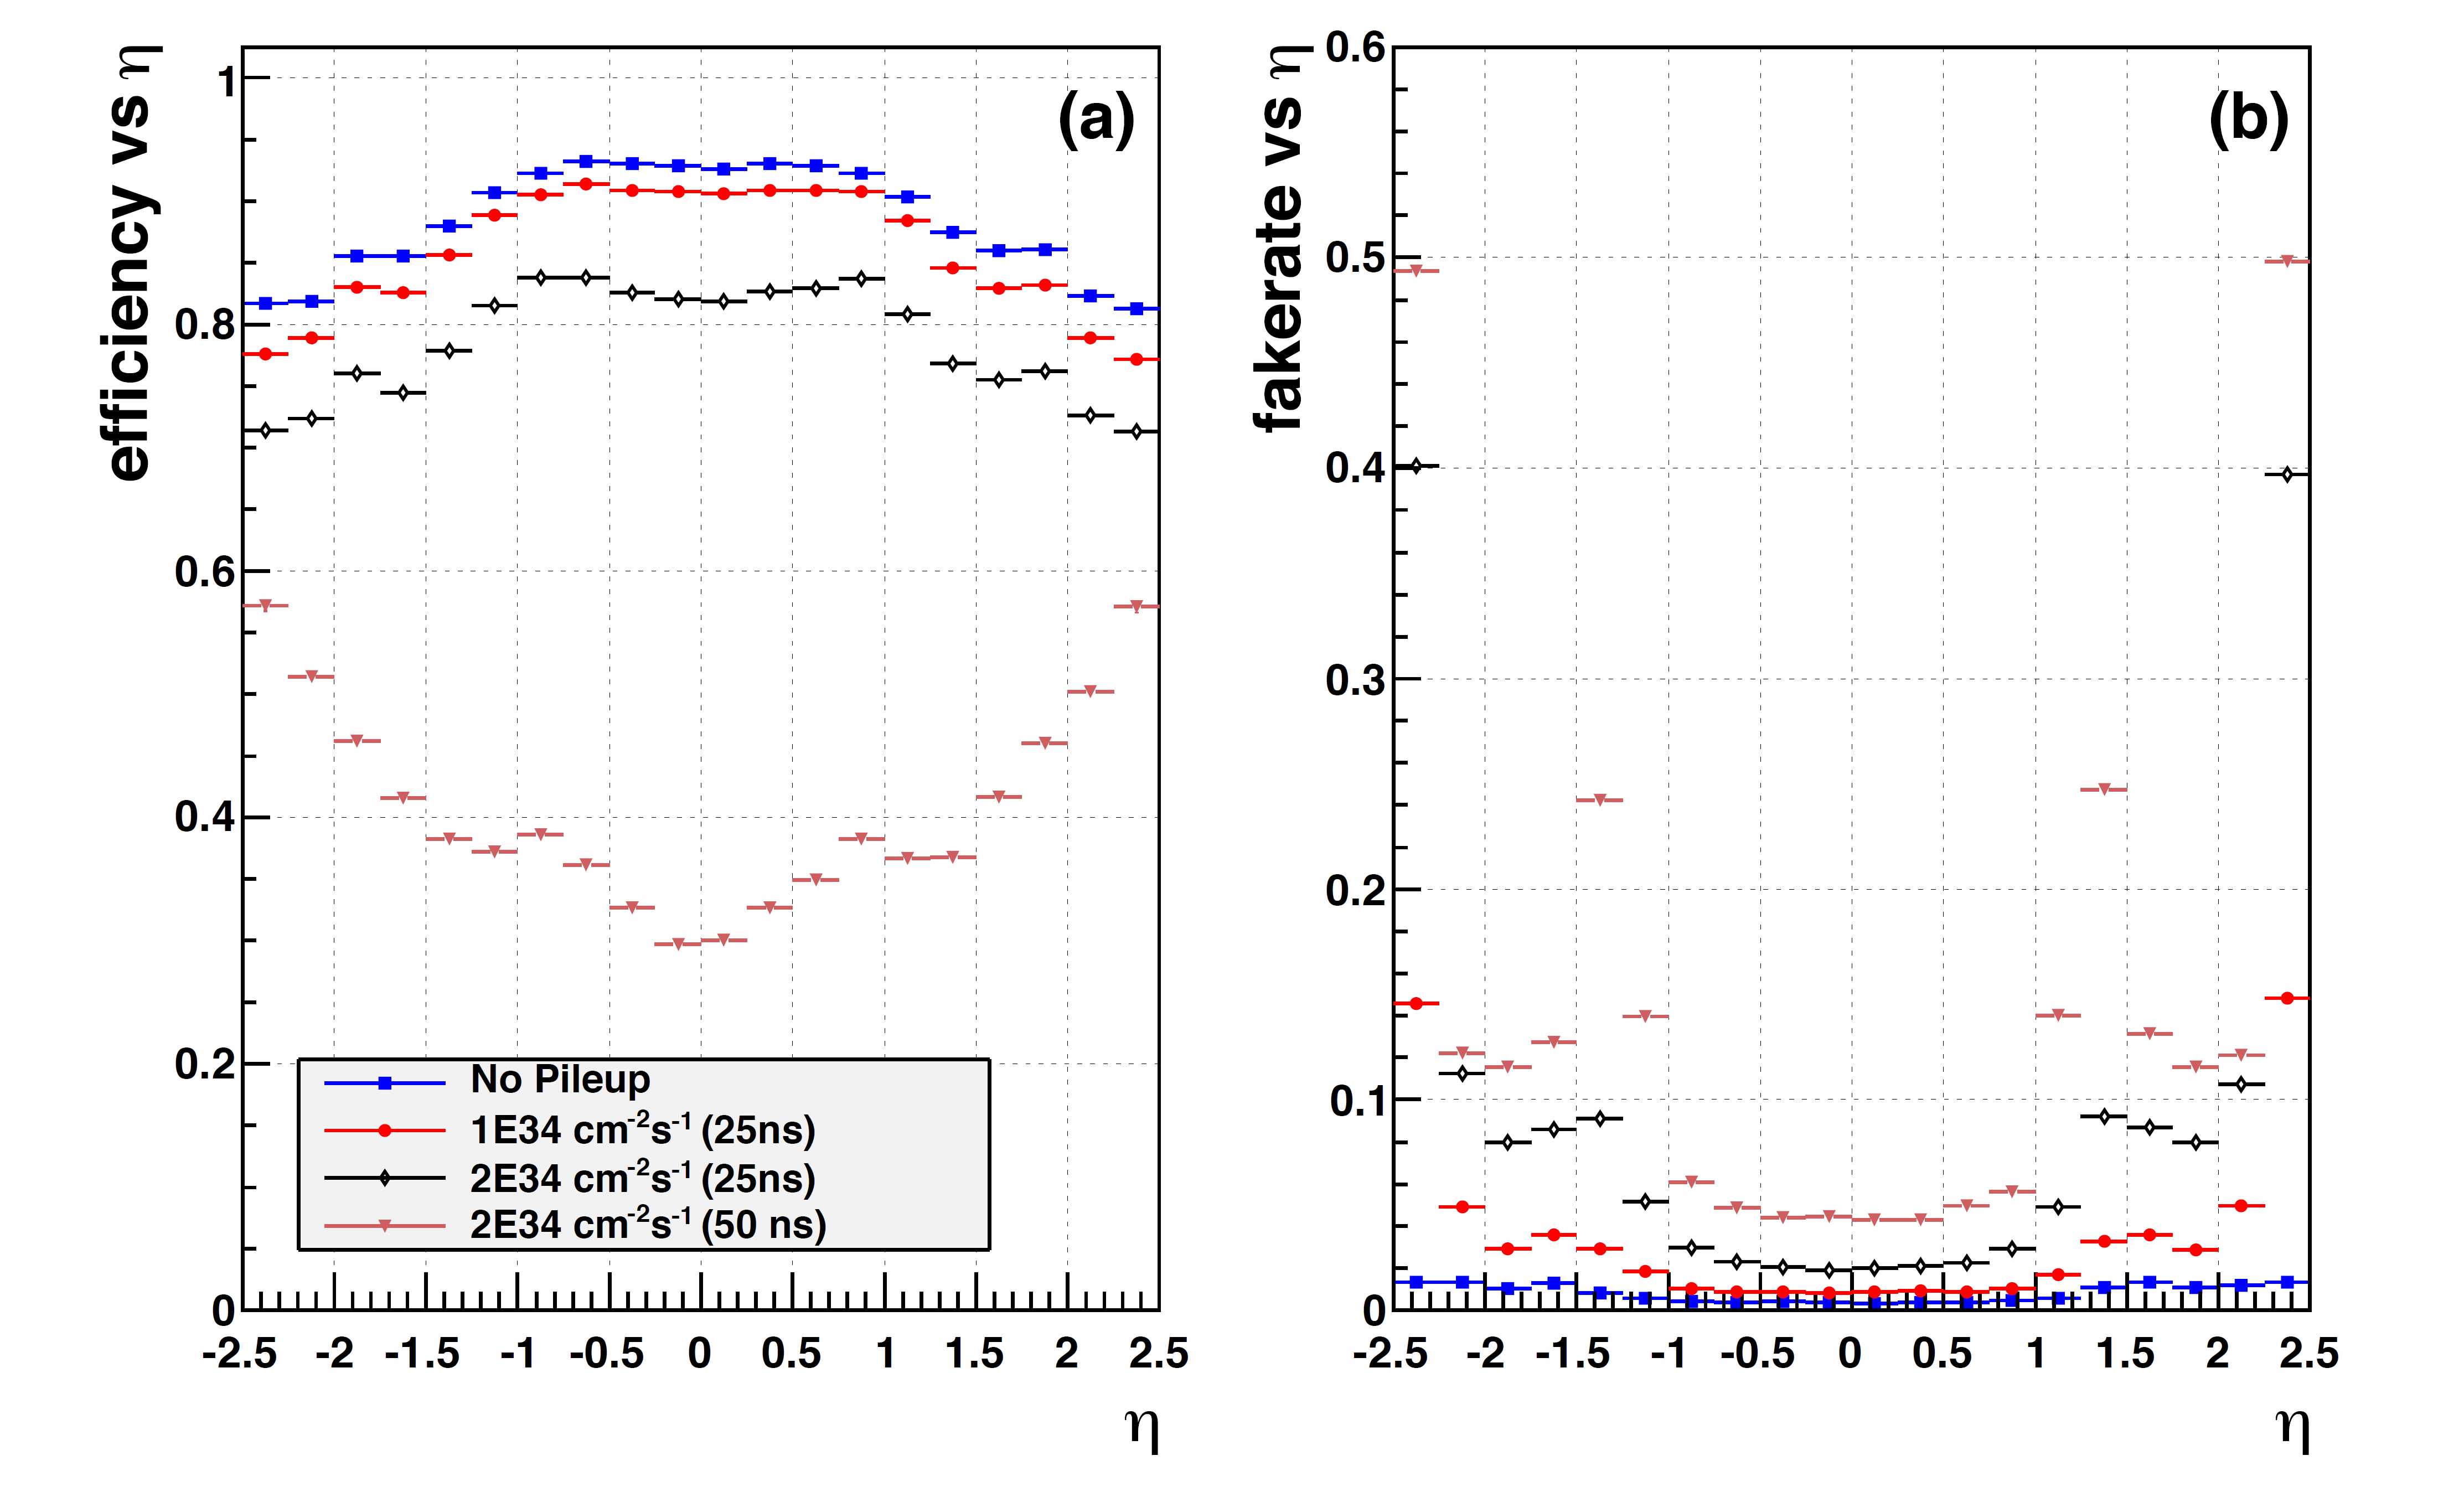
\includegraphics[width=0.9\textwidth]{pixel/reducedperformance}
\caption[Expected performance of the previous pixel detector in simulated \ttbar events.]{Expected performance of the previous pixel detector in simulated \ttbar events: a) efficiency; b) fake rate. Conventions are the same for both plots, considering zero pileup (blue squares), average pileup of 25 (red dots), average pileup of 50 (black diamonds), and average pileup of 100 (magenta triangles).}\label{fig:reduced_performance}
\end{figure}

The present system is designed to offer high performance under these new operational conditions; it is composed of four-layers/three-disks, low mass silicon pixel detectors providing a high performance tracking in the high luminosity environment. The design was leaded by the following requirements\footnote{Taken literally from the technical design report.} 
\bit
\item In running with 50 or more pile-up, maintain the high efficiencies and low fake rates.
\item New pixel readout chip (ROC) to minimize data loss due to latencies and limited buffering in high luminosity running.
\item Minimize degradation due to radiation damage.
\item Optimized detector layout for 4-pixel-hit coverage over the \etac range with minimal innermost layer radius improving pattern recognition and track reconstruction.
\item To reduce material, adopt two-phase $CO_2$ cooling and light-weight mechanical support, moving the electronic boards and connections out of the tracking volume.
\item To reuse the current patch panel and off-detector services, cooling pipes, cables and fibers, adopt DC-DC power converters and higher bandwidth electronics.
\item Reduce number of module types and interfaces simplifying production and maintenance.
\item New smaller diameter beam pipe to accommodate the placement of the inner pixel layer closer to the interaction region.
\eit

The upgraded detector is expected to provide higher efficiencies, lower fake rates, lower dead-time/data-loss, and an extended lifetime of the detector, which translate in better muon ID, b-tagging, photon/electron ID, and tau reconstruction, in both HLT and offline levels. No details about the performance of the current pixel detector are given here since that matter falls beyond the purpose of this document; however, it is documented in Reference\cite{pixel_performance}.

Figure \ref{fig:new_pix} shows the layout of the upgraded pixel detector. The old 3-layer barrel (BPIX), 2-disk endcap (FPIX) system is replaced with a 4-layer barrel, 3-disk endcap system. The additional barrel layer and forward disk provide redundancy for the track pattern recognition and reconstruction.

\begin{figure}[!h]
\centering
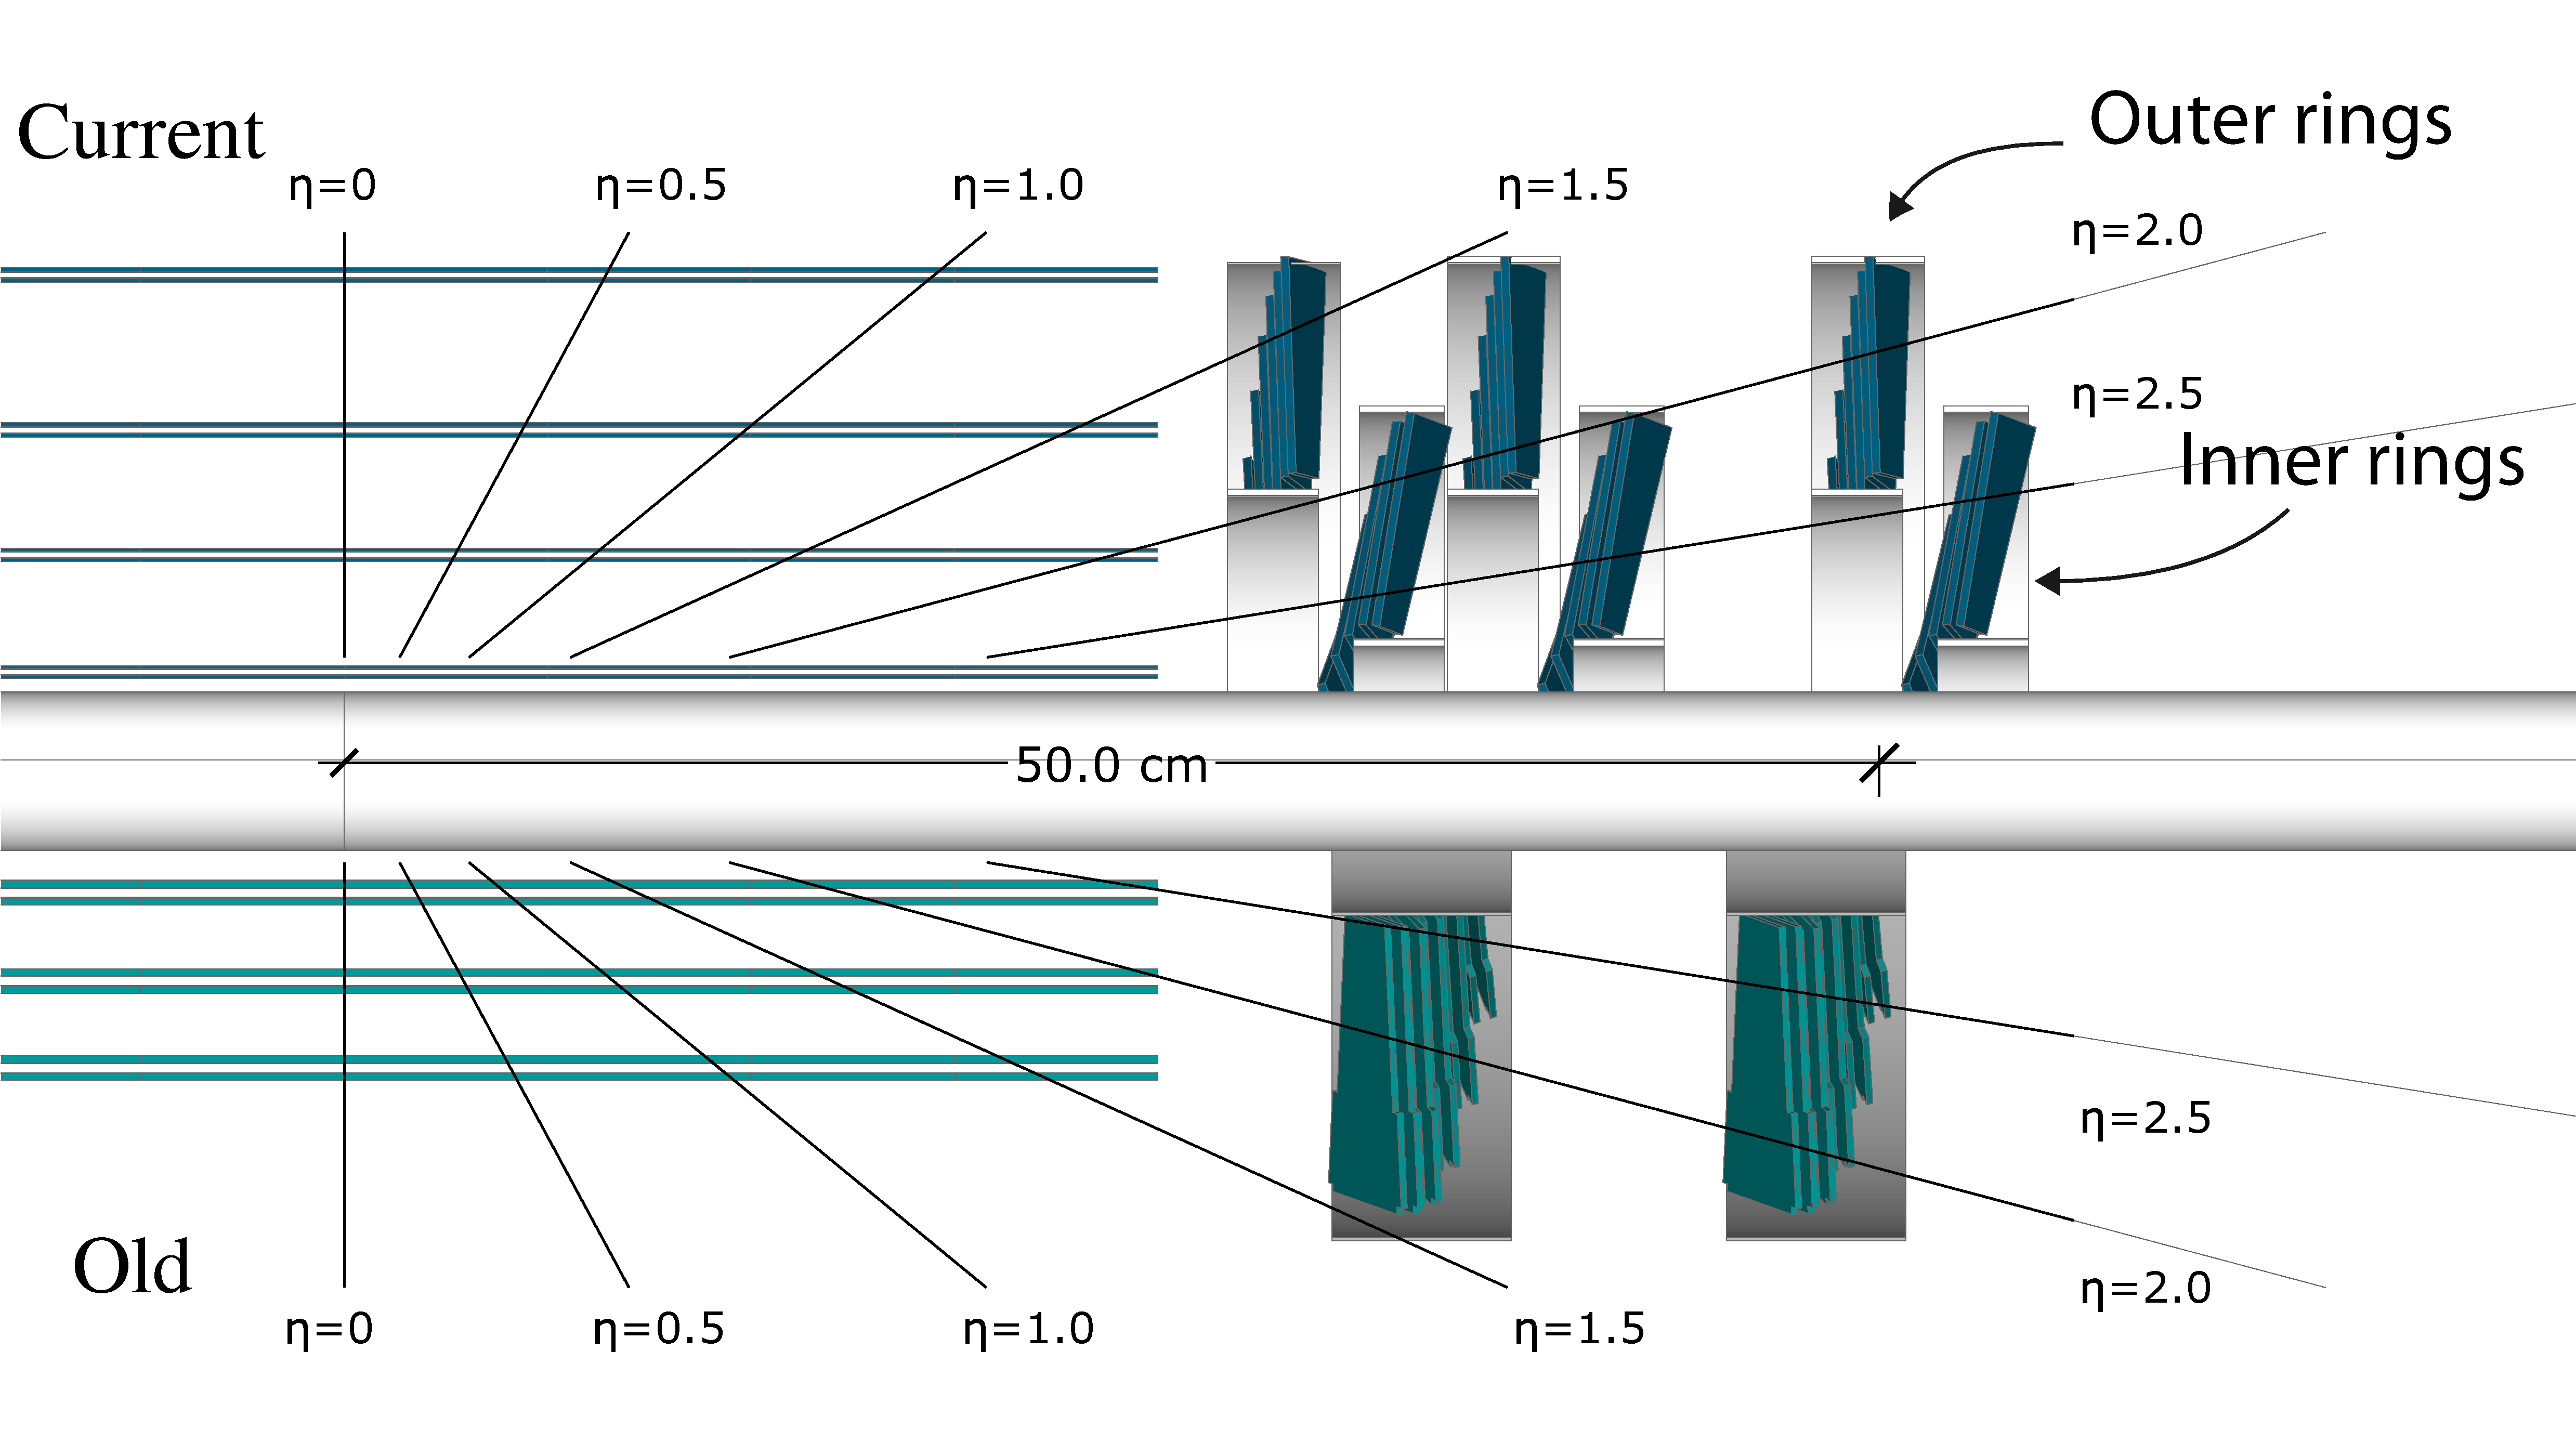
\includegraphics[width=0.6\textwidth]{fpix1.pdf}
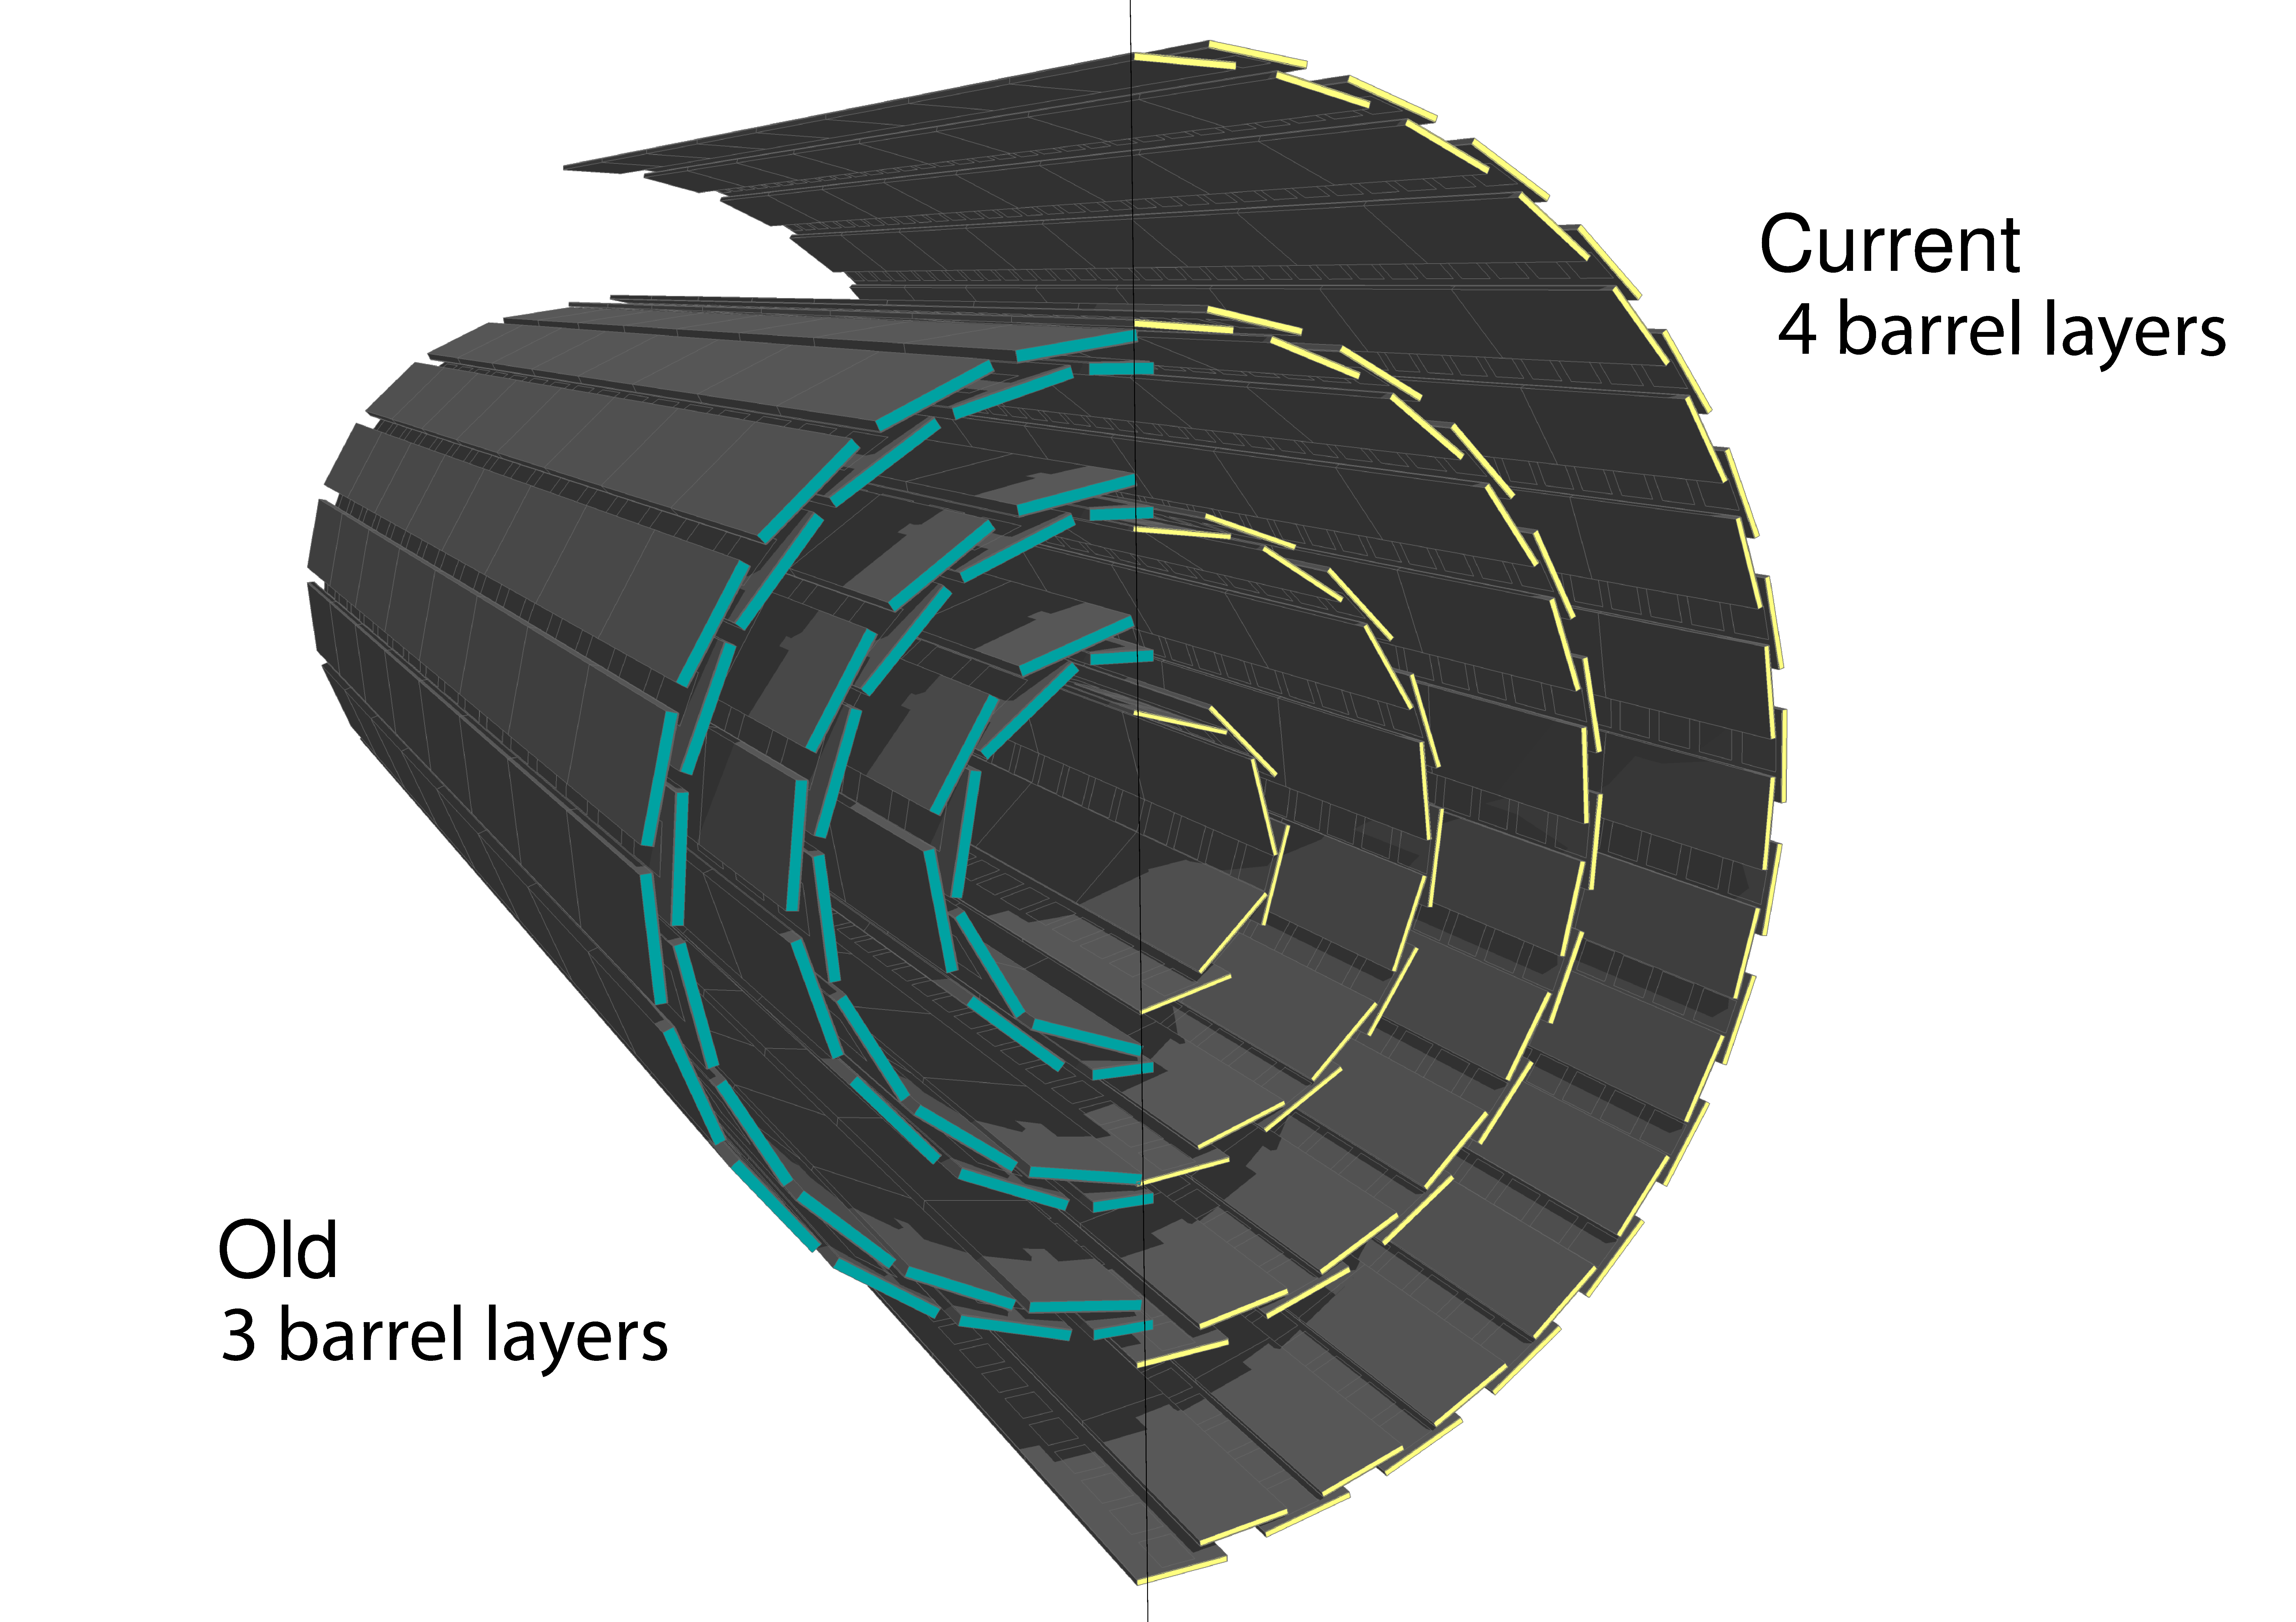
\includegraphics[width=0.39\textwidth]{bpix1.pdf}
\caption[Layout of the upgraded and old pixel detectors.]{Layout and comparison of the layers and disks in the current and old pixel detectors.}\label{fig:new_pix}
\end{figure}

\section{Phase 1 FPix upgrade}

The Phase 1 upgraded FPix system is composed of three disks in each endcap, located at each end of the barrel detector, with a radial coverage ranging from 4.5 to 16.1 cm. The first disk is located along the beam line at 29.1 cm from the IP; the second and third disks are located at 39.6 cm and 51.6 cm from the IP; each disk consists of two half disks. Some of the main features of the upgraded FPix System are:
\bit
\item Pixel size: $100 \times 150$ $\mu$m 
\item Only one type of modules: 2x8 ROC modules
\item Modules oriented radially to improve resolution in $r-\phi$.
\item Minimize the gap in 4-hit coverage between the end of the 4th-barrel layer and the forward-most disk.
\item All three identical disks on each side of the IP.
\eit

Figure \ref{fig:fpix_layout} shows a schematic structure of the FPix half disk; each half disk is composed of two sections, inner and outer, where the pixel modules are assembled.

\begin{figure}[!h]
  \centering
  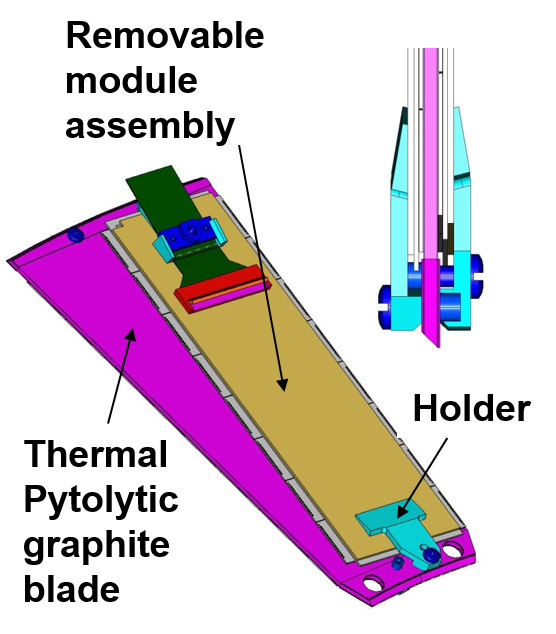
\includegraphics[width=0.32\textwidth]{pixel/module1}
  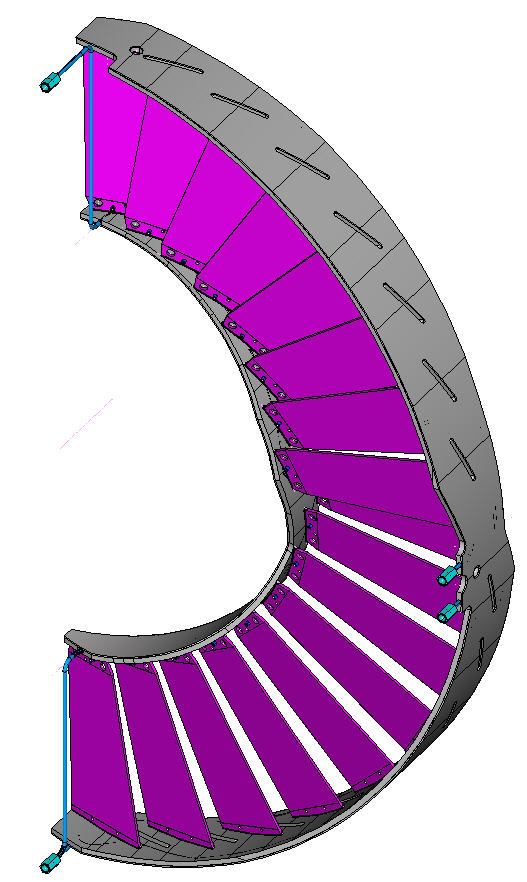
\includegraphics[width=0.32\textwidth]{pixel/half_disk_inner}
  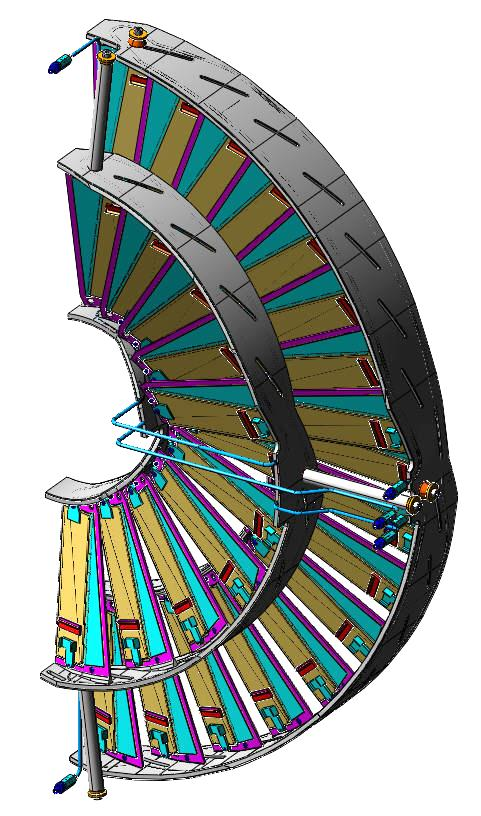
\includegraphics[width=0.32\textwidth]{pixel/half_disk}
\caption[FPix half disk design.]{FPix half disk design; FPix module (left) mounted on a blade, outer half disk (center), assembled half disk (right).}\label{fig:fpix_layout}
\end{figure}

In total, there are 56 modules (896 ROCs) per half-disk, 34 modules in the outer ring and 22 modules in the inner ring. The pixel modules are attached to the blades by a pair of module holders. Modules are designed to be removable and replaceable without disassembling the half-disks; thus those modules that suffer failure or degradation can be easily replaced during an annual technical stop.

Blades on the outer assembly are rotated by 20$^o$ forming a turbine-like geometry; in addition, they are arranged in an inverted cone array with the blades tilted by 12$^o$ with respect to the IP in order to guarantee excellent resolution in both the azimuthal and radial directions throughout the FPIX acceptance angle for the inner assembly.

\section{FPix module structure}

\begin{figure}[!h]
  \centering
  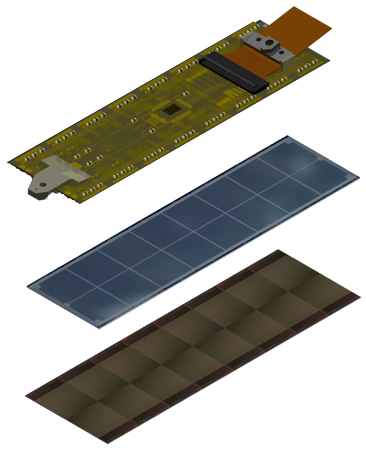
\includegraphics[width=0.33\textwidth]{pixel/fpix_structure1}
  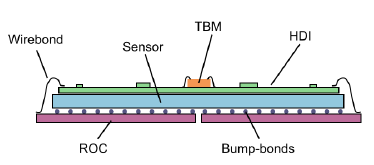
\includegraphics[width=0.63\textwidth]{pixel/fpix_structure2}
  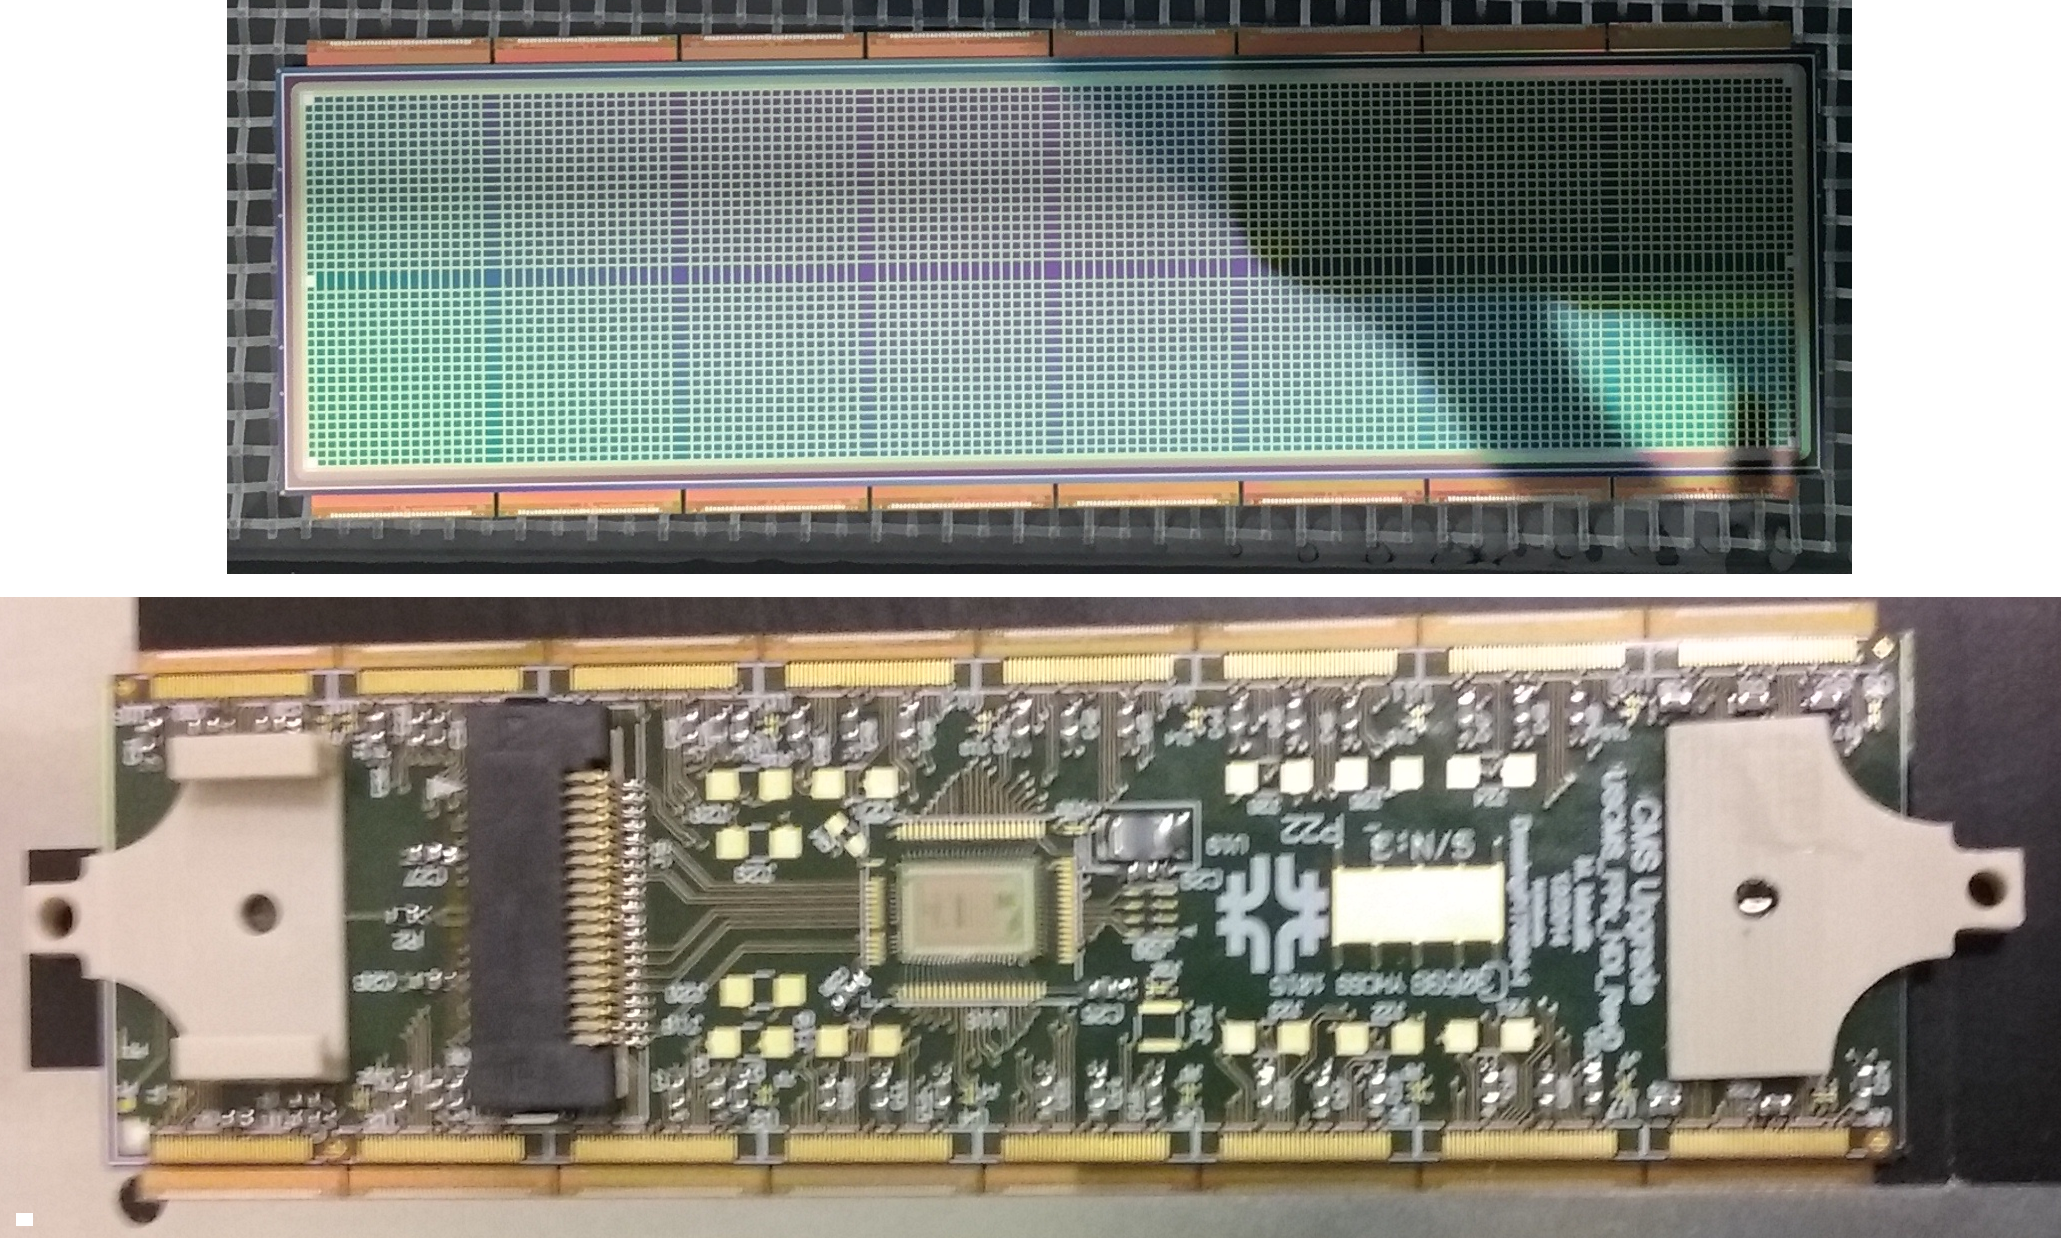
\includegraphics[width=0.63\textwidth]{pixel/bbm_hdi}
  \caption[FPix module structure.]{Top: FPix module structure; The bare silicon sensor is bump-bonded to the ROCs to form the BBM; then the HDI is glued on top of the BBM and wirebonded to the ROCs. Bottom: pictures of actual BBM and HDI.}\label{fig:fpix_struc}
\end{figure}

The current CMS pixel detector is composed of 1184 pixel modules in the BPIX sector with a total 79 million of pixels; the FPix sector contains 672 with approximately 45 million of pixels. Figure \ref{fig:fpix_struc} shows an schematic view of the FPix modules structure. The n$^{+}$-in-n \ti{Silicon sensor} is Bump-Bonded to the 16 ROC to form the detector unit known as \ti{Bump-Bonded Module} (BBM) with 66560 pixels. The \ti{High Density Interconnect} (HDI) is glued on top of the BBM and wirebonded to the ROCs to provide them the required signals and power. The modules are attached to the support structure using the end holders glued to the HDI.

\section{FPix module assembly}

The construction of the modules for the current FPix system was divided between two sites located at Purdue University and UNL; testing facilities were located at University of Kansas and Fermi National Accelerator Laboratory (Fermilab). The integration facility was based at Fermilab. 

The BBM was prepared by a commercial vendor, while the HDI was populated at Fermilab, with all the electronic components like resistors, capacitors and the central component known as \ti{Token Bit Manager} (TBM) which is in charge of managing the information coming from the silicon sensors and going to the ROCs. Both BBM and HDI were sent to the assembly sites ready to be glued together.  


\begin{figure}[!h]
  \centering
  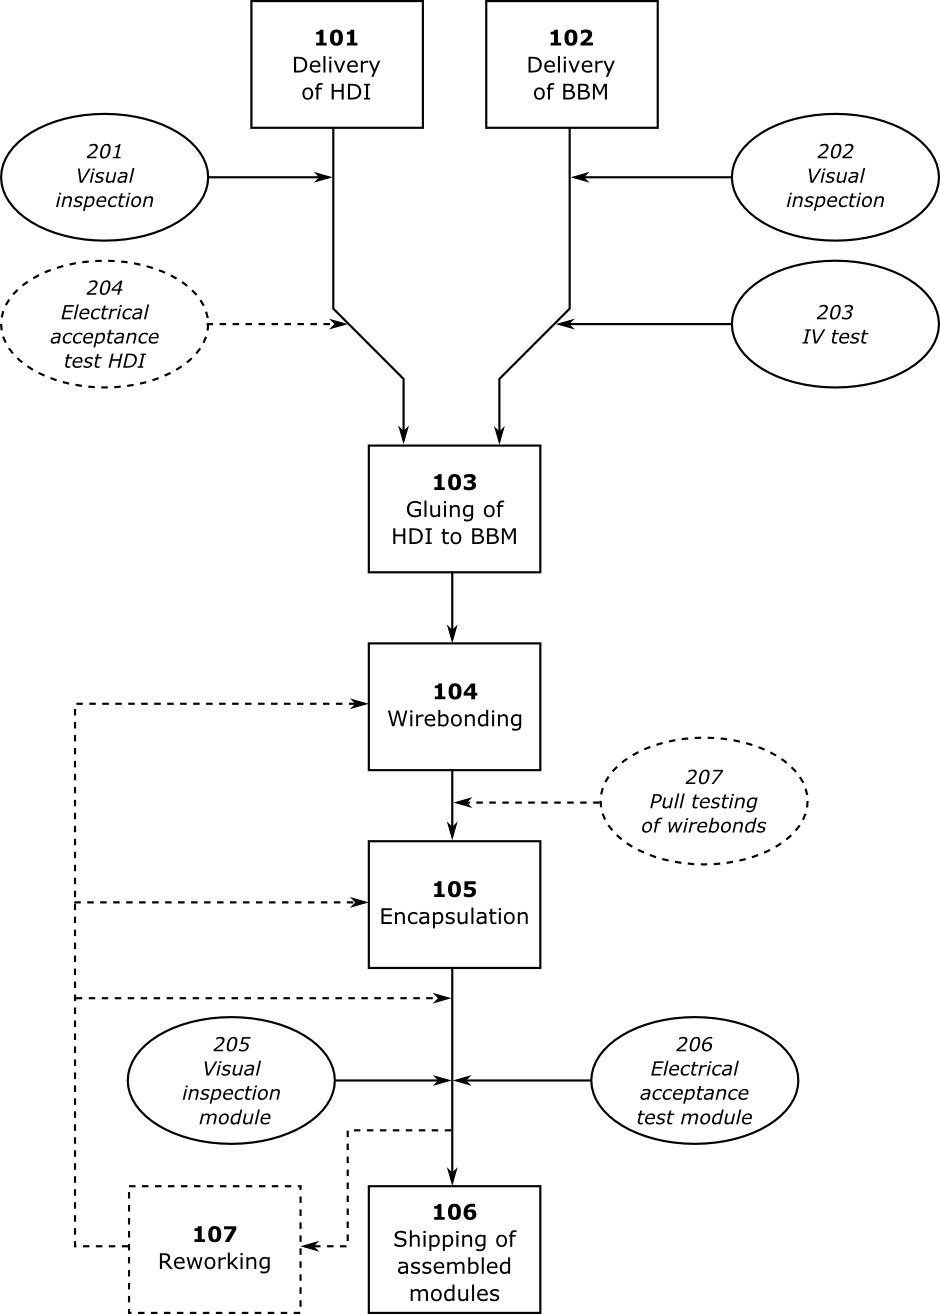
\includegraphics[width=0.7\textwidth]{pixel/UNLworkflow}
  \caption[UNL module assembly work flow.]{UNL module assembly work flow. Dashed lines represent occasional quality testing and reworking procedures; 10X numbers represent the stage within the assembly procedure while 20X numbers represent testing stages along the assembly procedure.}\label{fig:unlworkflow}
\end{figure}


The module production procedure was designed following a production line structure. Figure \ref{fig:unlworkflow} shows the work flow followed at the UNL assembly site. Once the BBM and HDI arrive, they are submitted to visual inspection looking for defects, scratches, dents or short circuits. Modules passing the visual inspection are tested for electrical acceptance and performance. BBM and HDI are then glued employing robotic pick-and-place machines that integrate optic tools, pattern recognition algorithms, and glue dispensing; the semi-automated gluing process improves the uniformity of the technique. After 10 hours of curing, glued modules are moved to the wirebonding station where ROCs and HDI are electrically connected employing semi-automated ultrasonic wirebongding machines; occasionally, some of the wires are pull tested for quality control. After this step, modules are fully functional, hence, a basic functionallity test is done at a subset of modules to control the manufacturing process.    

In the next stage, the wirebonds are encapsulated with an elastomeric compound (\ti{Sylguard}) in order to protect them against mechanical damage and electrical shorts; the encapsulation process is performed employing the robotic pick-and-place machine which also integrates the encapsulant dispensing system. Once the encapsulation ends, modules are mounted on module holders and submitted to a head cycle to cure the sylguard.    

The module assembly sites were also responsible for the testing and characterization of the assembled pixel modules. That testing included, visual inspection, electrical acceptance, performance testing under controlled temperature conditions that simulate the expected operational conditions; in case of any necessary reworking, the modules were returned to the appropriate stage.

In the final stage, the assembled and tested modules were shipped to University of Kansas for further characterization.  

Each stage in the assembly procedure is documented with an ~\ti{Standard Operating Procedure} (SOP) document that describes the procedures to be followed by the operator. The full set of SOPs can be found in Reference \cite{unl_sop}.     

In the following sections a detailed description of the gluing and encapsulation stages will be presented. The full set of tools was designed by Dr. Frank Meier Aeschbacher. 

\subsection{Pick and place machine setup}

Figure \ref{fig:setup} shows the full setup used to perform the gluing and encapsulation steps. The gantry used in the setup is a custom made \ti{AGS15000 Series Gantry}, fabricated by Aerotech \cite{aerotech}, which offers translational motion in 3D ensuring coverage of any position in the work field; in addition, rotational motion is provided in the \ti{gantry head} in the usual x-y plane (gantry table plane).

\begin{figure}[!h]
  \centering
  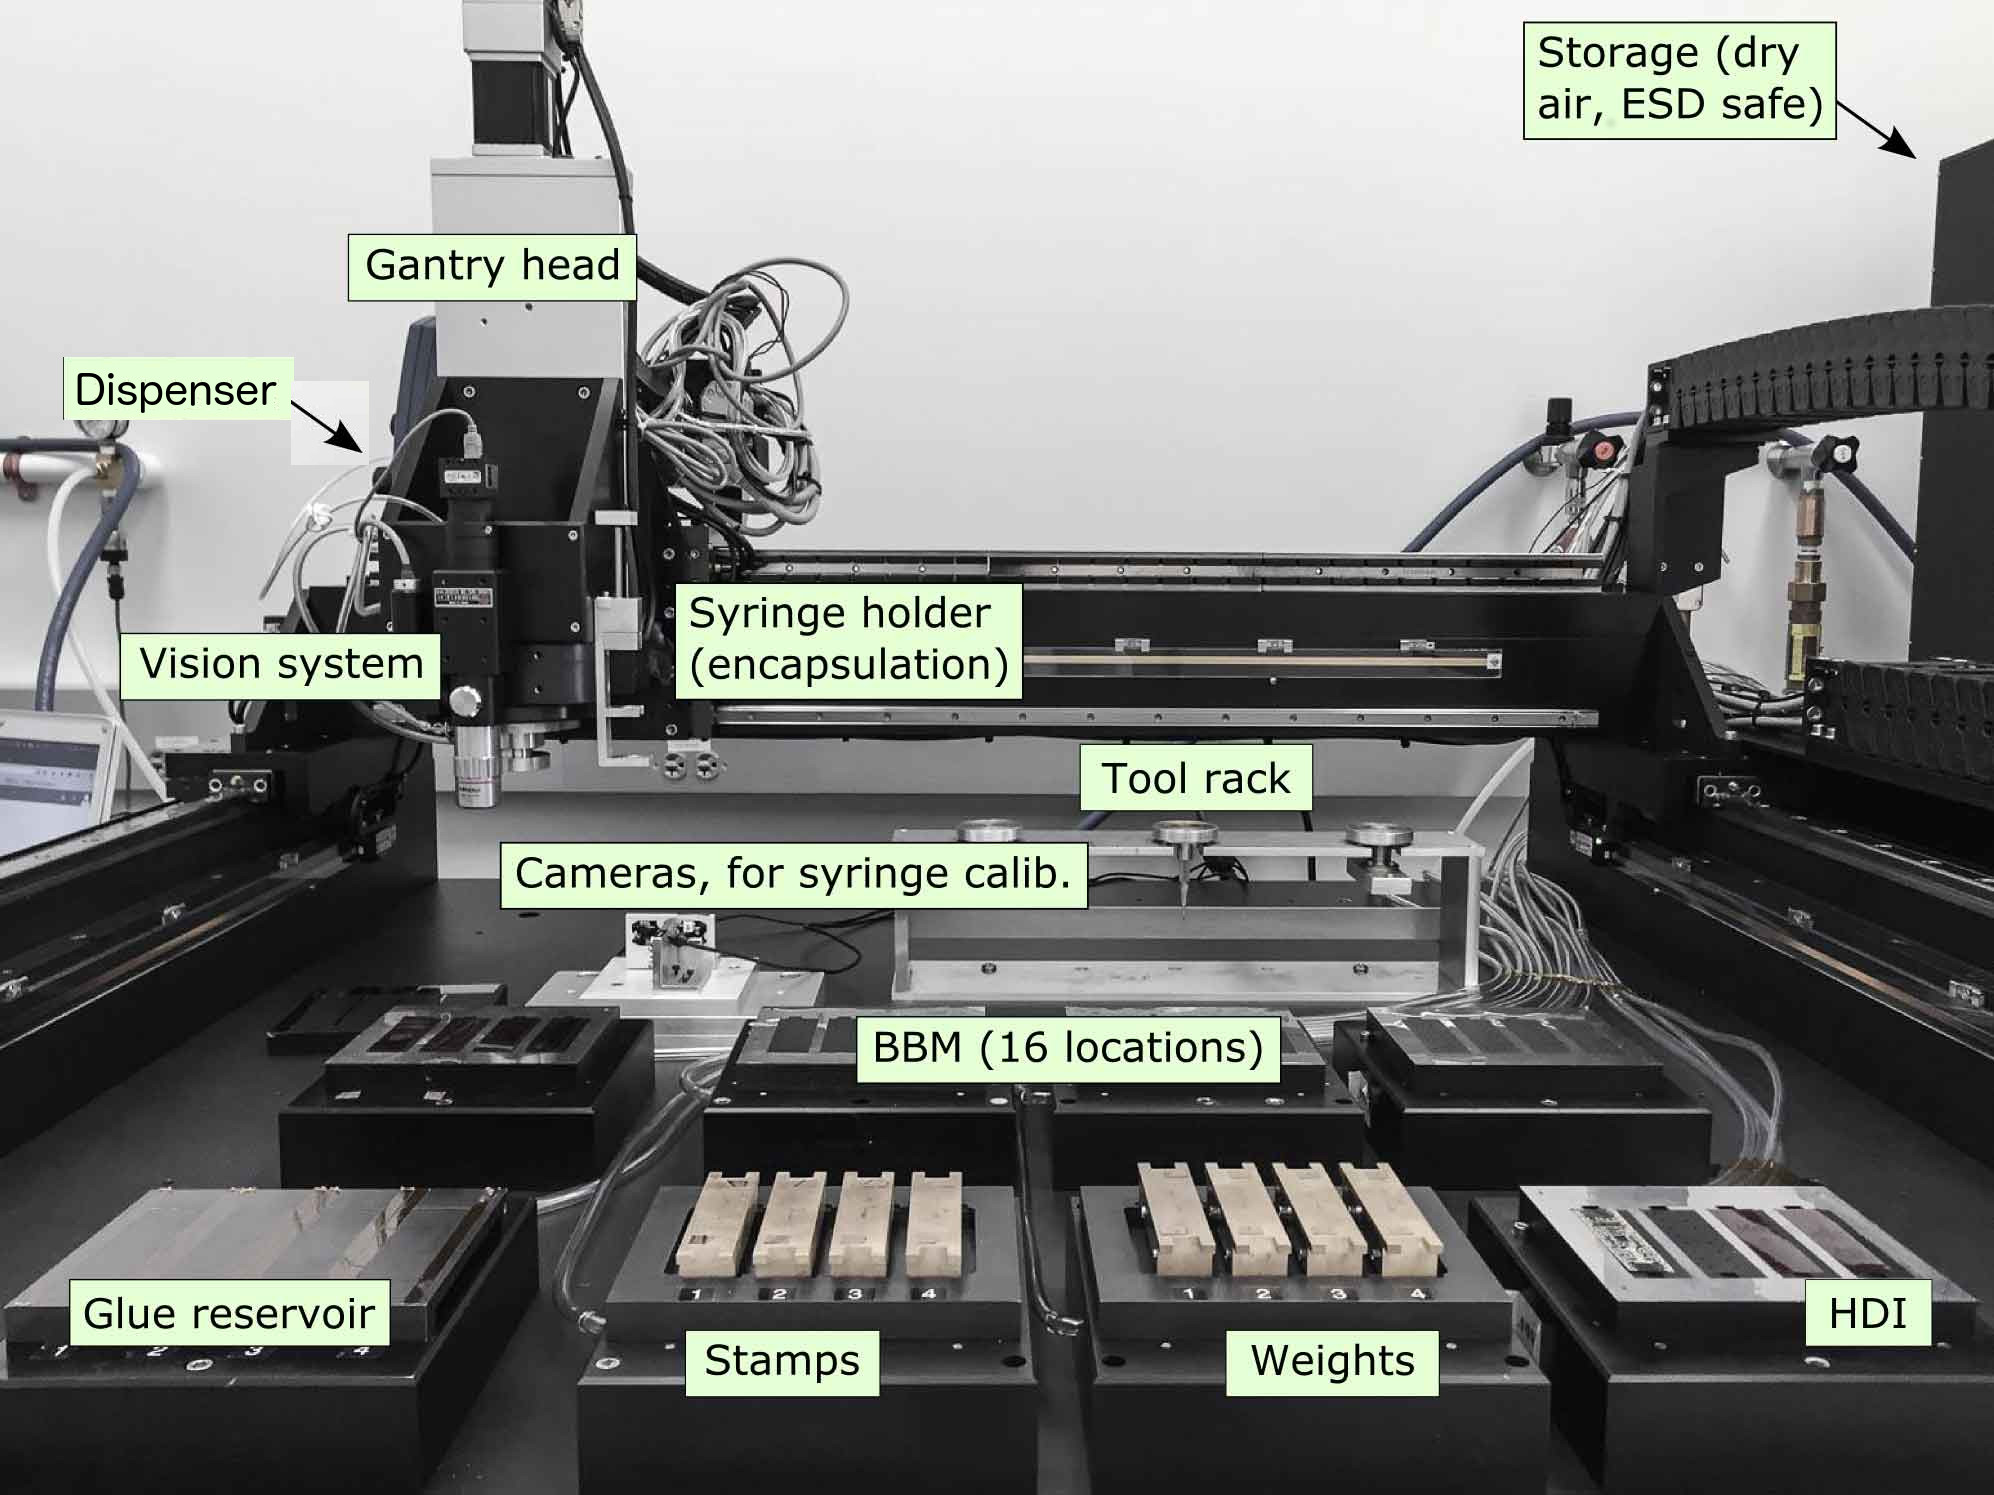
\includegraphics[width=\textwidth]{pixel/gantryFull16labeled}
  \caption[Full gluing and encapsulation setup]{Full gluing and encapsulation setup. }\label{fig:setup}
\end{figure}

A set of eight hard-anodized aluminum chucks, composed of a \ti{base chuck} and a \ti{plate chuck} each, henceforth chuck and plate respectively, were designed to house the parts and tools needed along the gluing process; Figure \ref{fig:chuck} shows the details of a chuck.      

\begin{figure}[!h]
  \centering
  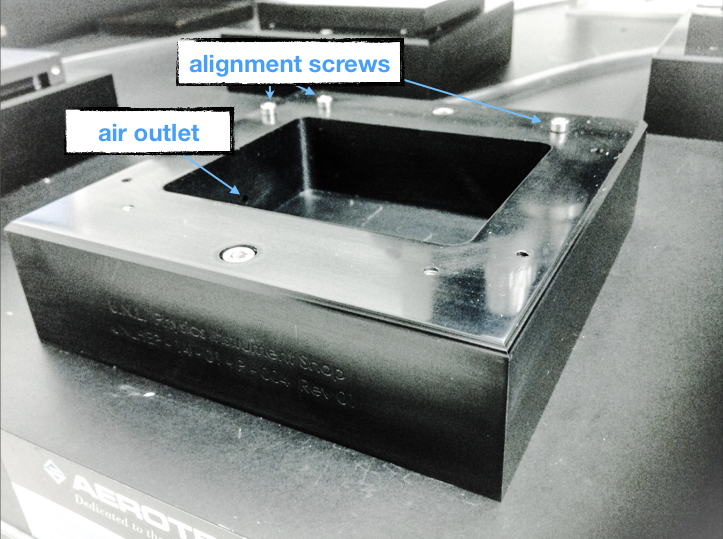
\includegraphics[width=0.48\textwidth]{pixel/chuck}
  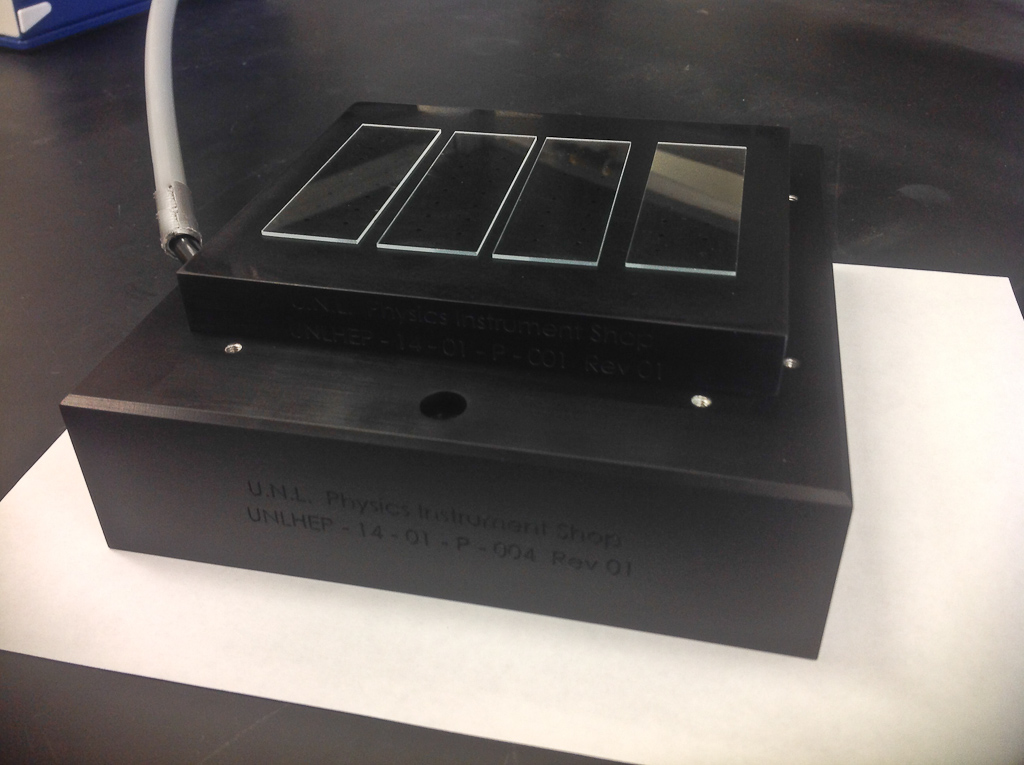
\includegraphics[width=0.48\textwidth]{pixel/chucksAnodized}
  \caption[Bare and full chucks]{Left: Chuck detailed internal view. Right: full chuck housing glass slides. The vacuum connection is visible on the left.}\label{fig:chuck}
\end{figure}

Each chuck is connected to an independent vacuum line such that the plate is hold fixed; both pieces are polished to seal the vacuum with no use of O-rings. The three screws serves as references for aligning the plates with the chucks. There are four types of plates; HDI/BBM plate, the glue reservoir plate, stamp plate, weight plate.

\subsubsection*{Chucks}

Four chucks are used to accommodate sixteen BBMs (four per plate); the holes in the BBM/HDI plate (see Figure \ref{fig:bbm_hdi_plates}) are intended to hold the BBM/HDI safely fixed to the plate by the action of the vacuum, while the stencil (100 $\mu$m in thickness) allows for a very accurate positioning of the BBM/HDI; it is thin enough so that the alignment is controlled by the edges of the ROC and no force is applied to the sensor.     

\begin{figure}[!h]
  \centering
  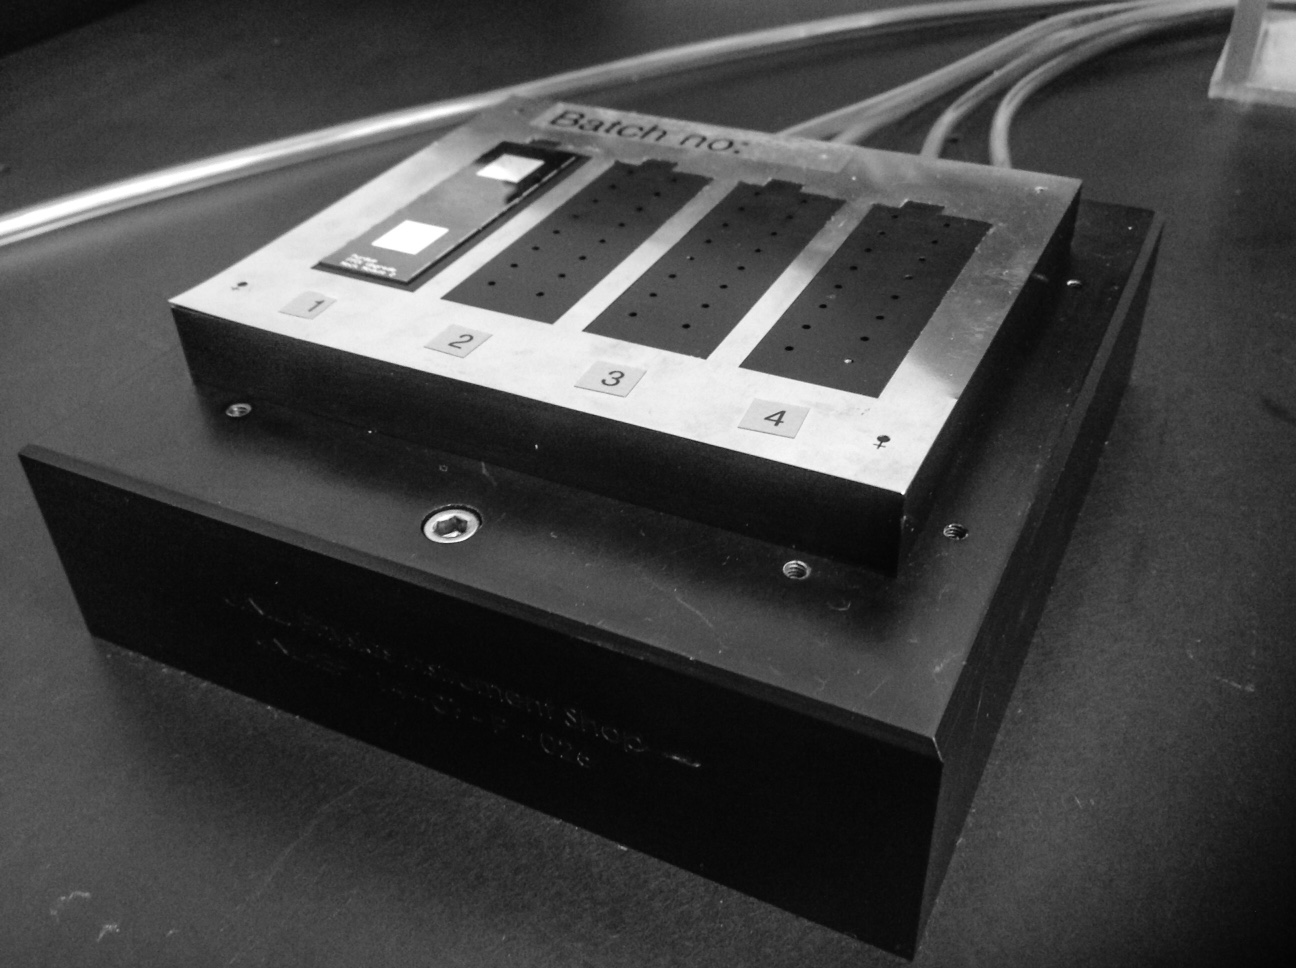
\includegraphics[width=0.32\textwidth, height= 0.32\textwidth]{pixel/bbm_chuck}
  \includegraphics[width=0.32\textwidth, height= 0.32\textwidth]{pixel/hdi_plate_adj}
  \includegraphics[width=0.32\textwidth, height= 0.32\textwidth]{pixel/hdi_stencil}
  \caption[BBM/HDI plate]{Left: BBM/HDI plate with a mock module that reproduce the BBM features. Center: the pockets in the top and bottom sides accommodate the module holders. Right: bare HDI and BBM showing the alignment provided by the stencil.}\label{fig:bbm_hdi_plates}
\end{figure}

One chuck is dedicated to accommodate four HDIs. Although BBM/HDI plates have the same design, the HDI chuck have four independent pockets instead of only a big one, in order to enable the release of one HDI at a time; hence, it is connected to 4 vacuum lines. That is not required for the BBMs because they are no moved from their original location. An additional adjustment was made to the HDI plate in response to the HDI back surface which is not totally flat but has irregularities; these irregularities caused vacuum leaks that were addressed by adding a kapton tape layer to the HDI plate, as shown in the center of Figure~\ref{fig:bbm_hdi_plates}. The tracks ensure the vacuum action and the tape flexibility ensures the sealing.    

One chucks holds the \ti{glue reservoir} plate, as shown in Figure \ref{fig:glue_reservoir}. Each of the four reservoirs is a pocket just 100 $\mu$m deep, suitable for retaining sufficient glue to be applied to the BBM.  

\begin{figure}[!h]
  \centering
  %\includegraphics[width=0.4\textwidth, height= 0.4\textwidth]{pixel/glue_plate_adj}
  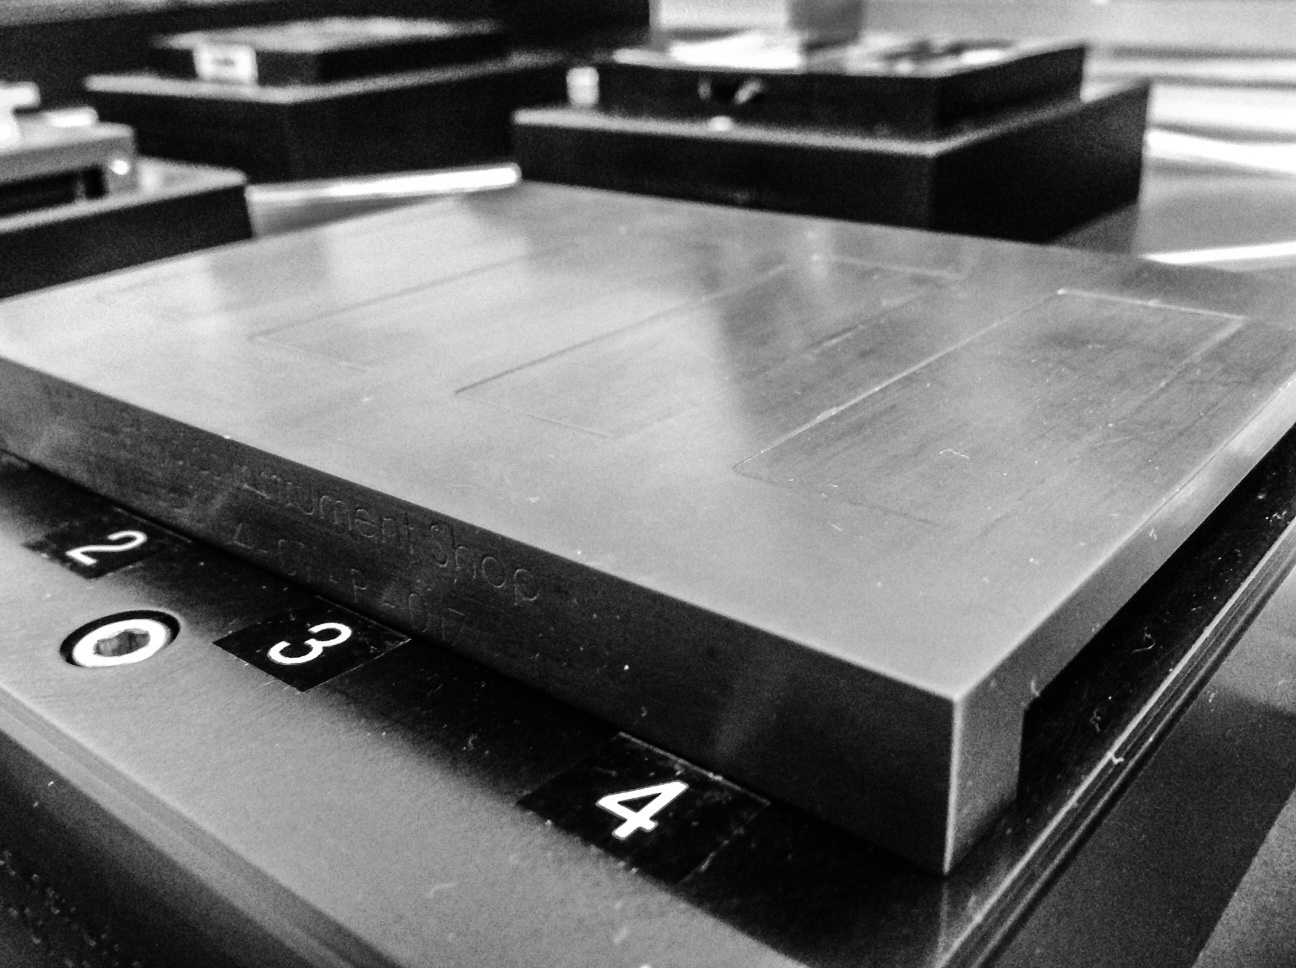
\includegraphics[width=0.5\textwidth]{pixel/glue_reservoir}
  \caption[Glue reservoir plate]{Glue reservoir plate. The four pockets are 100 $\mu$m deep. }\label{fig:glue_reservoir}
\end{figure}

The remaining two chucks house the \ti{stamp plate} and the \ti{weight plate} which in turn house the \ti{stamp tools} and the \ti{weight tools} as shown in Figure~\ref{fig:st_wt_plates}. 

\begin{figure}[!h]
  \centering
  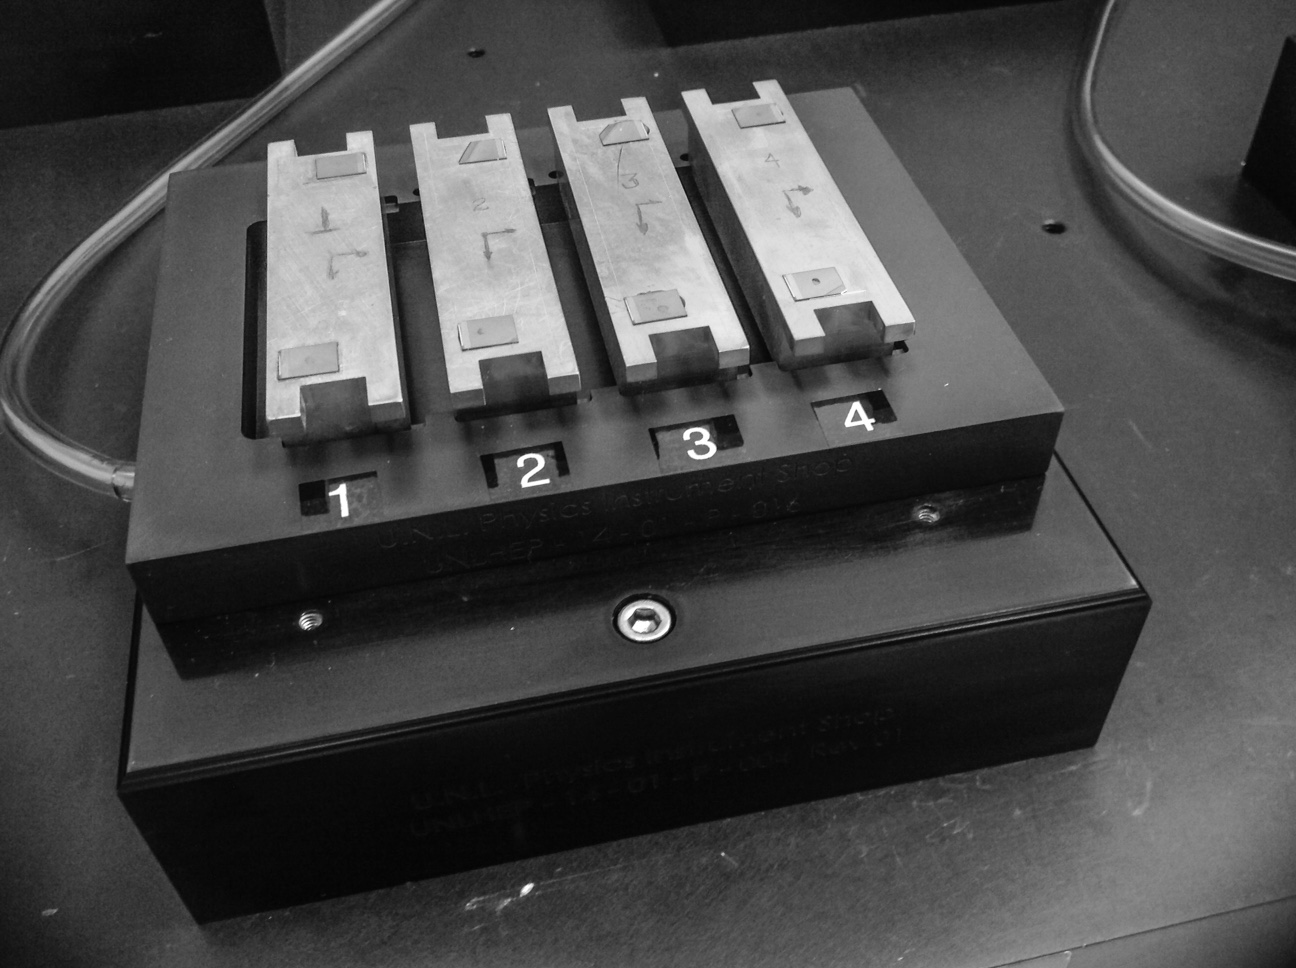
\includegraphics[width=0.45\textwidth]{pixel/chuck_stamps}
  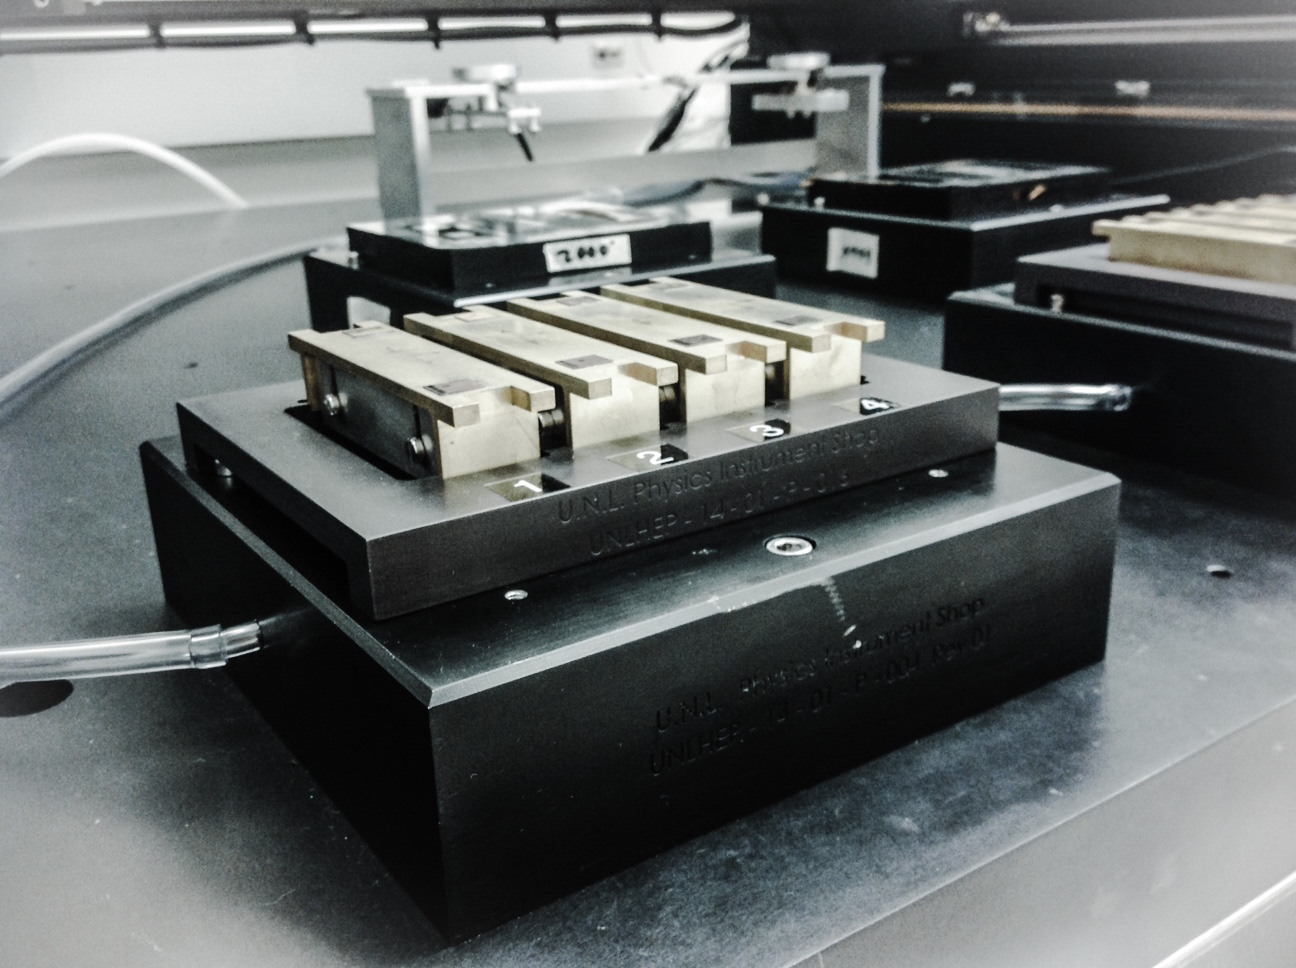
\includegraphics[width=0.45\textwidth]{pixel/chuck_weights}
  \caption[Stamp and Weight tools in chucks]{Chucks housing stamp tools(left) and weight tools(right).}\label{fig:st_wt_plates}
\end{figure}

\subsubsection*{Stamp and weight tools}

\begin{figure}[!h]
  \centering
  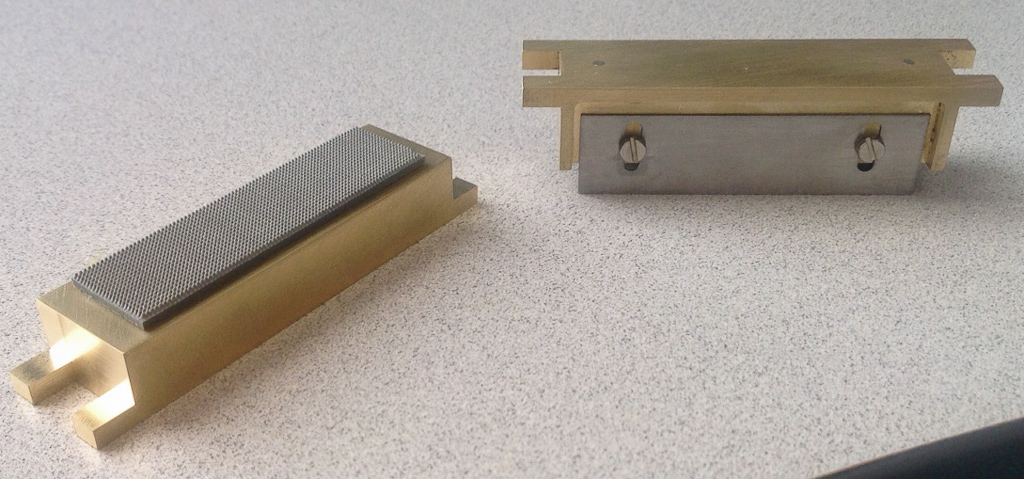
\includegraphics[width=0.45\textwidth, height=0.35\textwidth]{pixel/tools}
  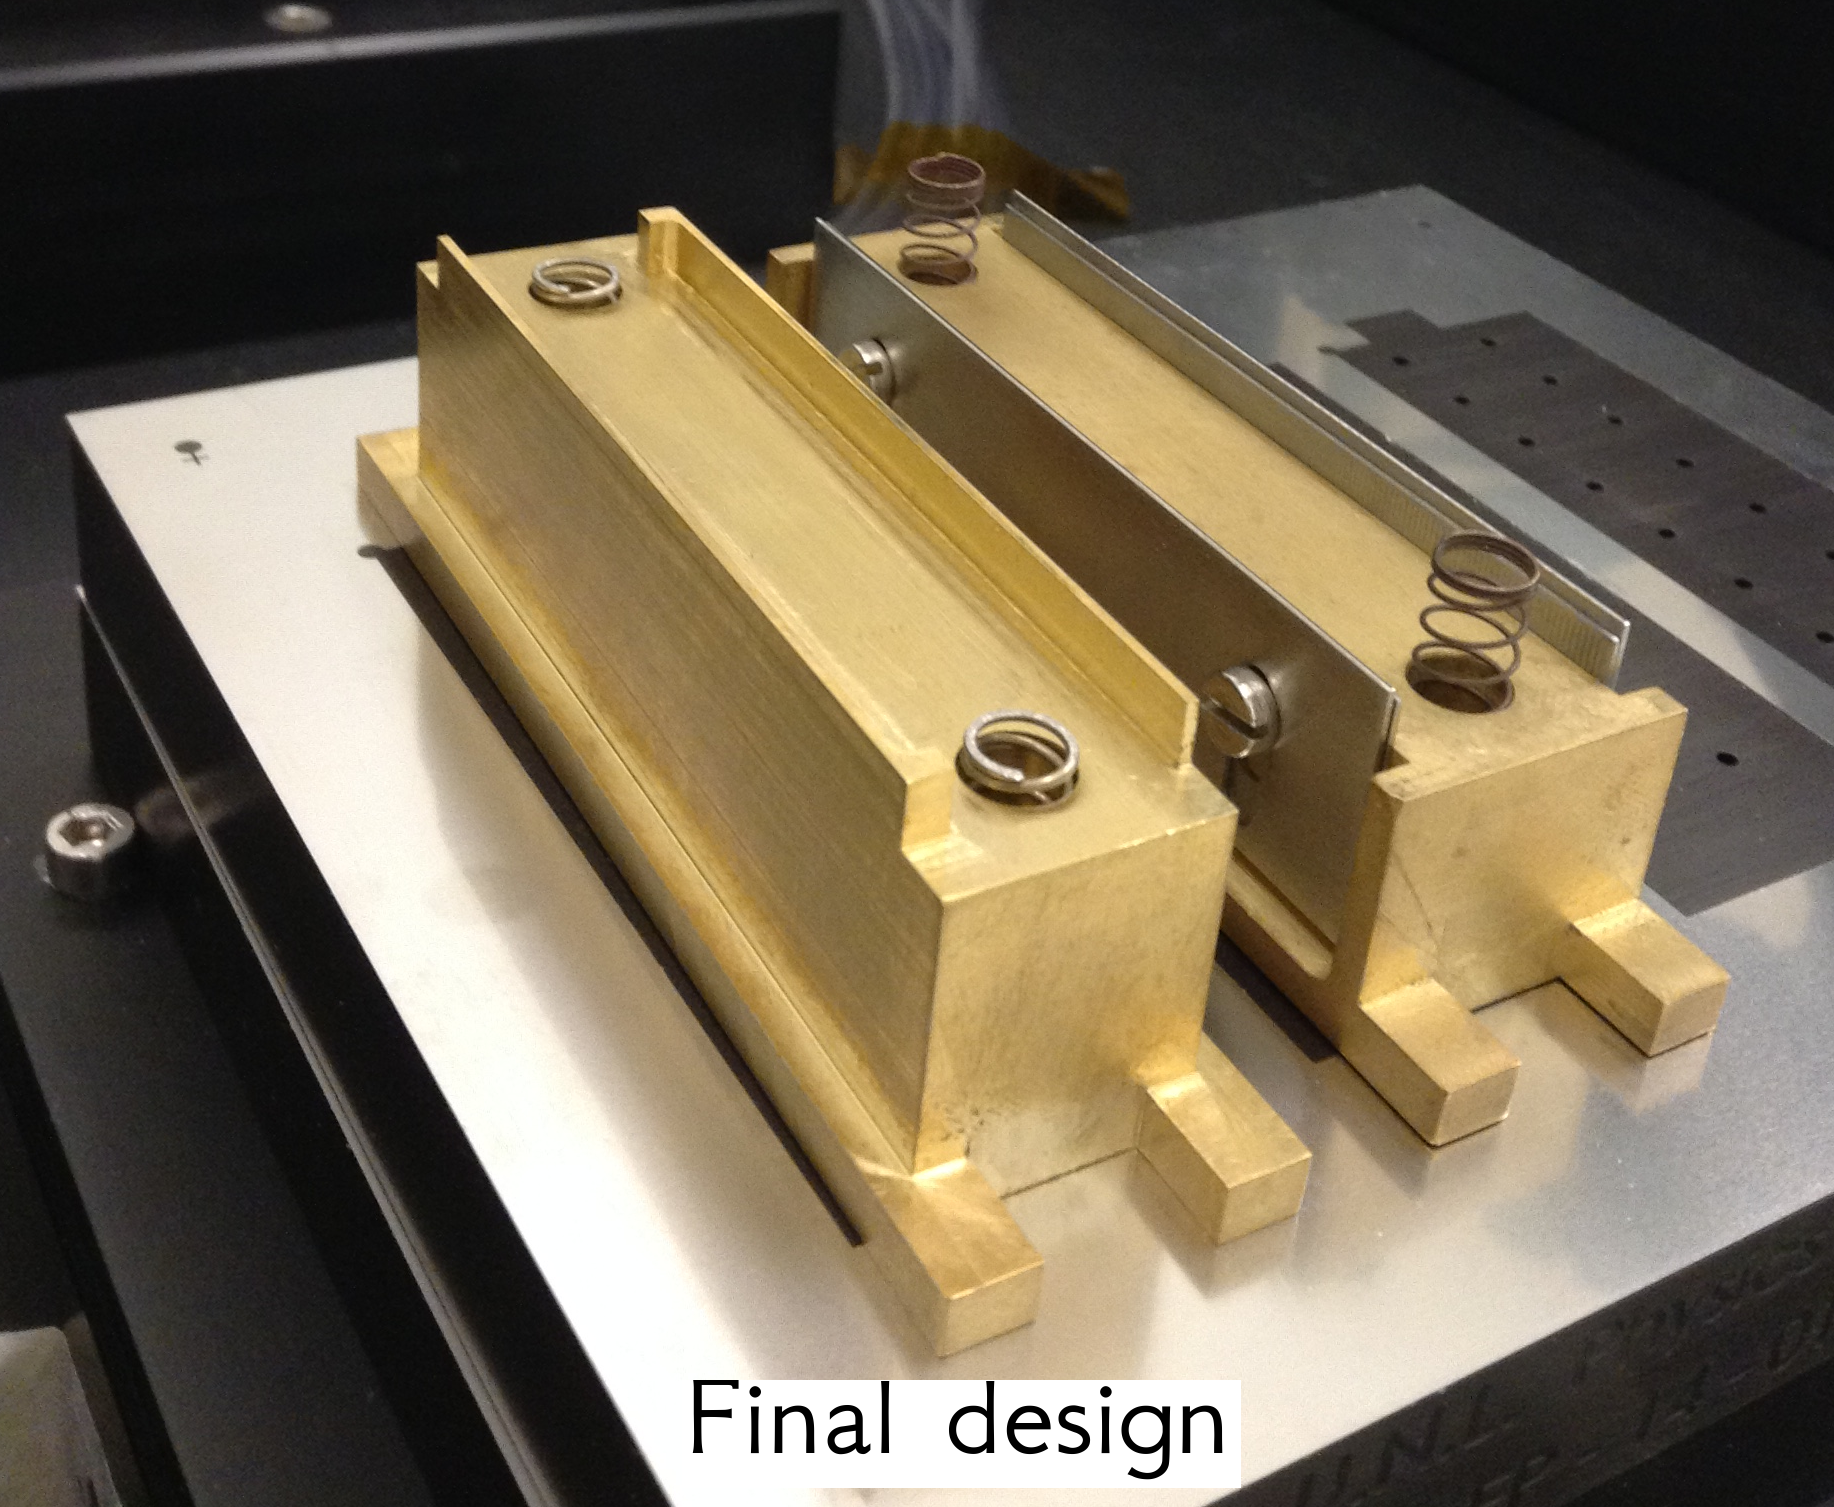
\includegraphics[width=0.45\textwidth, height=0.35\textwidth]{pixel/tools2}
  \caption[Stamp and Weight tools]{Stamp and weight tools. Both tools are made of brass; the stamp tool includes a rubber stamp while the weight tool includes four stainless steel blades to apply force while curing. The final weight tool design eliminates the blades (right).}\label{fig:st_wt}
\end{figure}

Stamp and weight tools are a set of custom made tools, all produced by the UNL Physics department machine shop (see Figure~\ref{fig:st_wt}). The very first design of the weight tool included four stainless steel blades and two springs; the blades matched the rows of 8 ROC bond pads on the HDI to apply force while curing. The springs apply force to the module end holders on the HDI. The final design of the tool eliminates the issues associated to the alignment of the blades, by integrating them into the design in the form of narrow blade-like brass edges. The weight tools are made with 260 g of brass.      

The stamp tool is composed of a brass piece of 200 g and a rubber stamp piece attached to the bottom side of the brass piece; it is used to pick the glue from the glue reservoir and then stamp it over the BBM. An extensive testing process was performed in order to determine the most appropriate features of the gluing strategy. Figure~\ref{fig:stamp_pattern} shows the four stamp patterns tested and a picture of the first two attached to the stamp tools; the variations of the stamp pattern design were based on the results from testing for:

\begin{figure}[!h]
  \centering  
  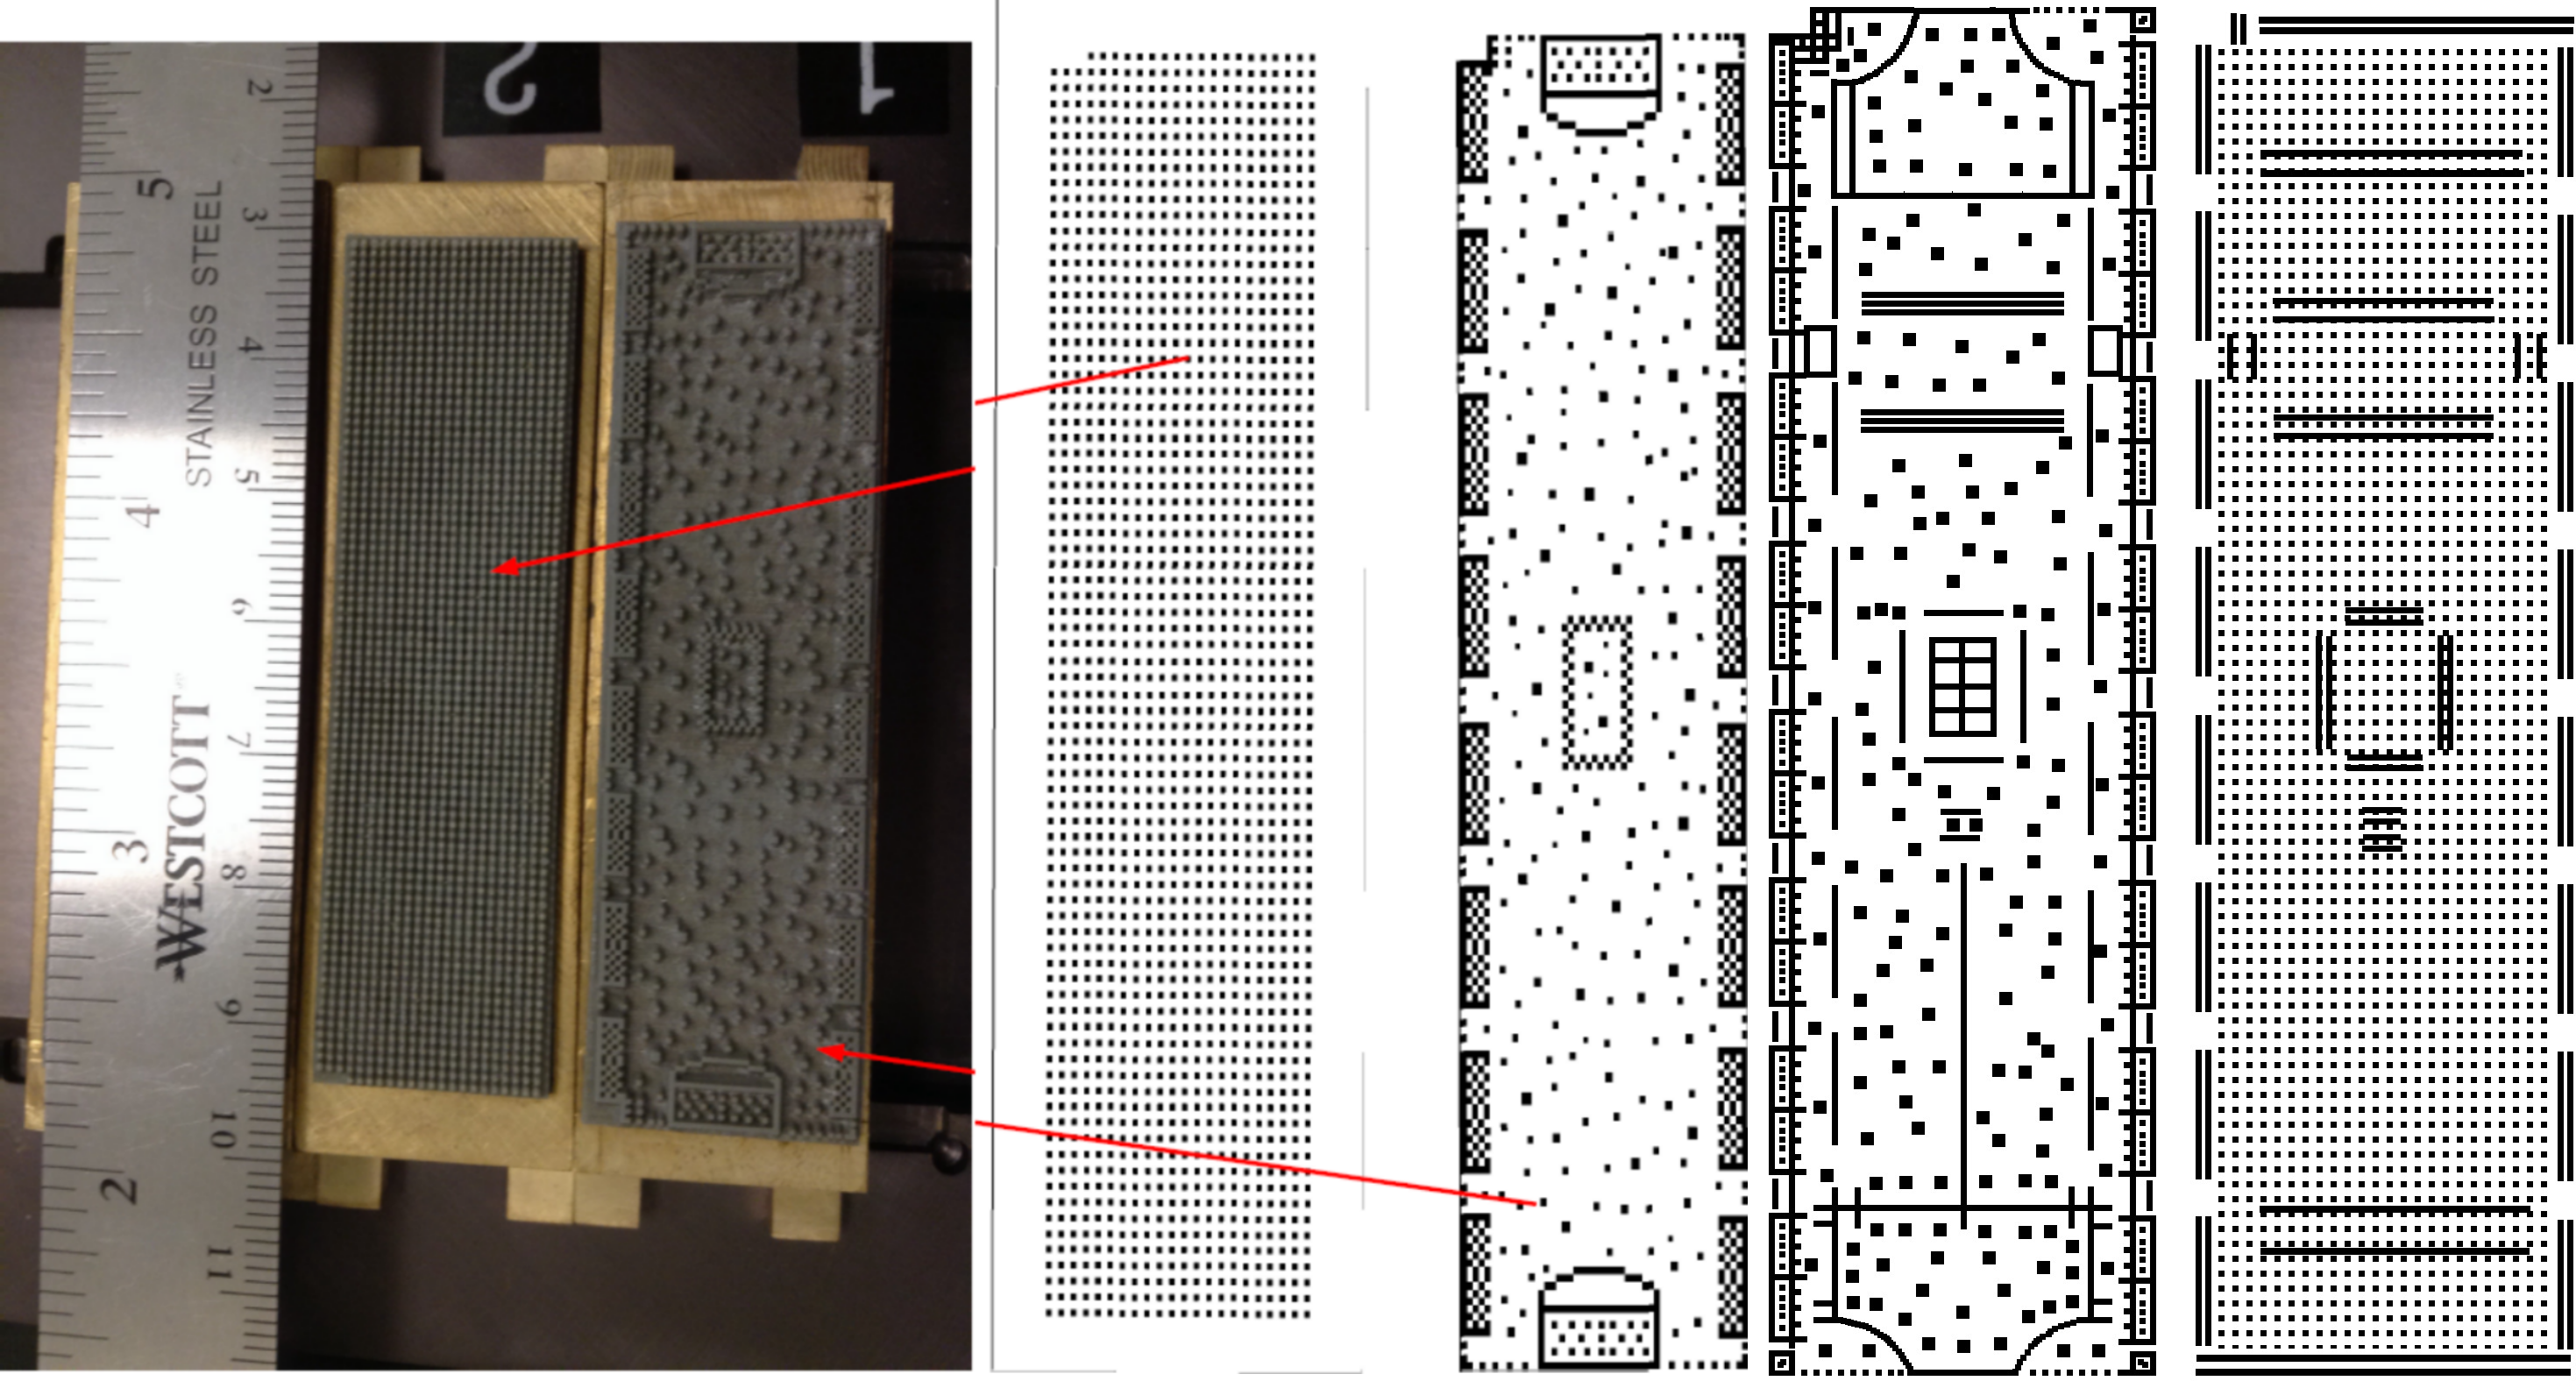
\includegraphics[width=0.8\textwidth]{pixel/stamps} 
  \caption[Stamp patterns]{Stamp patterns evaluated along the glue testing process; the picture on the left show the first two versions mounted on the stamp tool while the final version is on the right.}\label{fig:stamp_pattern}
\end{figure}

\bit
  \begin{figure}[!h]
  \centering
  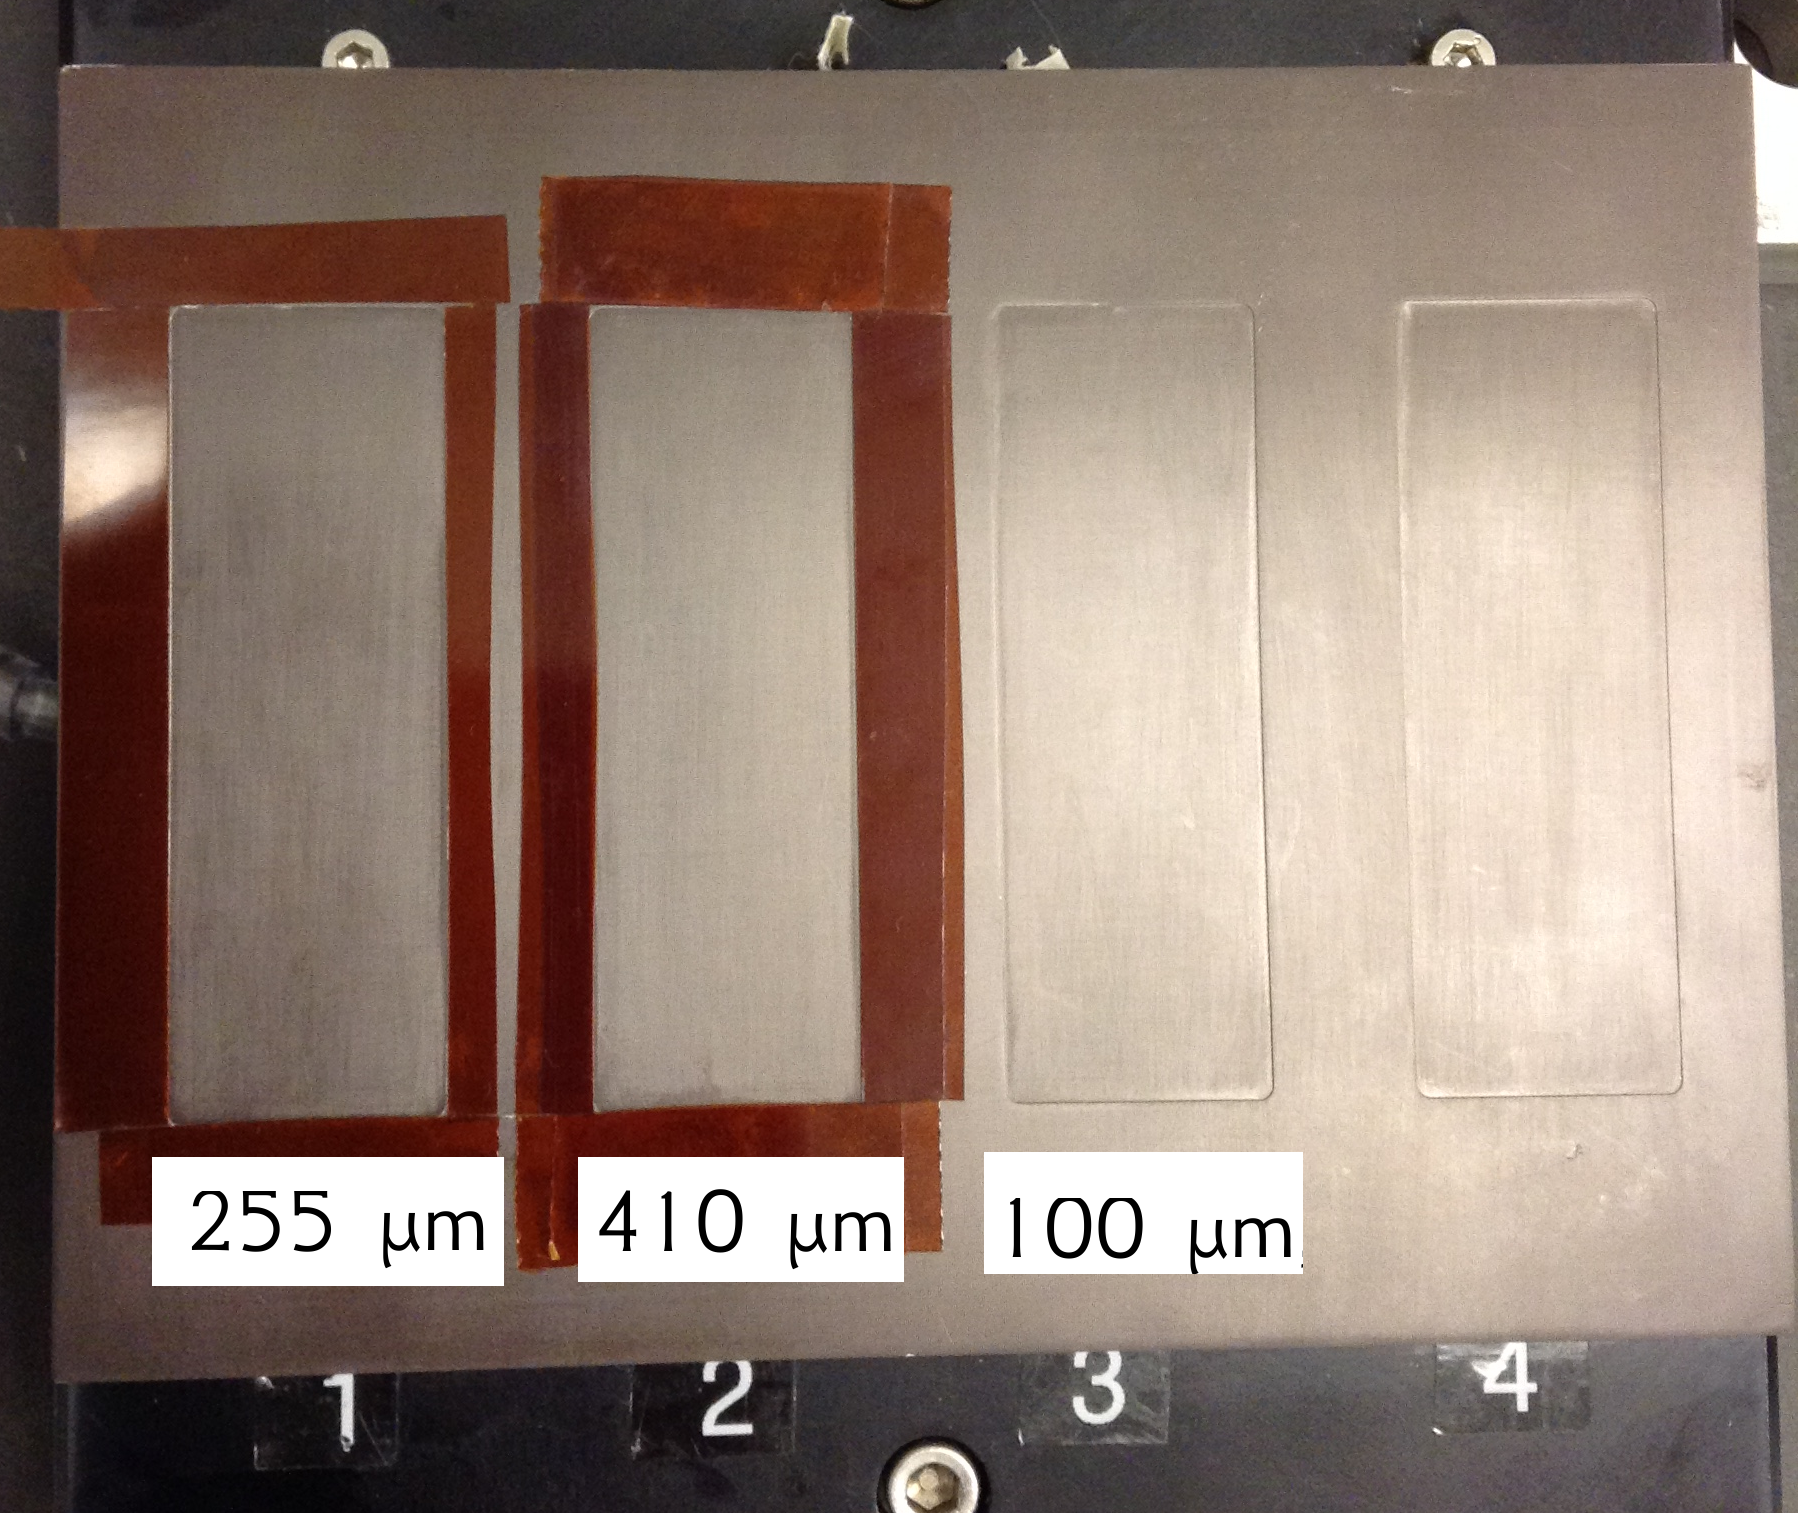
\includegraphics[width=0.4\textwidth, height=0.4\textwidth]{pixel/reservoir_depth_test}
  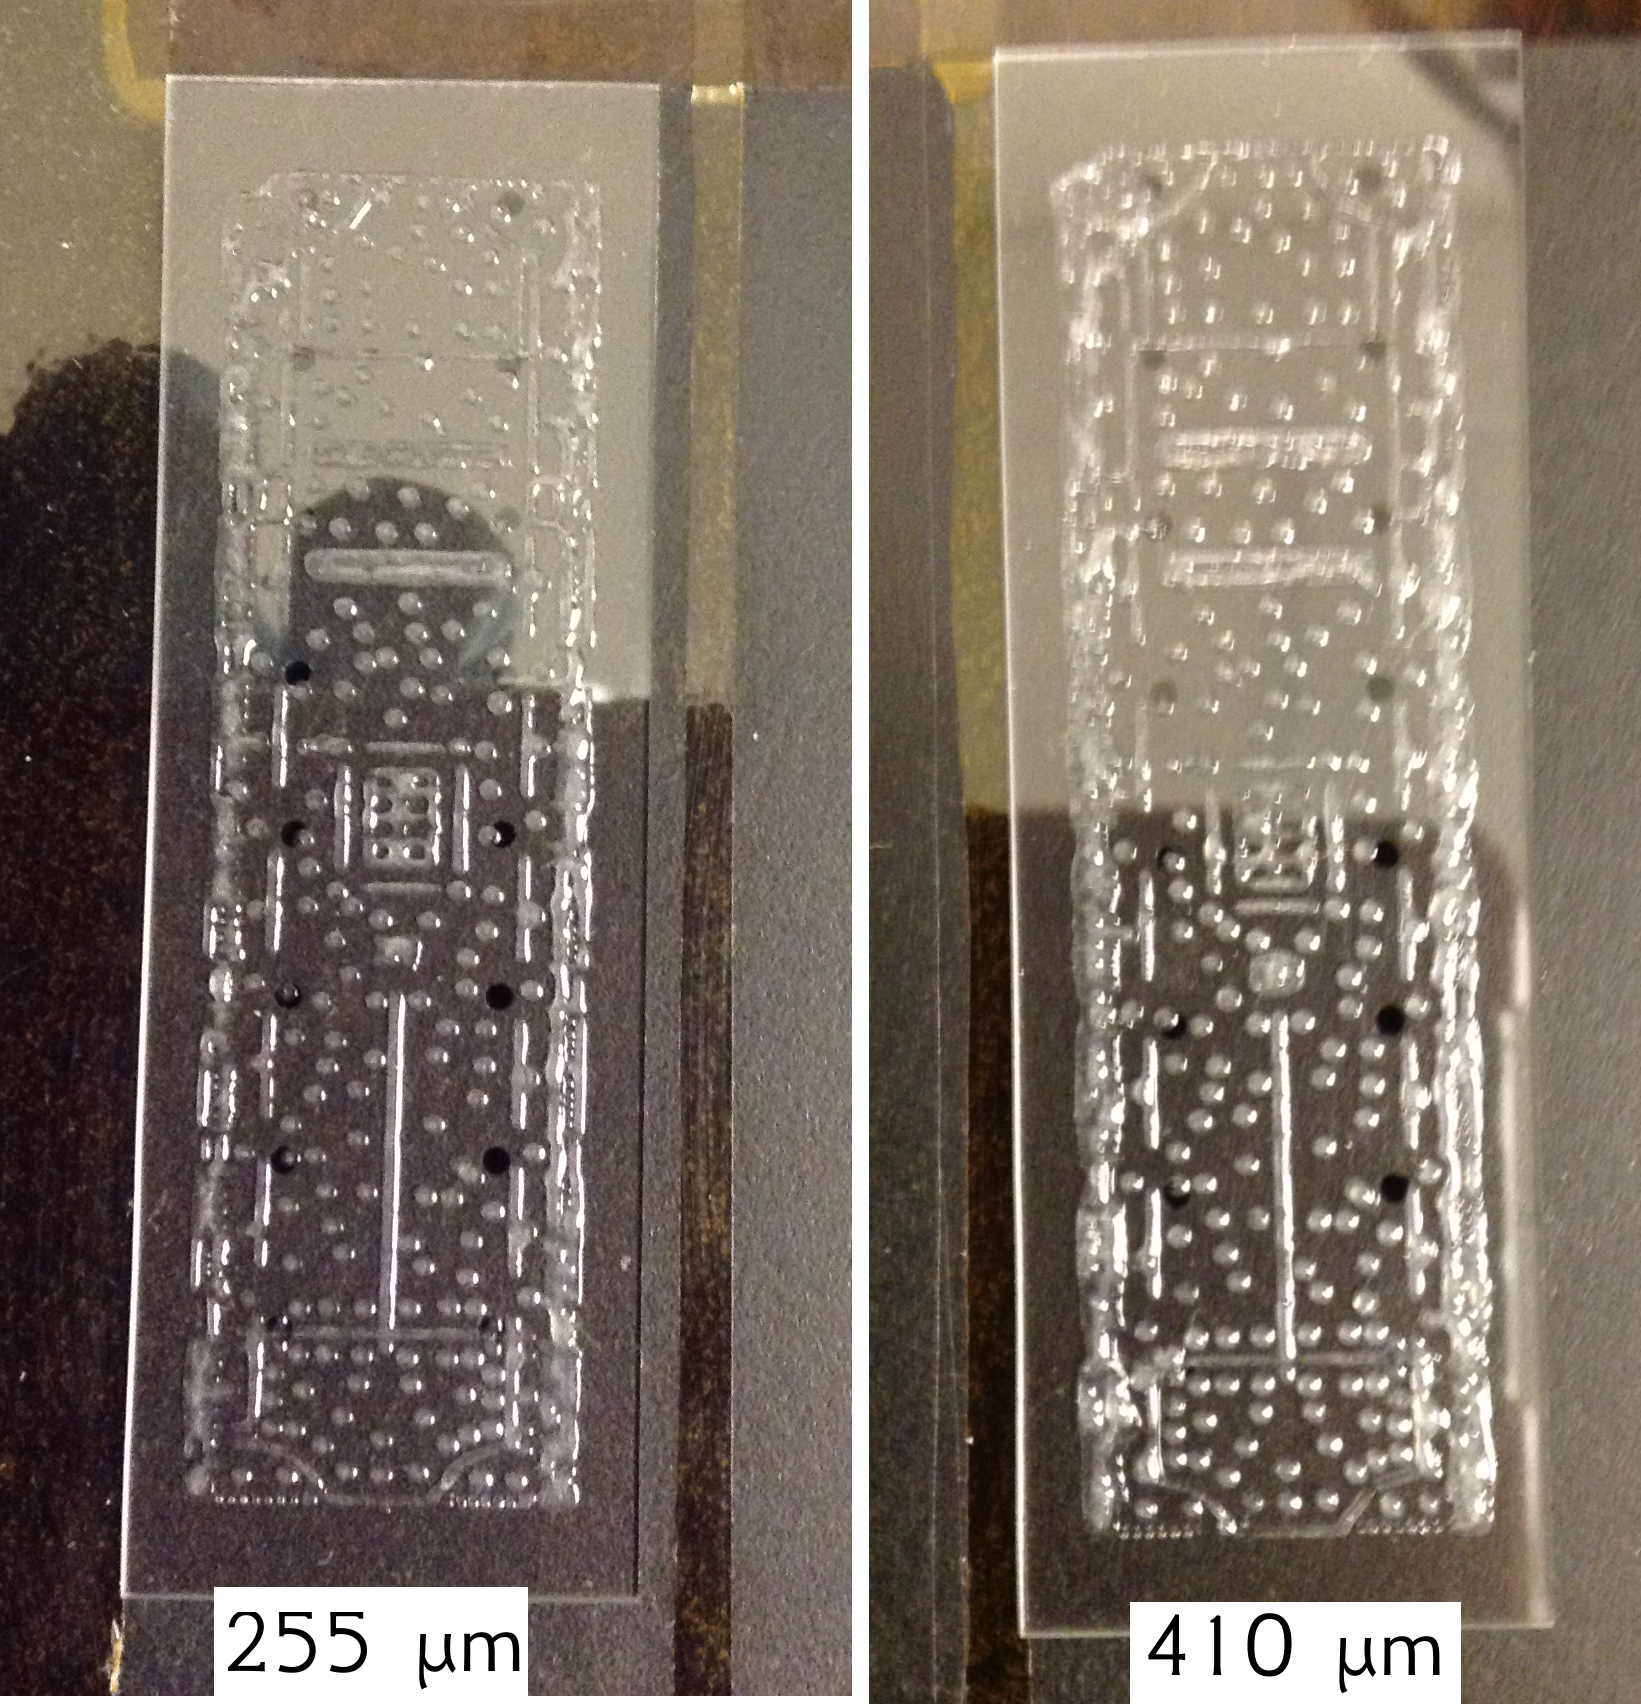
\includegraphics[width=0.4\textwidth, height=0.4\textwidth]{pixel/glue_test_depth2}\\
  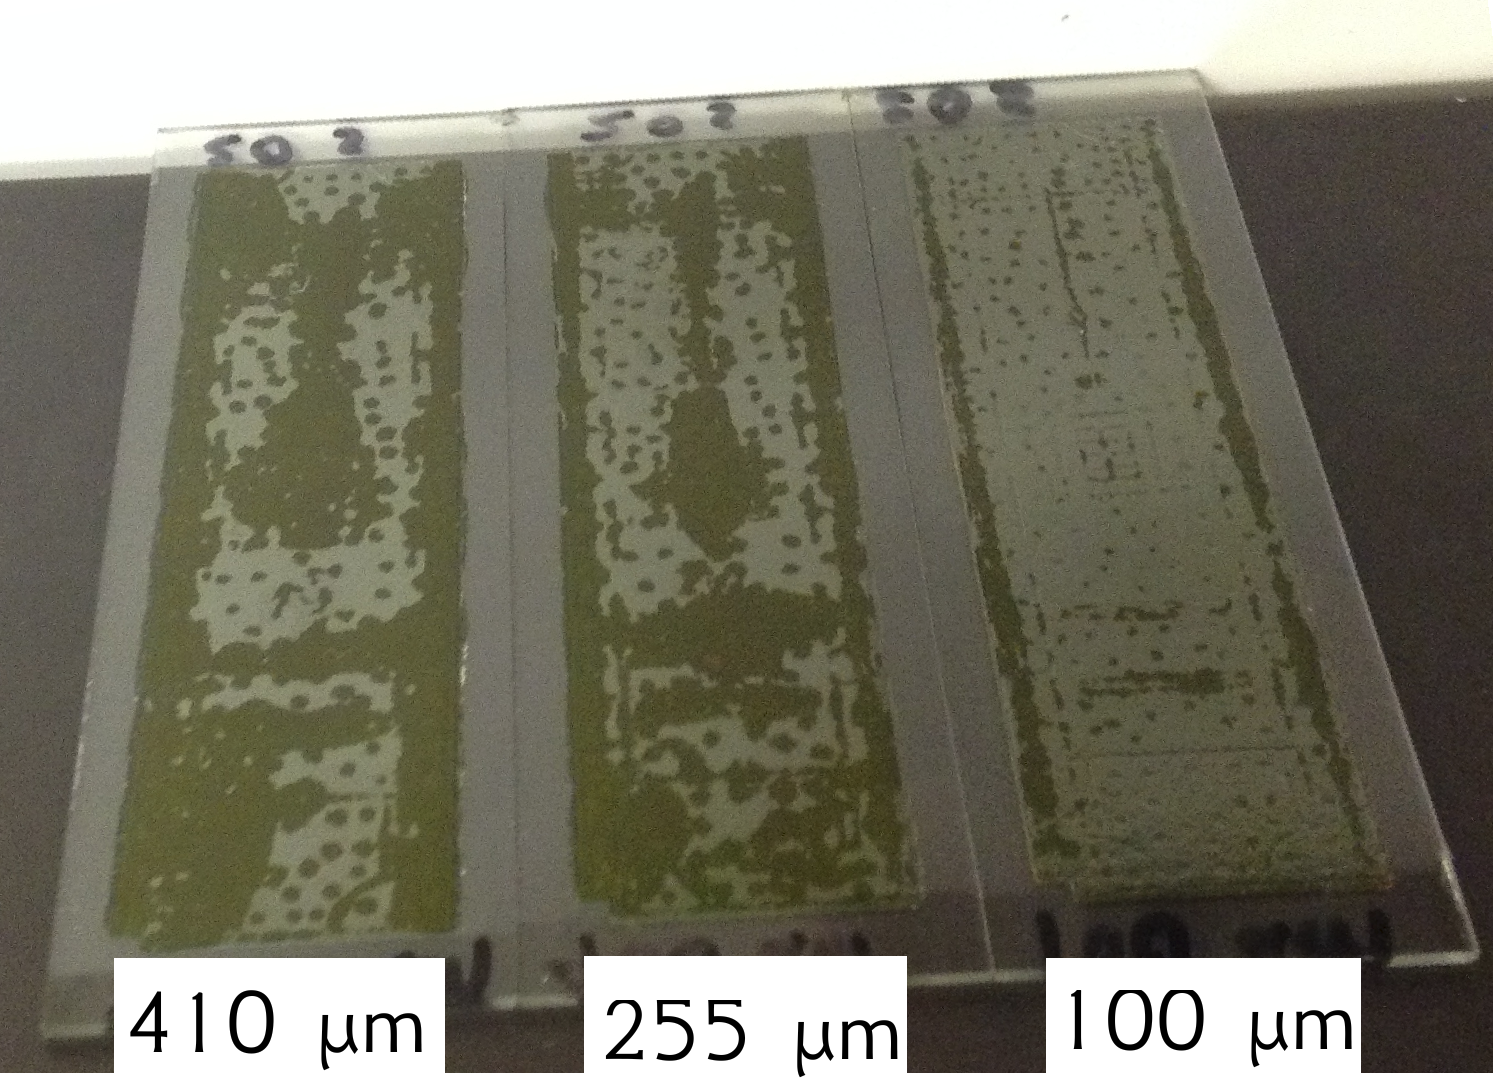
\includegraphics[width=0.6\textwidth]{pixel/glue_test_depth1}
  \caption[Test of amount of glue deposited.]{Pictures of a test of the amount of glue dispensed as a function of the glue reservoir depth. The glue reservoir depth was varied by adding kapton tape (left), and the test were conducted by gluing plain HDI on top of glass slides (middle and right.)}\label{fig:glue_test_depth}
\end{figure}

\item \ti{the amount of glue dispensed}, and in particular the glue spreading out of the HDI area. An excess of glue, scattered beyond the HDI edge would go between the ROC and the sensor, affecting the functionality of the bump bonds connecting them; in the case of the high voltage (HV) pad, it was observed that excess of glue covered the pad on the sensor, making impossible to wire it. The amount of glue deposited on  top of BBM depends on several variables: the dipping time of the stamp tool in the glue reservoir, the time that the stamp tool is in contact with the BBM, and the depth of the glue reservoir. In the case of the dipping and stamping times, it was found that there is not a strong dependence and those times were set to 10 seconds; in the case of the glue reservoir depth, the dependence is stronger. Several glue tests where conducted by gluing plain HDIs to glass slides; Figure~\ref{fig:glue_test_depth} shows pictures from a glue test with three different glue reservoir depths (100 $\mu$m, 255 $\mu$m and 410 $\mu$m). The results show not only that the deeper is the glue reservoir the bigger is the amount of glue deposited, as expected, but also that the spreading out is critical for the depths greater than 200 $\mu$m. A redesign of the rubber stamp pattern was made in order to reduce the amount of glue deposited in the HDI pads regions; that adjustment led to the final rubber stamp pattern.

\begin{figure}[!h]
  \centering  
  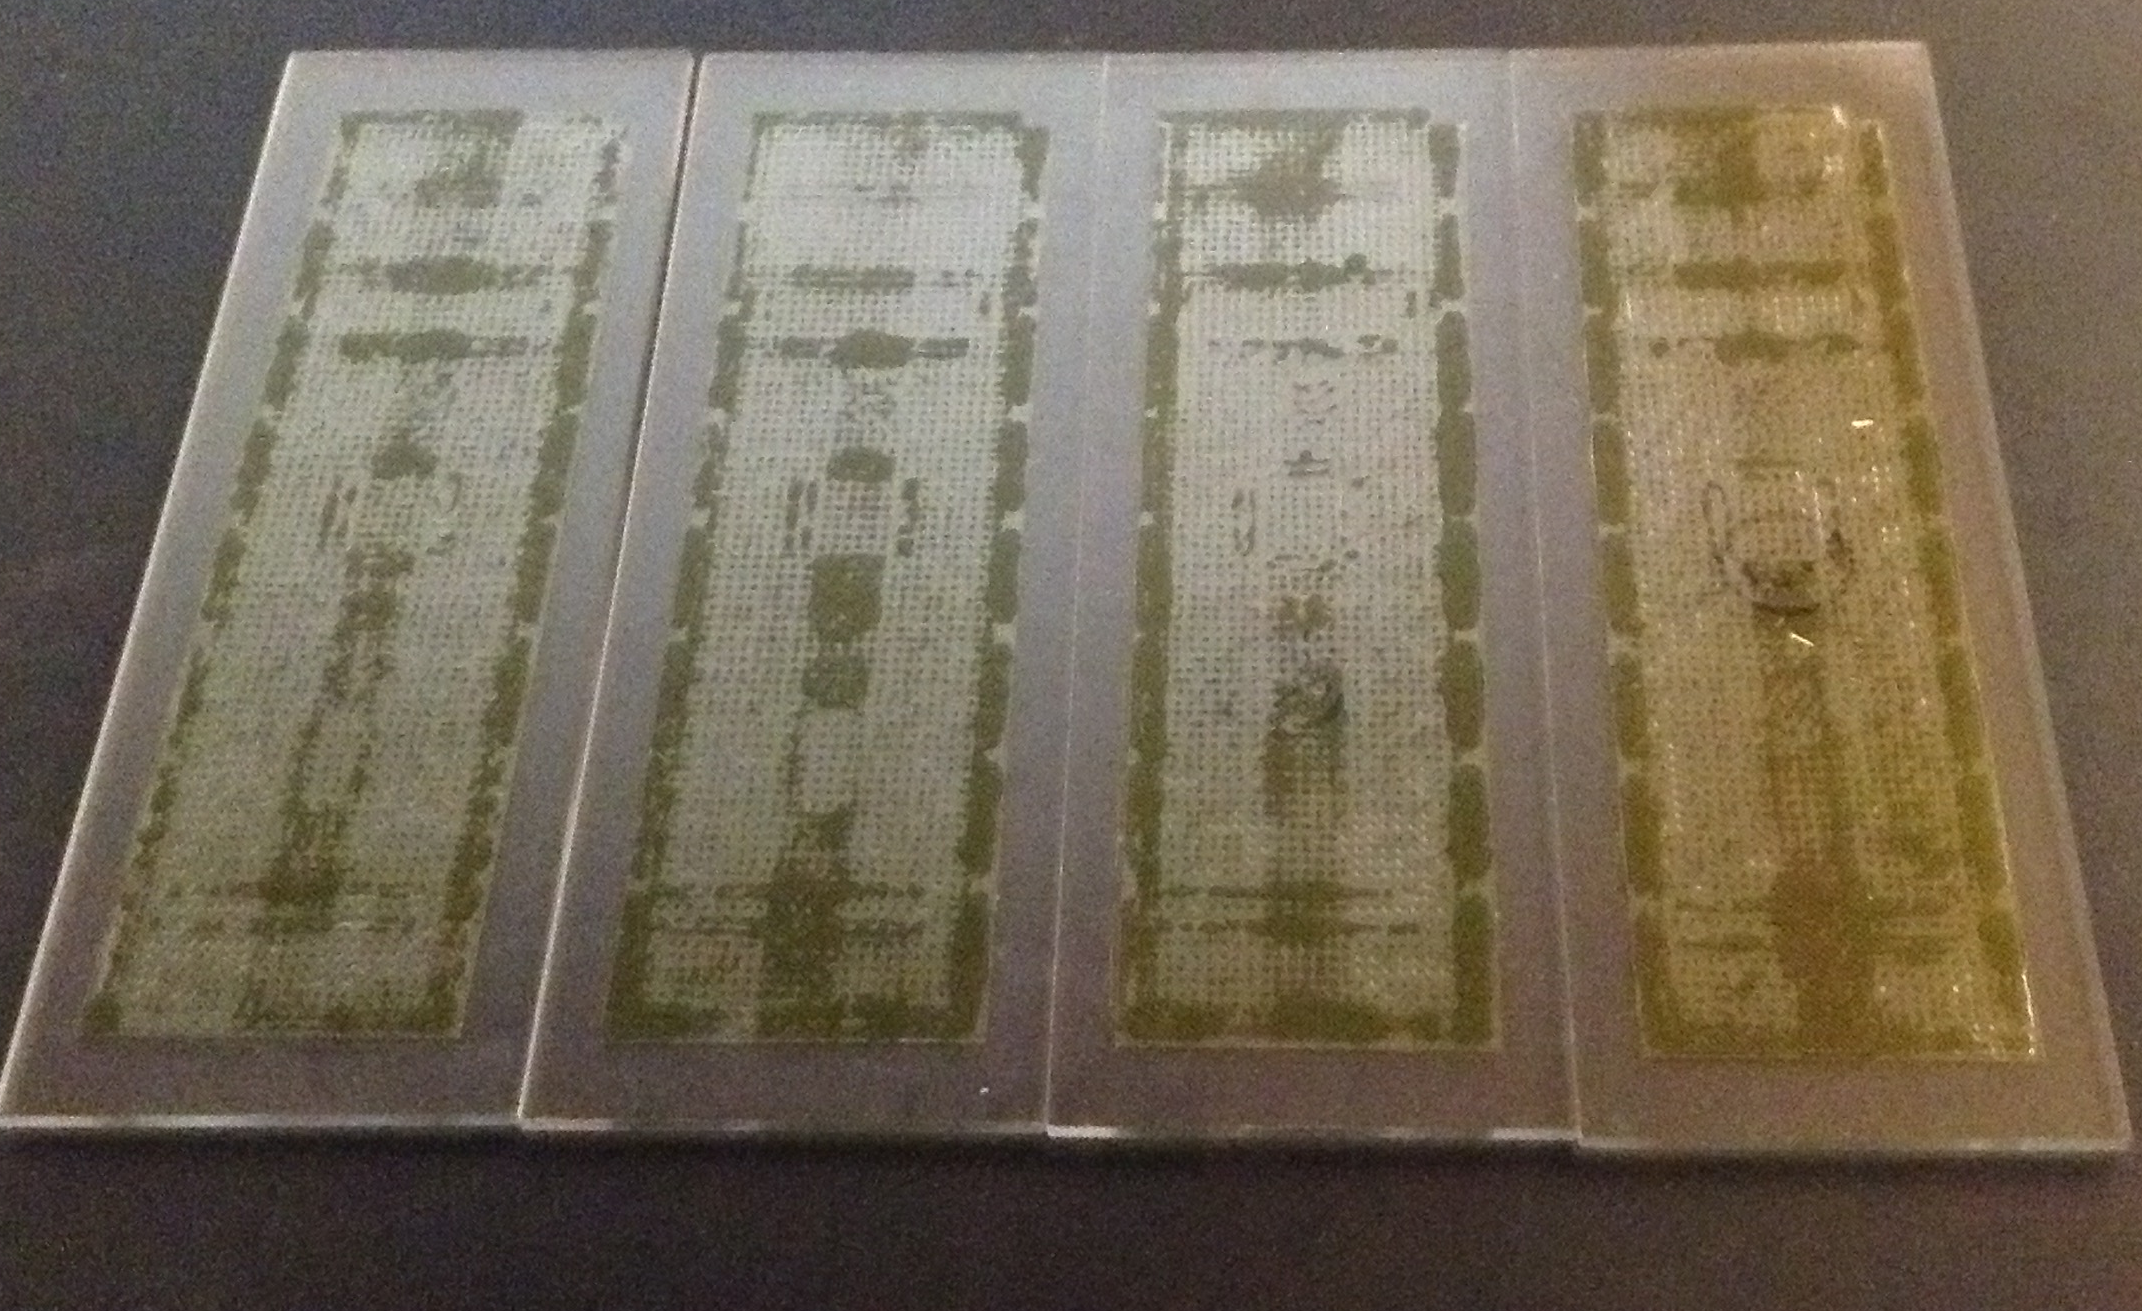
\includegraphics[width=0.6\textwidth]{pixel/glue_test_contact1}\\
  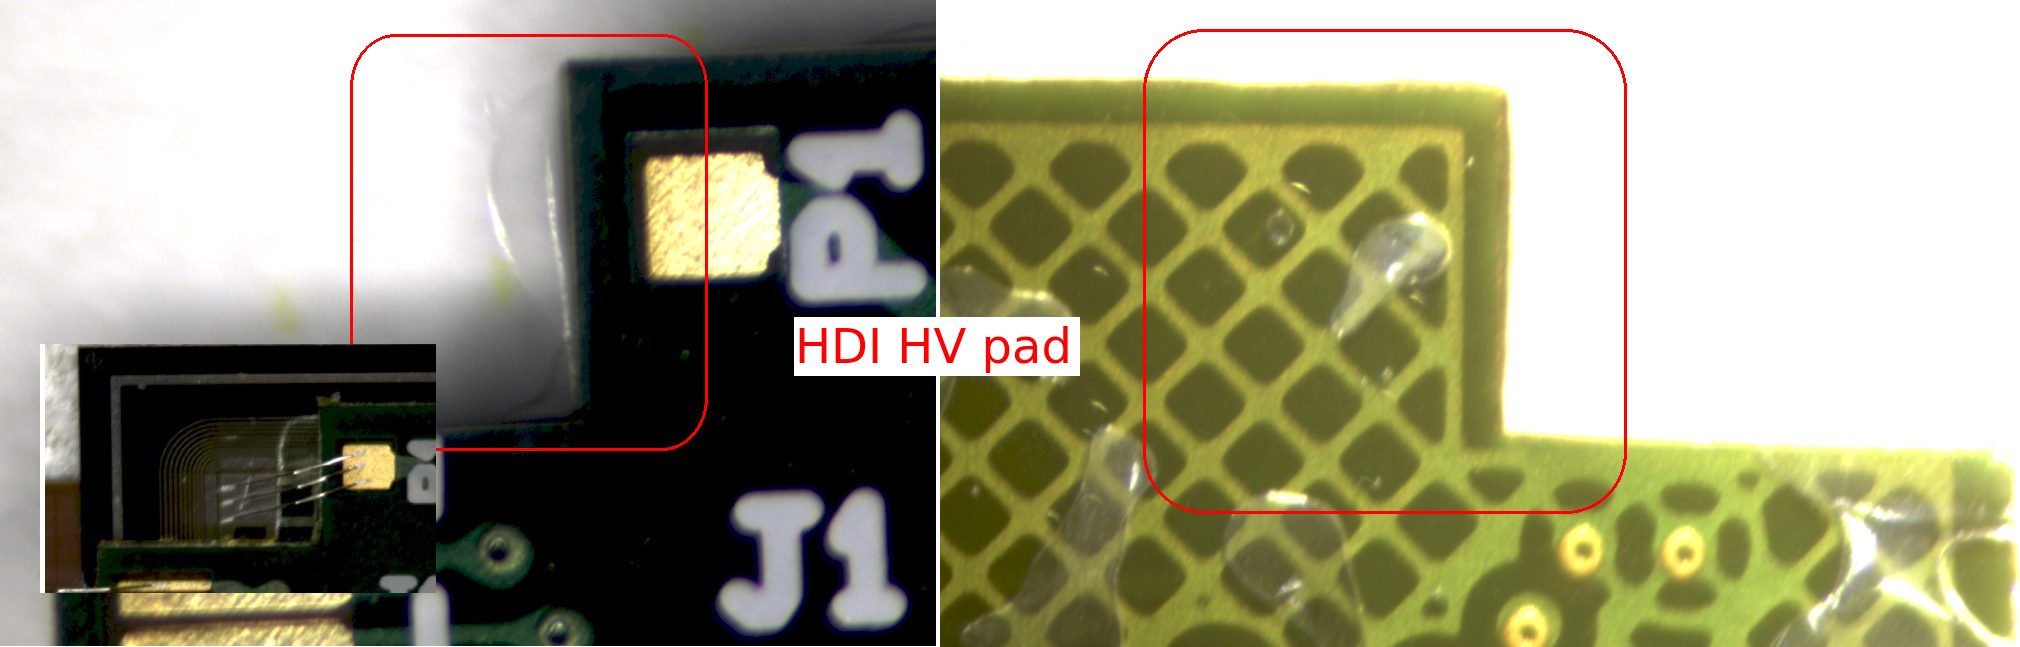
\includegraphics[width=0.8\textwidth]{pixel/hd_pad1}
  \caption[Glue contact area test.]{Results from a glue test using the final stamp pattern, which proves the support provided to the HDI bond pads and the HV pad and the almost null glue spreading out.}\label{fig:glue_test}
\end{figure}

\item \ti{the size of contact area}, and in particular the support given to the edges of the HDI where the bond pads and the HV pad are located. This is a critical aspect, given that the wirebonding relies on the steadiness of the pads to be connected. Figure~\ref{fig:glue_test} shows the outcomes of a glue test using the final stamp pattern. Note the support that it provides to the HDI bond pads and the HV pad and the almost null glue spreading out, which justify why it was chosen.   
\eit

The final tools designs used during the module production are indicated in Figures \ref{fig:st_wt} and \ref{fig:stamp_pattern}, while the optimal glue reservoir depth was found to be 100 $\mu$m. 

\subsubsection*{Grabber and picker tools}

\begin{figure}[!h]
  \centering  
  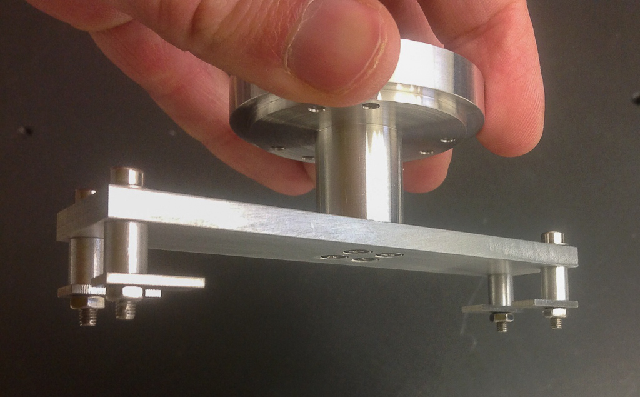
\includegraphics[width=0.60\textwidth,height=0.33\textwidth]{pixel/grabber}\\
  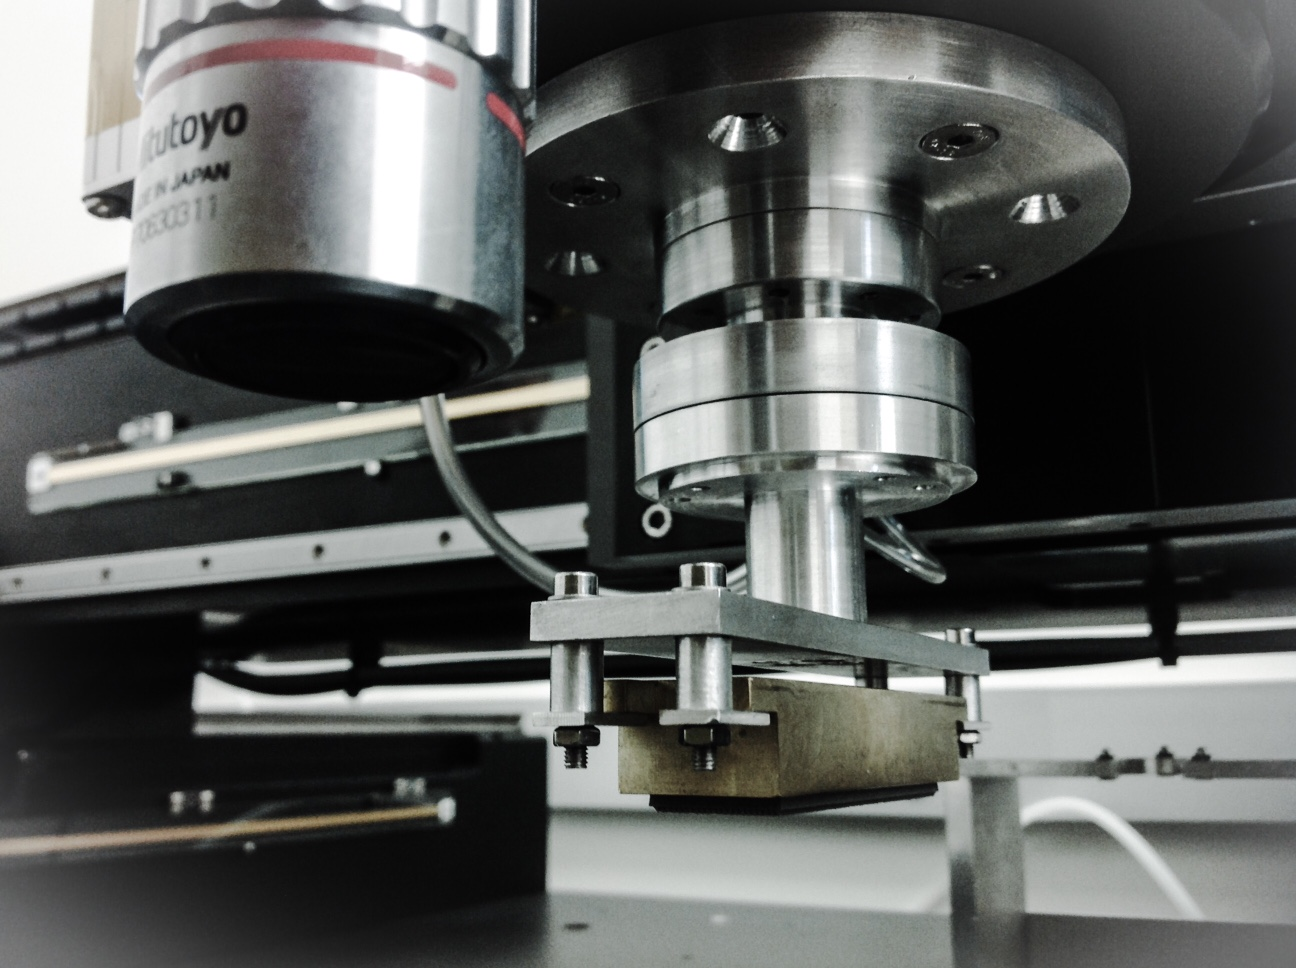
\includegraphics[width=0.45\textwidth,height=0.33\textwidth]{pixel/GrabberToolHoldingStamp}
  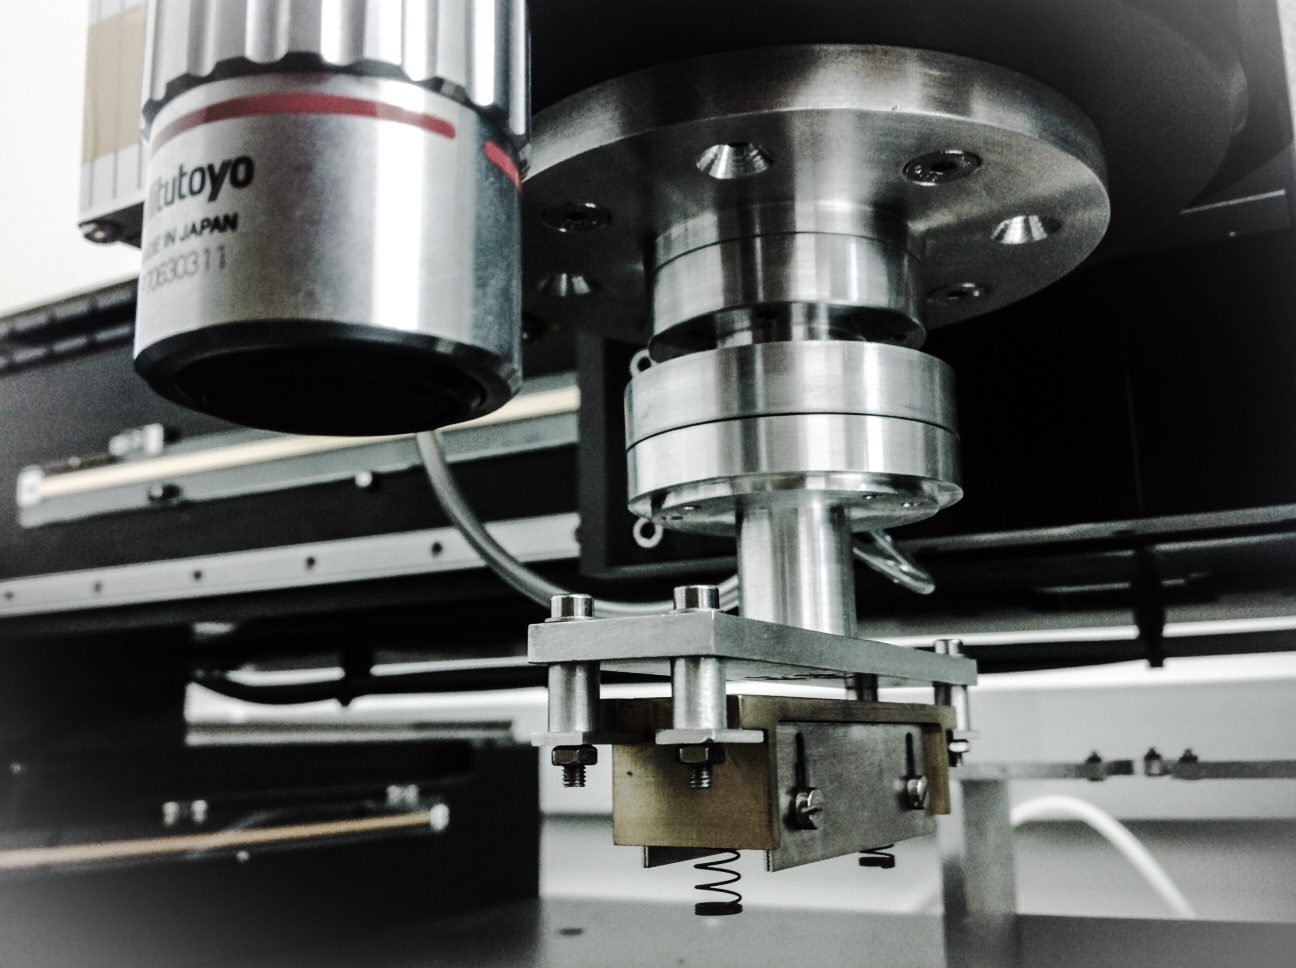
\includegraphics[width=0.45\textwidth,height=0.33\textwidth]{pixel/GrabberToolHoldingWeight}
  \caption[Grabber tool.]{Top: Grabber tool used to grab the stamp and weight tools from their houses to the BBM location. Bottom: grabber tool holding the stamp (left) and weight (right) tools.}\label{fig:grabber_tool}
\end{figure}

In order to move the stamp and weight tools from their houses to the glue reservoir and to the BBM location, a \ti{grabber tool} was designed. The grabber tool is hold on a tool rack located in the back of the gantry table and it gets attached to the gantry head by using an adapter and the vacuum system as shown in Figure\ref{fig:grabber_tool}. The gantry head adapter is attached to the rotary motor that provides the angular motion, therefore, the grabber tool is able grab the stamp and weight tools and adjust their alignment in agreement with the BBM orientation. The force with which the glue is applied on the BBM is controlled by the weight of the brass piece; in a similar way, the force applied to the HDI-BBM sandwich is controlled by the weight of the tool and the springs.                  

The pick of the HDI and place on top of the BBM is performed using the \ti{Picker tool} showed in Figure \ref{fig:pandp_tool}. Same as the grabber tool, the p\&p tool is hold at the tool rack until the gantry head goes to its location and catch it using the vacuum; an independent vacuum line is use to capture the HDI from its chuck slot. The alignment is performed while the HDI is being moved to the BBM location.      
\begin{figure}[!h]
  \centering  
  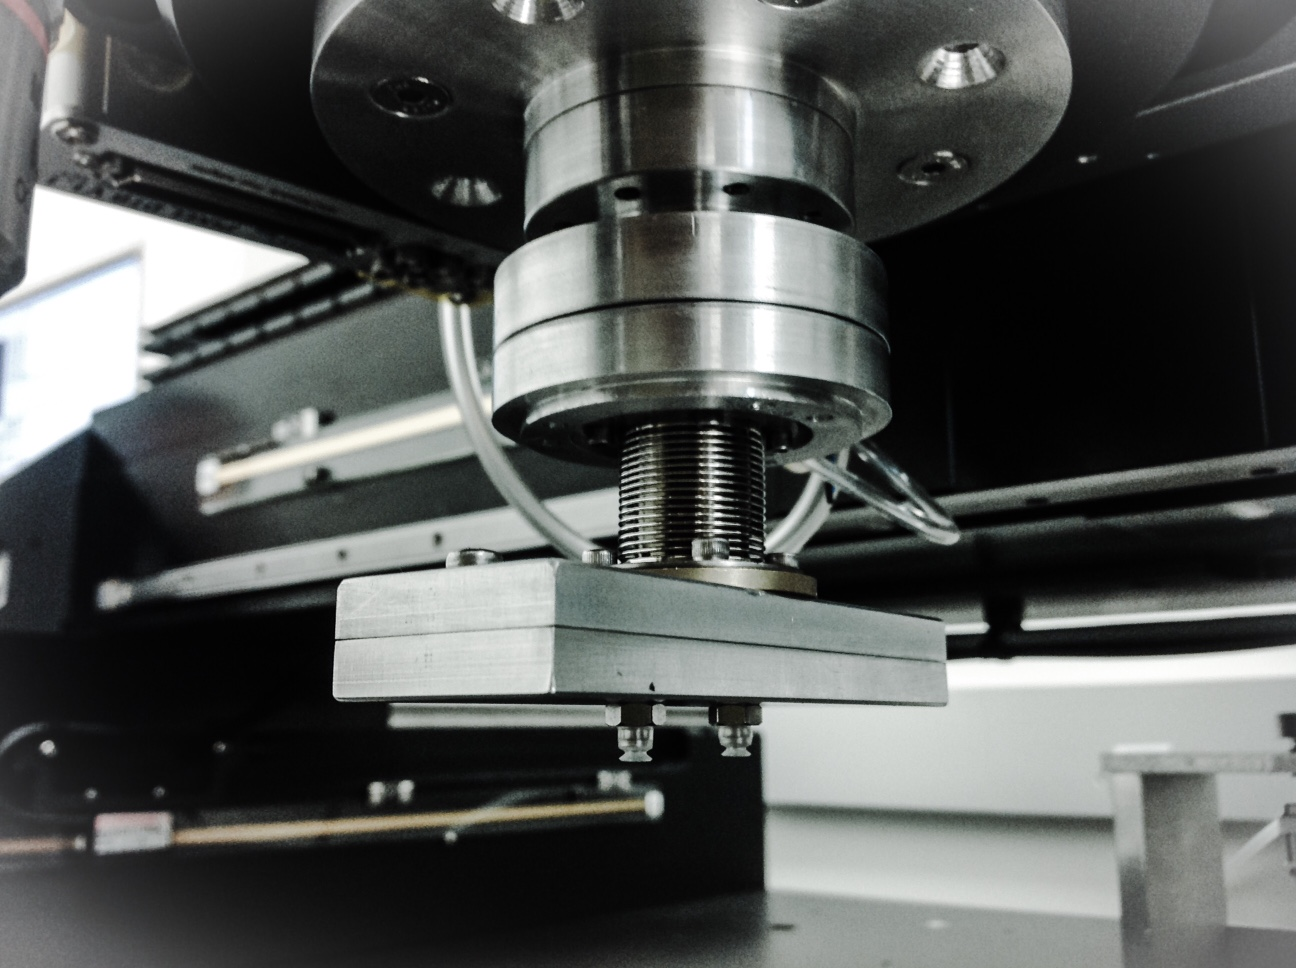
\includegraphics[width=0.80\textwidth]{pixel/PickAndPlaceTool}\\
  \caption[Pick and place tool.]{The pick and place tool, picks the HDI from its chuck and place it on top of the BBM.}\label{fig:pandp_tool}
\end{figure}

\subsubsection*{Vision system}

A vision hardware system, attached to the gantry head, is used to locate the module components and tools employed in the assembly process. It is composed of a IDS HD digital camera and a Mitutoyo wide-field video microscope unit (WIDE VMU) as shown in Figure \ref{fig:setup}. The vision hardware is complemented with auto-focus and pattern recognition algorithms. 

\begin{figure}[!h]
  \centering  
  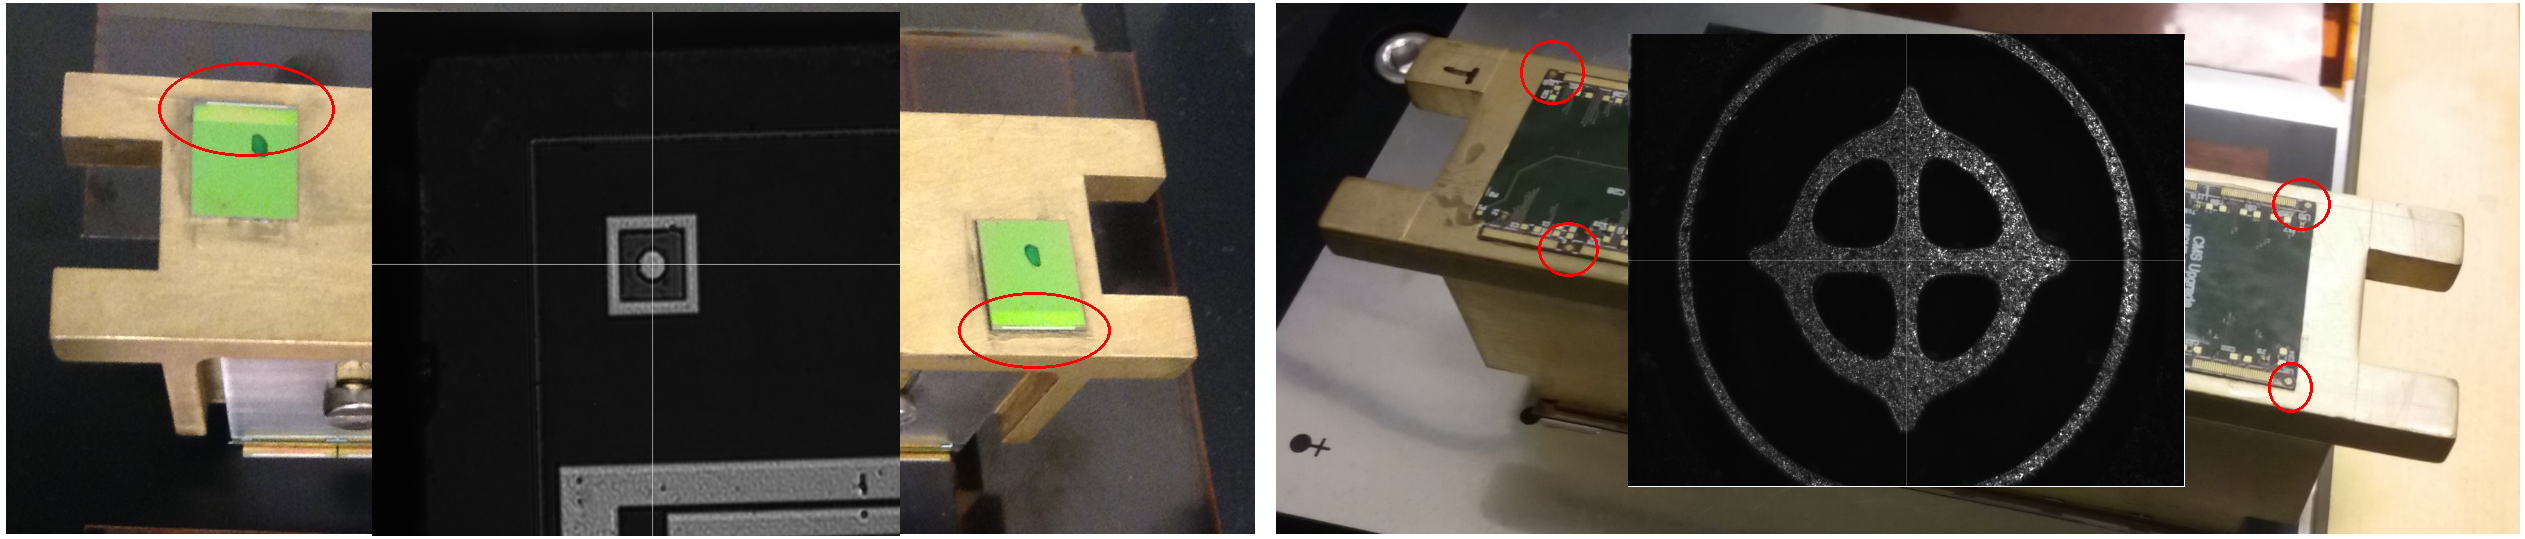
\includegraphics[width=\textwidth]{pixel/fiducial_tools}\\
  \caption[Fiducial marks on tools.]{Fiducial marks attached to the stamp and weight tools. Initially, non-functional ROCs were glued on top of the tools (left) to provide the marks, located in the places indicated by red circles and showed overlaping the tool; later they were replaced by plane HDIs (right).}\label{fig:fiducial_tools}
\end{figure}

Given that the coarse location of the HDIs, BBMs, stamp and weight tools are well defined by the location of the stencils and plates on the gantry table, the vision system is designed to search and find fiducial marks present on the materials and tools; these fiducial marks are placed on the HDI and BBM during their fabrication process. In the case of the tools, two methods were used to attach a fiducial mark to them: non-functional ROCs, which have on themselves fiducial marks, were glued on top of the tools as shown in Figure \ref{fig:fiducial_tools}, however, during the gluing and cleaning processes the fiducial marks used to be covered or broken making necessary their replacement very often; the second method consisted of gluing plane HDIs on top of the tools, which not only solved the issues with the destruction of the fiducial marks but also simplified the pattern recognition.

The procedure to find the fiducial marks starts by moving the camera to an initial default calibrated position above the element, HDI, BBM or tool, such that the image in the field of view of the camera contains the fiducial mark; then, the auto-focus algorithm finds the best focus by measuring the contrast of pictures taken by the camera at ten different positions in $z$ direction around a default position where it is assumed the best focus is; these ten contrasts are then fitted to a Gaussian distribution where the maximum of the fitting corresponds to the best focus.     

Once the best focus is found, the gantry head moves the camera to that position, takes a new picture and send it to feed the pattern recognition algorithm which use k-means clustering to separate the foreground from the background; then, the foreground (Fiducial + noise) is dilated to close any small holes in image and to extract contours from image.

\begin{figure}[!ht]
  \centering  
  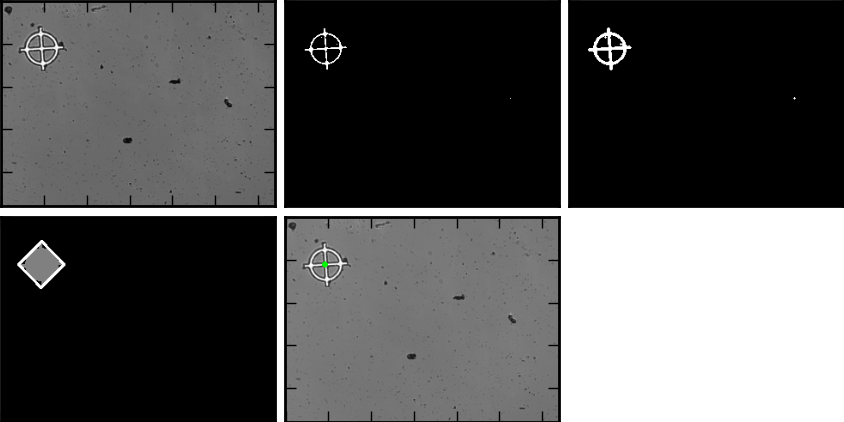
\includegraphics[width=0.8\textwidth]{pixel/BBM_fid1.png}
  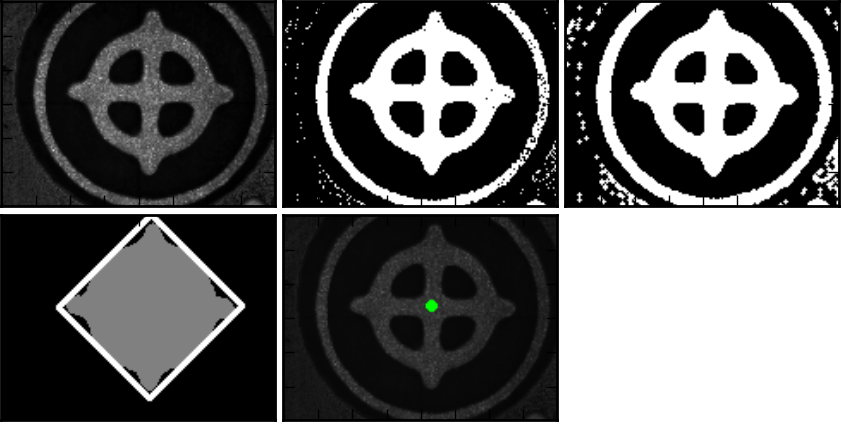
\includegraphics[width=0.8\textwidth]{pixel/HDI_fid1.png}
  \caption[Fiducial mark recognition.]{Fiducial mark recognition: BBM (two top rows) and HDI (two bottom rows). The input image is processed to define contours; after filtering, the centroid of the recognized fiducial mark is returned by the algorithm and indicated in the input image by the green dot.}\label{fig:BBM_fid1}
\end{figure}

The fiducial mark features are parametrized in terms of its size and aspect ratio with respect to the field of view of the camera, therefore, by filtering the contours on size and aspect ratio it is assured that one and only one contour passes filters. Later, the algorithm calculates the minimum bounding box and centroid of the fiducial mark to finally return the centroid as fiducial mark center and distance between centroid and box center as a measure of goodness. In order to reduce the processing time, the input image resolution is reduced by a factor of 8. The algorithm was written by Caleb Fangmeier and is documented in Reference \cite{pr_algorithm} from where Figure \ref{fig:BBM_fid1} was taken.

\subsubsection*{Gantry head center-camera offset (GHCO)}

The \ti{global coordinate system} of the setup is centered in the so-called \ti{home position} located in the back-left side of the gantry table; thus, the origin of the coordinate system is defined by the position of the gantry head center when it is placed in the home position. Any distance is then measured by comparing the gantry head center position at a given location and the home position. While the tool adapter is concentric to the gantry head (and then its coordinates are the same as the gantry), the camera has an offset with respect to the origin of the global coordinate system because the vision system is not located at the gantry head center, therefore, any location provided by the vision system has to be corrected by this offset, known as \ti{Gantry head center-camera offset} (GHCO).

\begin{figure}[h]
\begin{center}
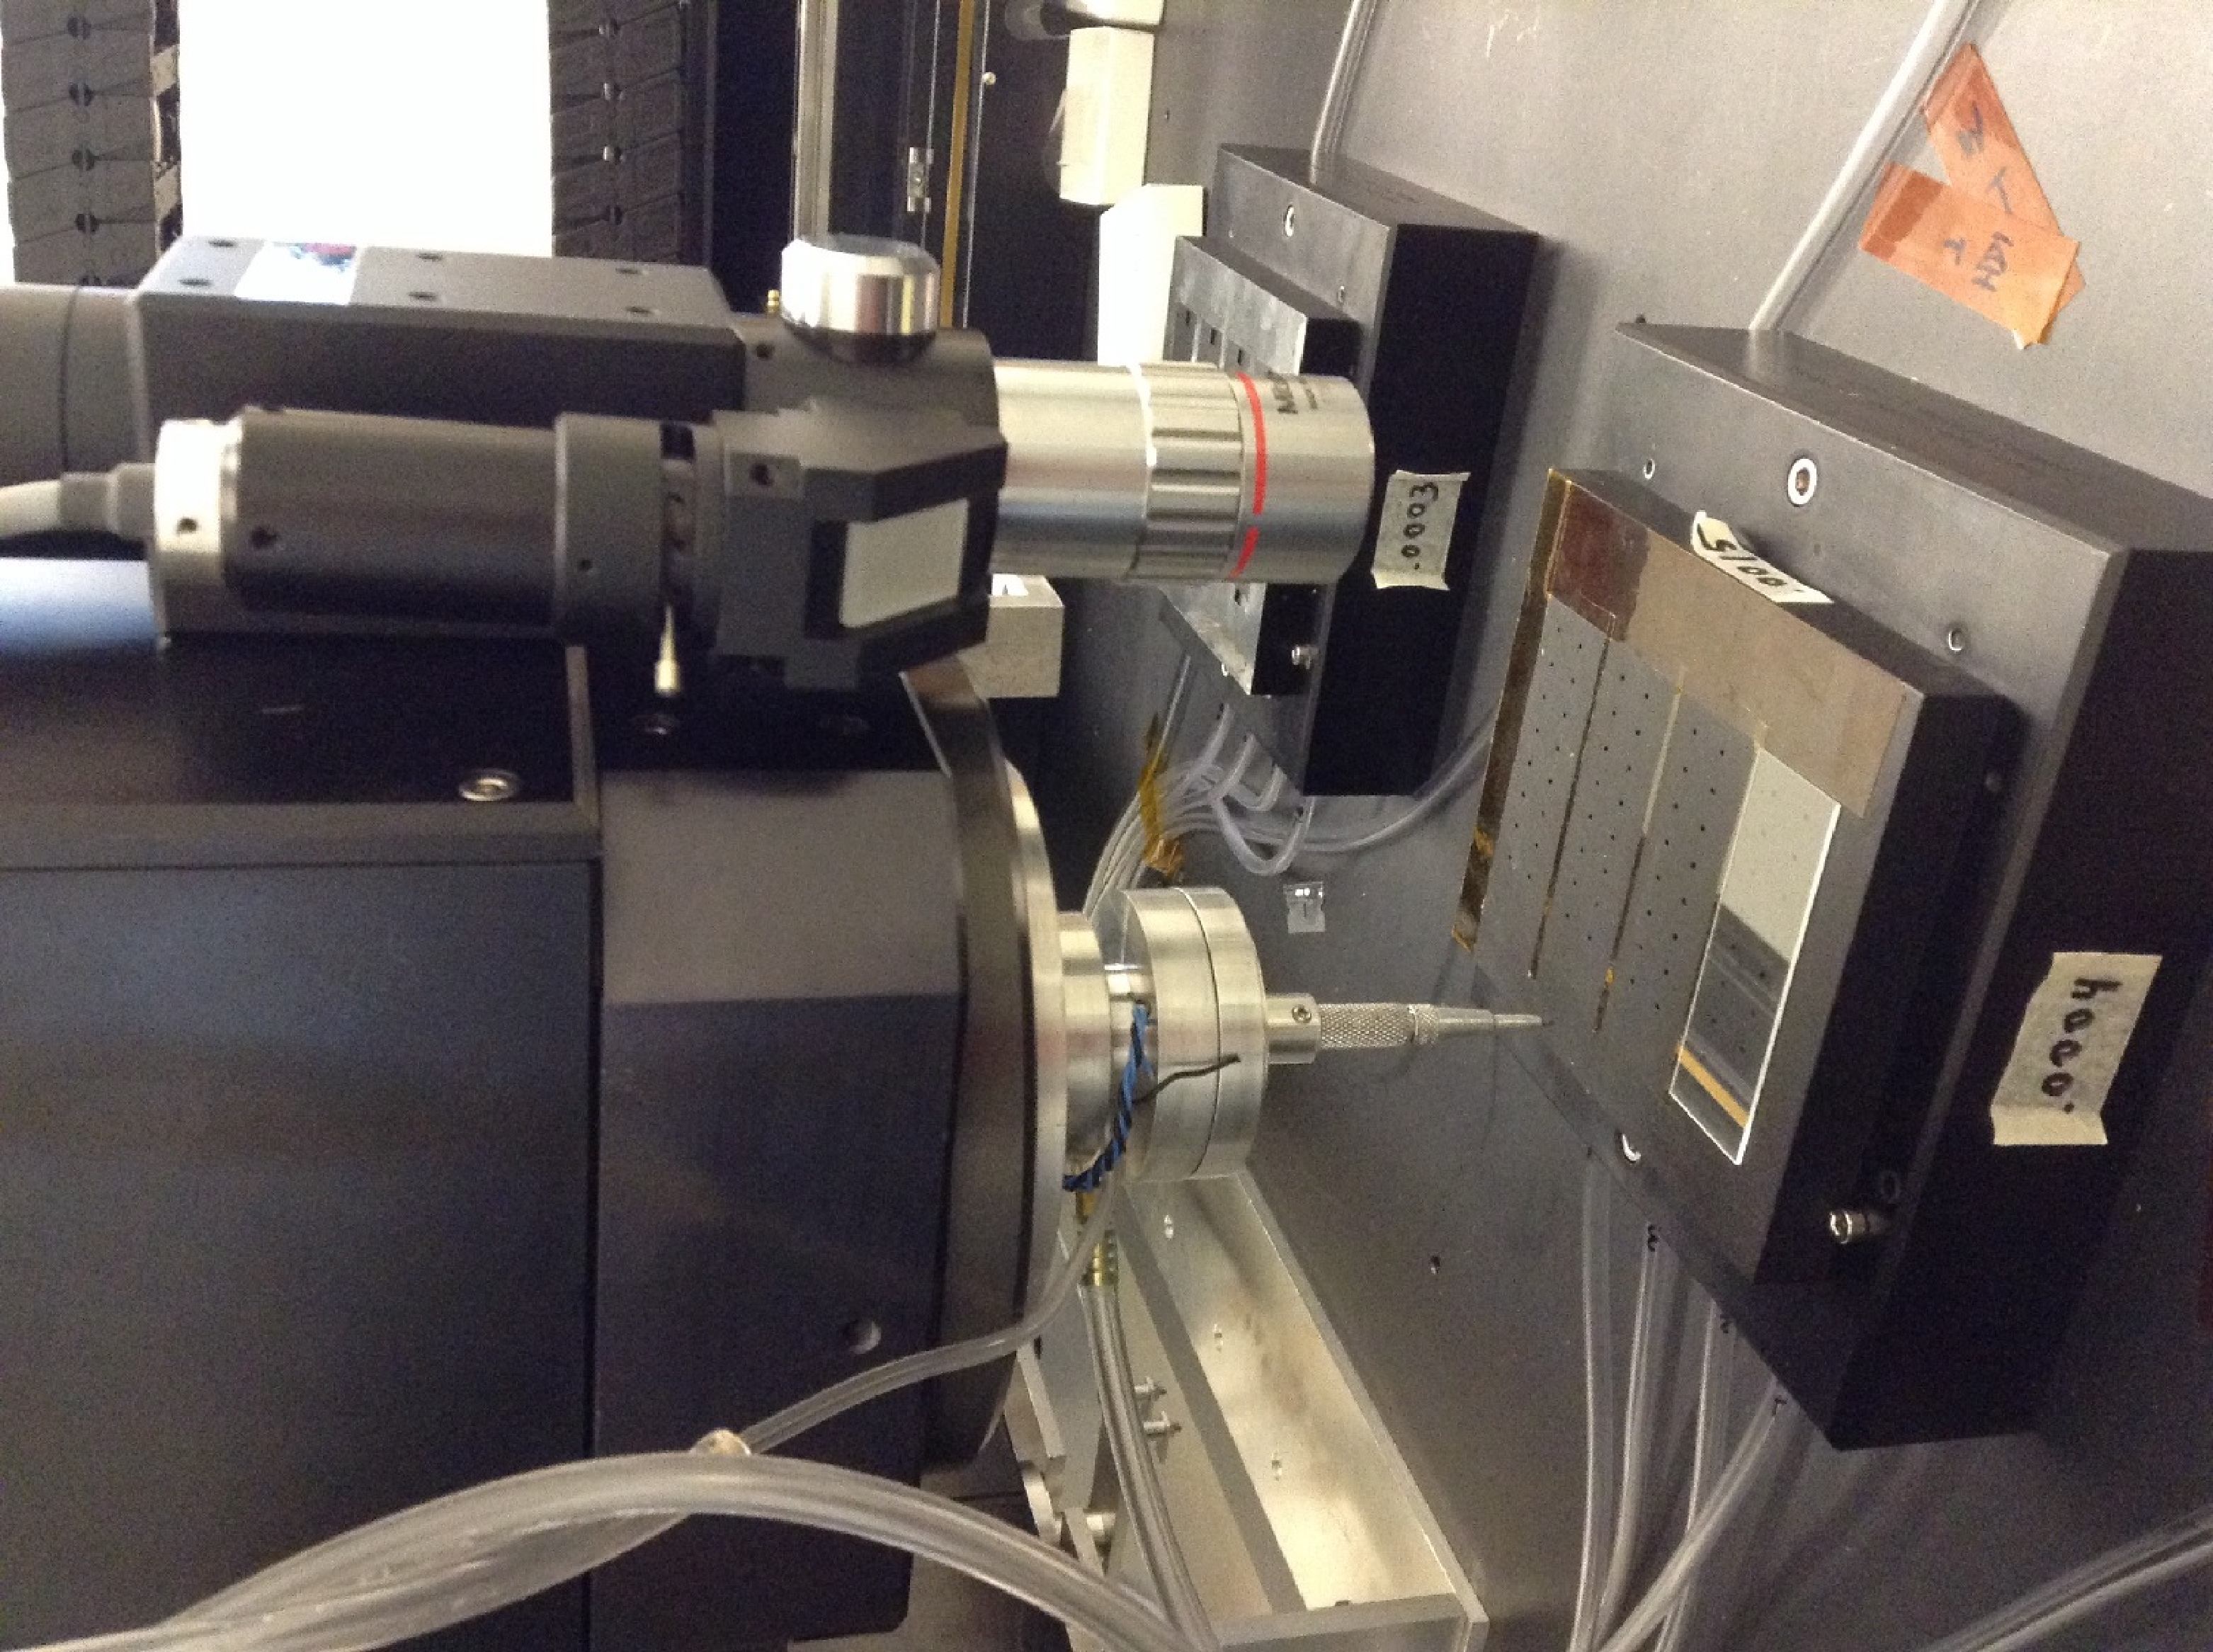
\includegraphics[width=0.45\textwidth,angle=-90]{pixel/offset_setup}
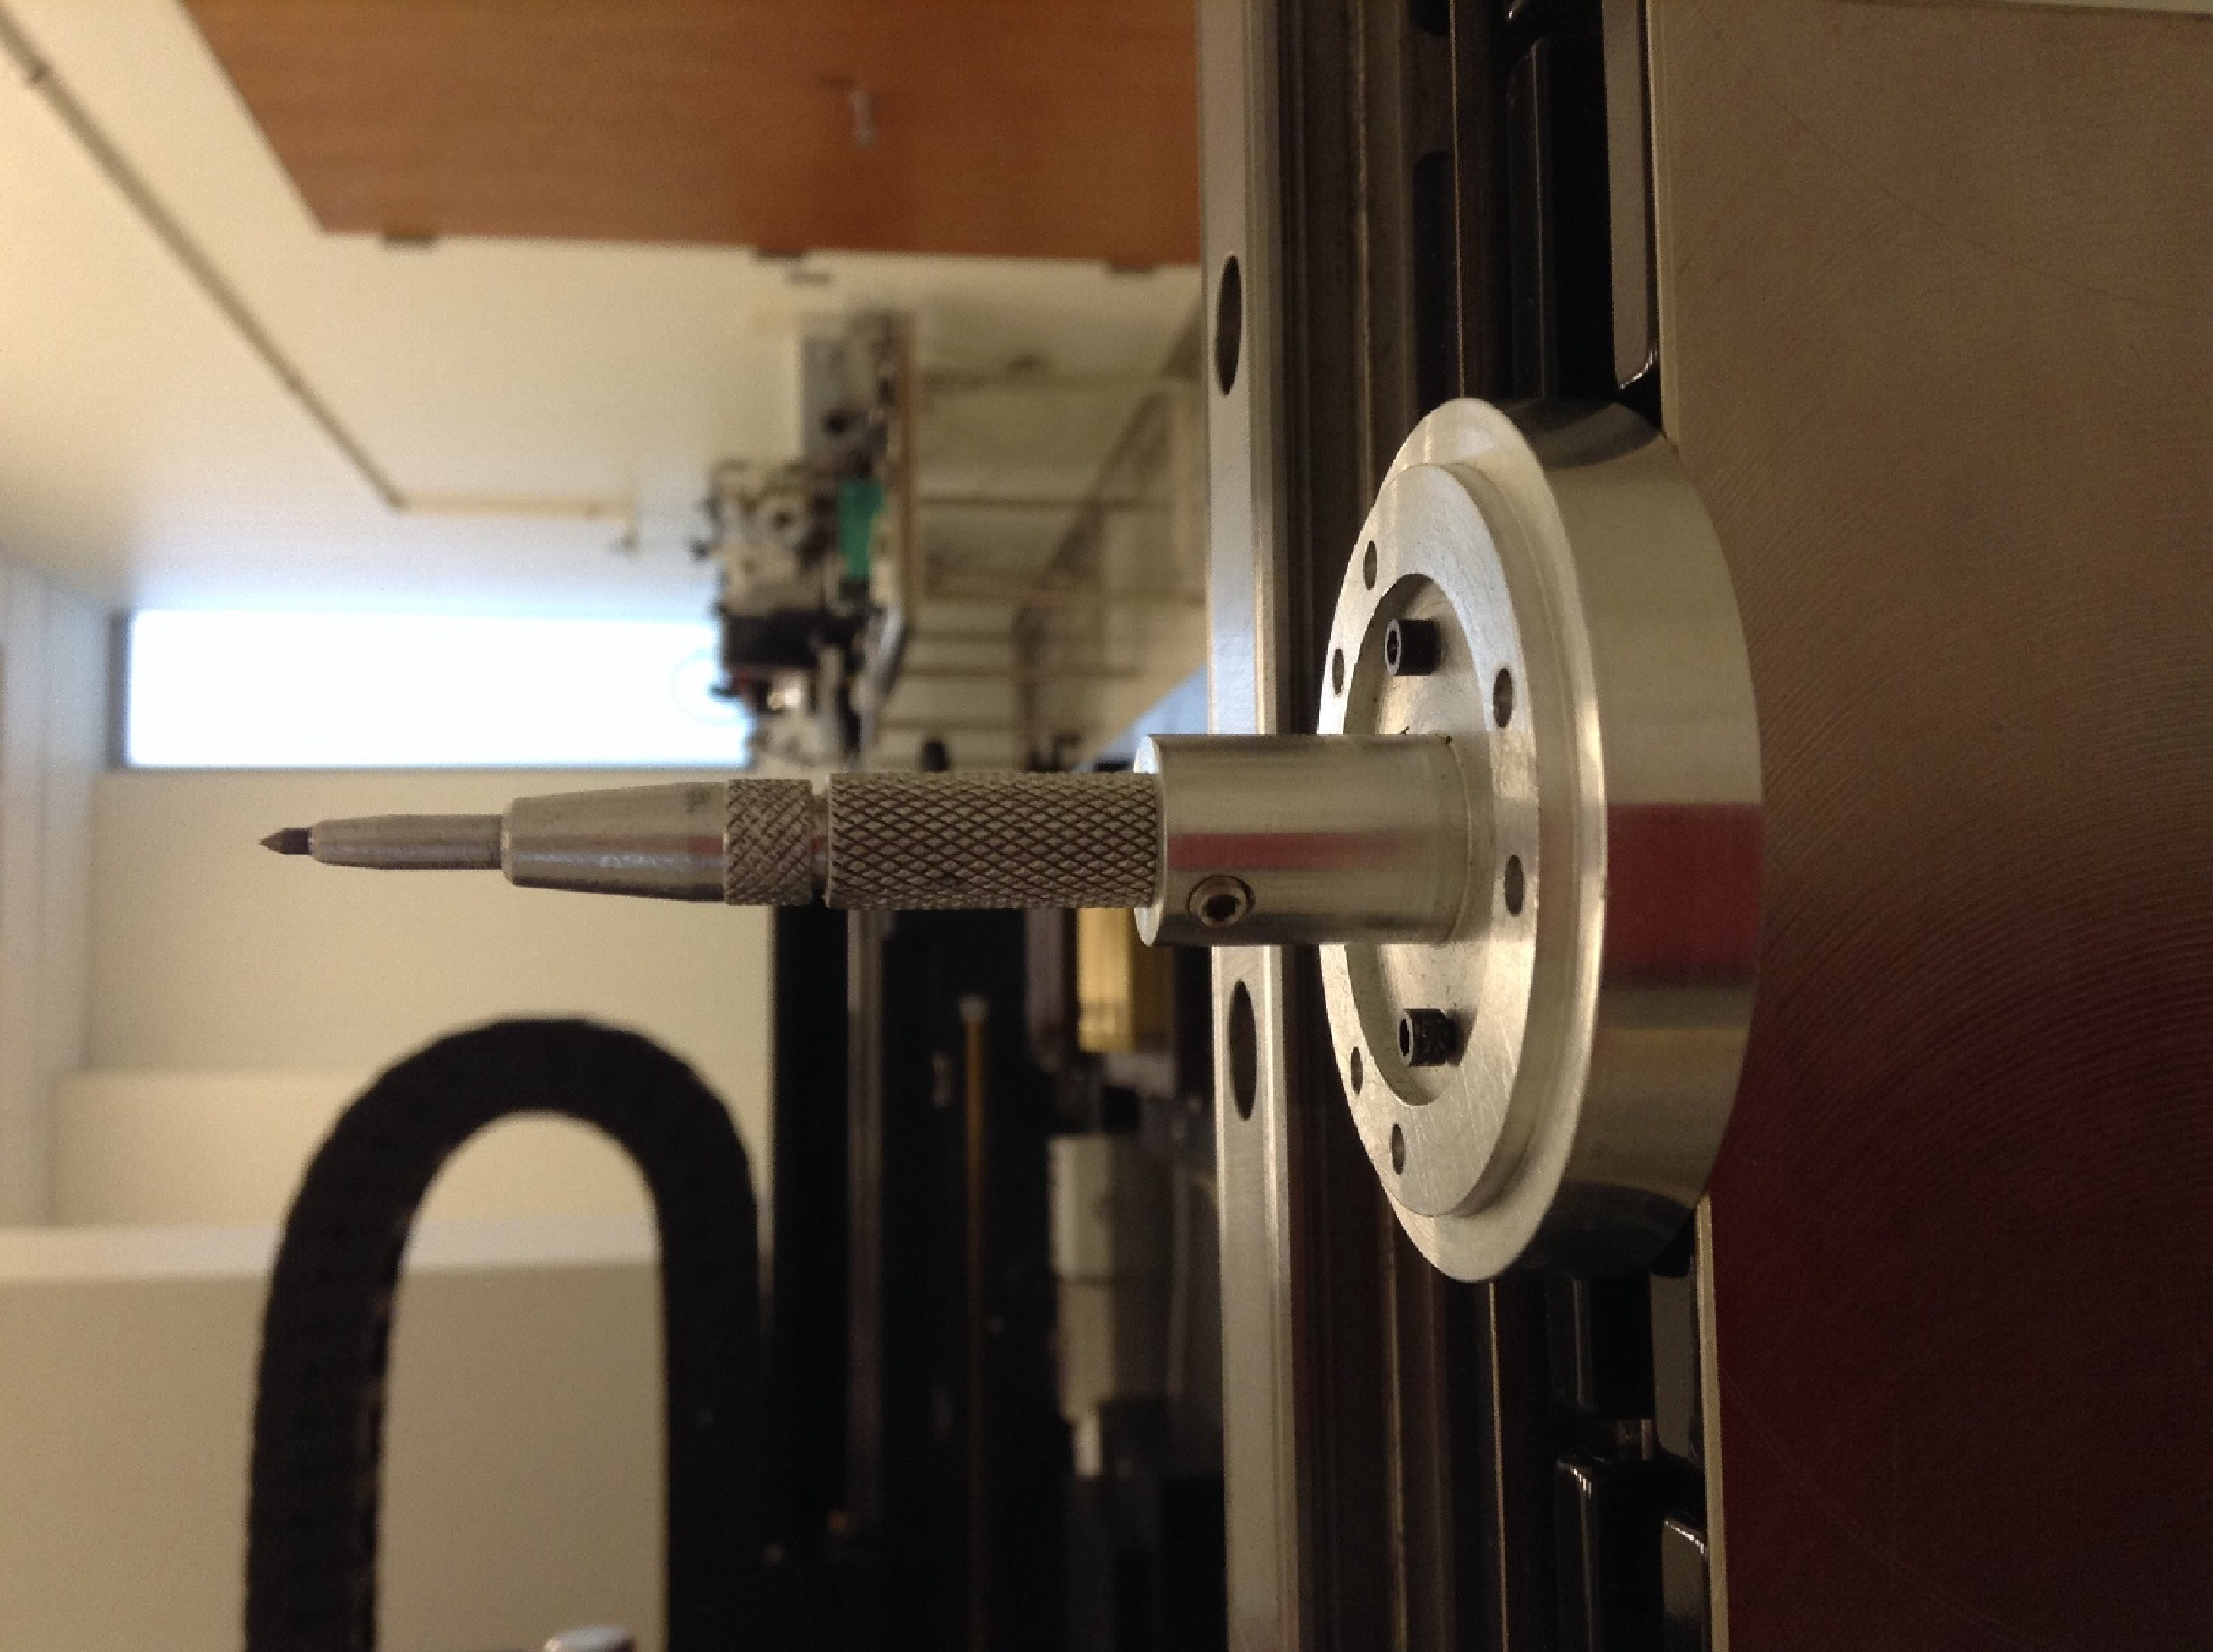
\includegraphics[width=0.45\textwidth,angle=-90]{pixel/scratch_tool}
\caption{Setup used to measure the GHCO}\label{fig:offset_setup}
\end{center}
\end{figure}

To determine the GHCO, a set of 40 marks (scratches) were made on a glass slide using a needle shaped tool with the tip made of carbide (see Figure \ref{fig:offset_setup}); the locations of the scratches were predefined and known as commanded positions. Later, the camera was moved to find the scratches and their locations were tagged as observed positions. In principle, the difference between the commanded and the observed positions provide a measurement of the GHCO, but it cannot be assumed that the needle tool is straight, i.e., if the tip of the tool coincides with the gantry head center; in order to take into account this fact when calculating the offset, an scratching schema was designed; it is showed in Figure \ref{tool_bend}. In the ideal case the scratch is made right in the commanded position (red circle), but if the needle is not straight, the scratch will be shifted (black cross). A rotation of the tool can be used to determine how bend is the needle tip.

\begin{figure}[h]
\begin{center}
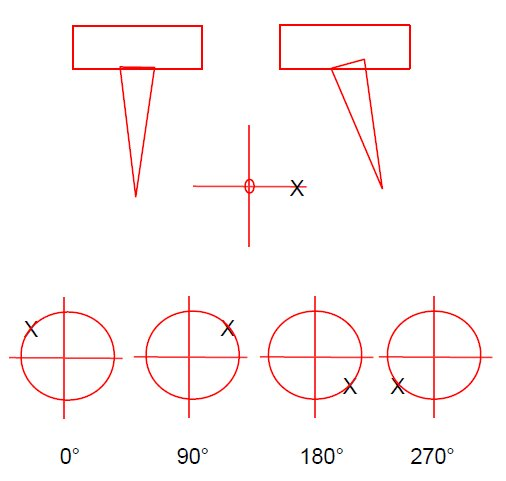
\includegraphics[width=0.7\textwidth]{pixel/tool_bend}
\caption{Scratches scheme if the tool is not straight }\label{tool_bend}
\end{center}
\end{figure}

The precise procedure is:

\begin{itemize}
\item pick the needle tool from the tool rack,
\item move the gantry to the first scratch position (the commanded position),
\item make the scratch moving the tool down.
\item move the tool back up
\item move the gantry to the next scratch commanded position.
\item Repeat the process to make nine more scratches.
\item Rotate the tool by $\theta=90^o$ and make ten scratches.
\item Rotate the tool by additional $90^o$ (now the total rotation is $\theta=180^o$) and make ten more scratches.
\item Rotate the tool by additional $90^o$ (now the total rotation is $\theta=270^o$) and make ten more scratches.
\item Move the camera to the first scratch position and locate the center of the scratch, capture the position.
\item Repeat the process to locate the rest of the scratches.   
\end{itemize}

The procedure is performed by a labVIEW program (\ti{offset\_fitting.vi}) which follows the steps mentioned above automatically so that the user only interacts with the program by capturing the positions. The output of the program is a text file which contains all the commanded and observed positions.
      
The set of measurements are statistically treated, using the linear least squares fitting technique. The model describing the location of the scratches system is parametrized by a linear combination of a set of functions weighted by a set of parameters;

\begin{equation}
y(x)= f(y,\textbf{a})=a_1f_1(x)+a_2f_2(x)+.....+a_pf_p(x)
\end{equation}

The residuals, which correspond to the difference between the predicted value from model ($f(x_i, \textbf{a})$) and the measured value $y_i$, are calculated using 

\begin{equation}
r_i= y_i - f(x_i\textbf{a}),
\end{equation}

\noindent one want to minimize these residuals and more specifically their squares (S). The fit will provide the values of the parameters $\textbf{a}$ so that the model is totally defined. In matrix form, for a set of measurements $(x,y)$ :

\begin{equation}
\textbf{Y}= A \textbf{a}
\end{equation}
\begin{equation}
S=\textbf{r}^T\textbf{r}
\end{equation}

The matrix A enclose the features of the system/model, the vector \textbf{a} enclose the parameters under evaluation and the vector \textbf{Y} enclose the measurements taken and the predictions made by the model. After the minimization, the vector of parameters can be written as:

\begin{equation}\label{solution}
\textbf{a}=(A^TV^{-1}A)^{-1}A^TV^{-1}\textbf{Y}
\end{equation}

\noindent where V is the covariance matrix; it contains the information about the correlation among measurements and also the uncertainty of the measurements.

\begin{equation}
  V=
  \begin{pmatrix}
    \sigma_1^2  & \sigma_{12}  & \cdots & \sigma_{1n} \\
    \sigma_{21} & \sigma_2^2   & \cdots & \sigma_{2n} \\
    \vdots      & \vdots       & \ddots & \vdots      \\
    \sigma_{n1} & \sigma_{n2}  & \cdots & \sigma_n^2
  \end{pmatrix}
\end{equation}

The model for one measurement $(x,y)$, \ie only one scratch, can be written as:

\begin{equation}
\begin{pmatrix}
x\\ 
y
\end{pmatrix}-
\begin{pmatrix}
x_g\\ 
y_g
\end{pmatrix}=
\begin{pmatrix}
\Delta x_{GHCO}\\ 
\Delta y_{GHCO}
\end{pmatrix}
+
\begin{pmatrix}
c  & s\\ 
-s & c
\end{pmatrix}
\begin{pmatrix}
c' & s' \\ 
-s'& c' 
\end{pmatrix}
\begin{pmatrix}
1\\ 
0
\end{pmatrix}
\end{equation}


\noindent where, ($x_g,y_g$) are the commanded positions, $(\Delta x_{GHCO},\Delta y_{GHCO})$ are the offset components in $x,y$ directions respectively, $c=r\cos\phi$ and  $s=r\sin\phi$, describe the bending of the needle tool in terms of the radius $r$ of the circle and the angle $\phi$ (see Figure \ref{tool_bend}) and $c'=\cos\theta$ and  $s=\sin\theta$ describes the rotations of the tool ($\theta=0^o, 90^o, 180^o, 270^o$) with respect to the $x$ direction.

The matrix A and the vector of parameter \textbf{a} can be be written as:

\begin{equation}
  A=
  \begin{pmatrix}
    1  & 0  & c' & -s' \\
    0  & 1  & -s' & -c' 
  \end{pmatrix}, \quad
  \textbf{a}=
  \begin{pmatrix}
    \Delta x_{GHCO}\\ 
    \Delta y_{GHCO}\\
    c \\
    s 
  \end{pmatrix}
\end{equation}

The A matrix including the full set of forty pairs of measurements ($x,y$) is a $4\times80$ matrix where in the first ten rows $c'=\cos(\theta=0)=1, s'=\sin(\theta=0)=0$, while in the second ten rows $c'=\cos(\theta=90)=0, s'=\sin(\theta=90)=1$ and so on.   

The offset\_fitting.vi program integrates a Matlab script that solves the matrix equation \ref{solution}, using the commanded and observed positions measured by the vision system; the uncertainties were assumed to be the same for all measurements and additionally it was assumed that the measurements are not correlated, so the covariance matrix is the uncertainty ($\sigma=0.01 \mu$m) times the $80\times80$ identity matrix. The results for the GHCO and the radius are:

\begin{align}
  \Delta x_{GHCO}=& 0.482 \pm 0.008 mm\nonumber\\
  \Delta y_{GHCO}=& -102.362 \pm 0.008 mm\\
  r=&0.042 \pm 0.007 mm\nonumber.
\end{align}

\subsection{The gluing routine}

\begin{figure}[h]
  \begin{center}
    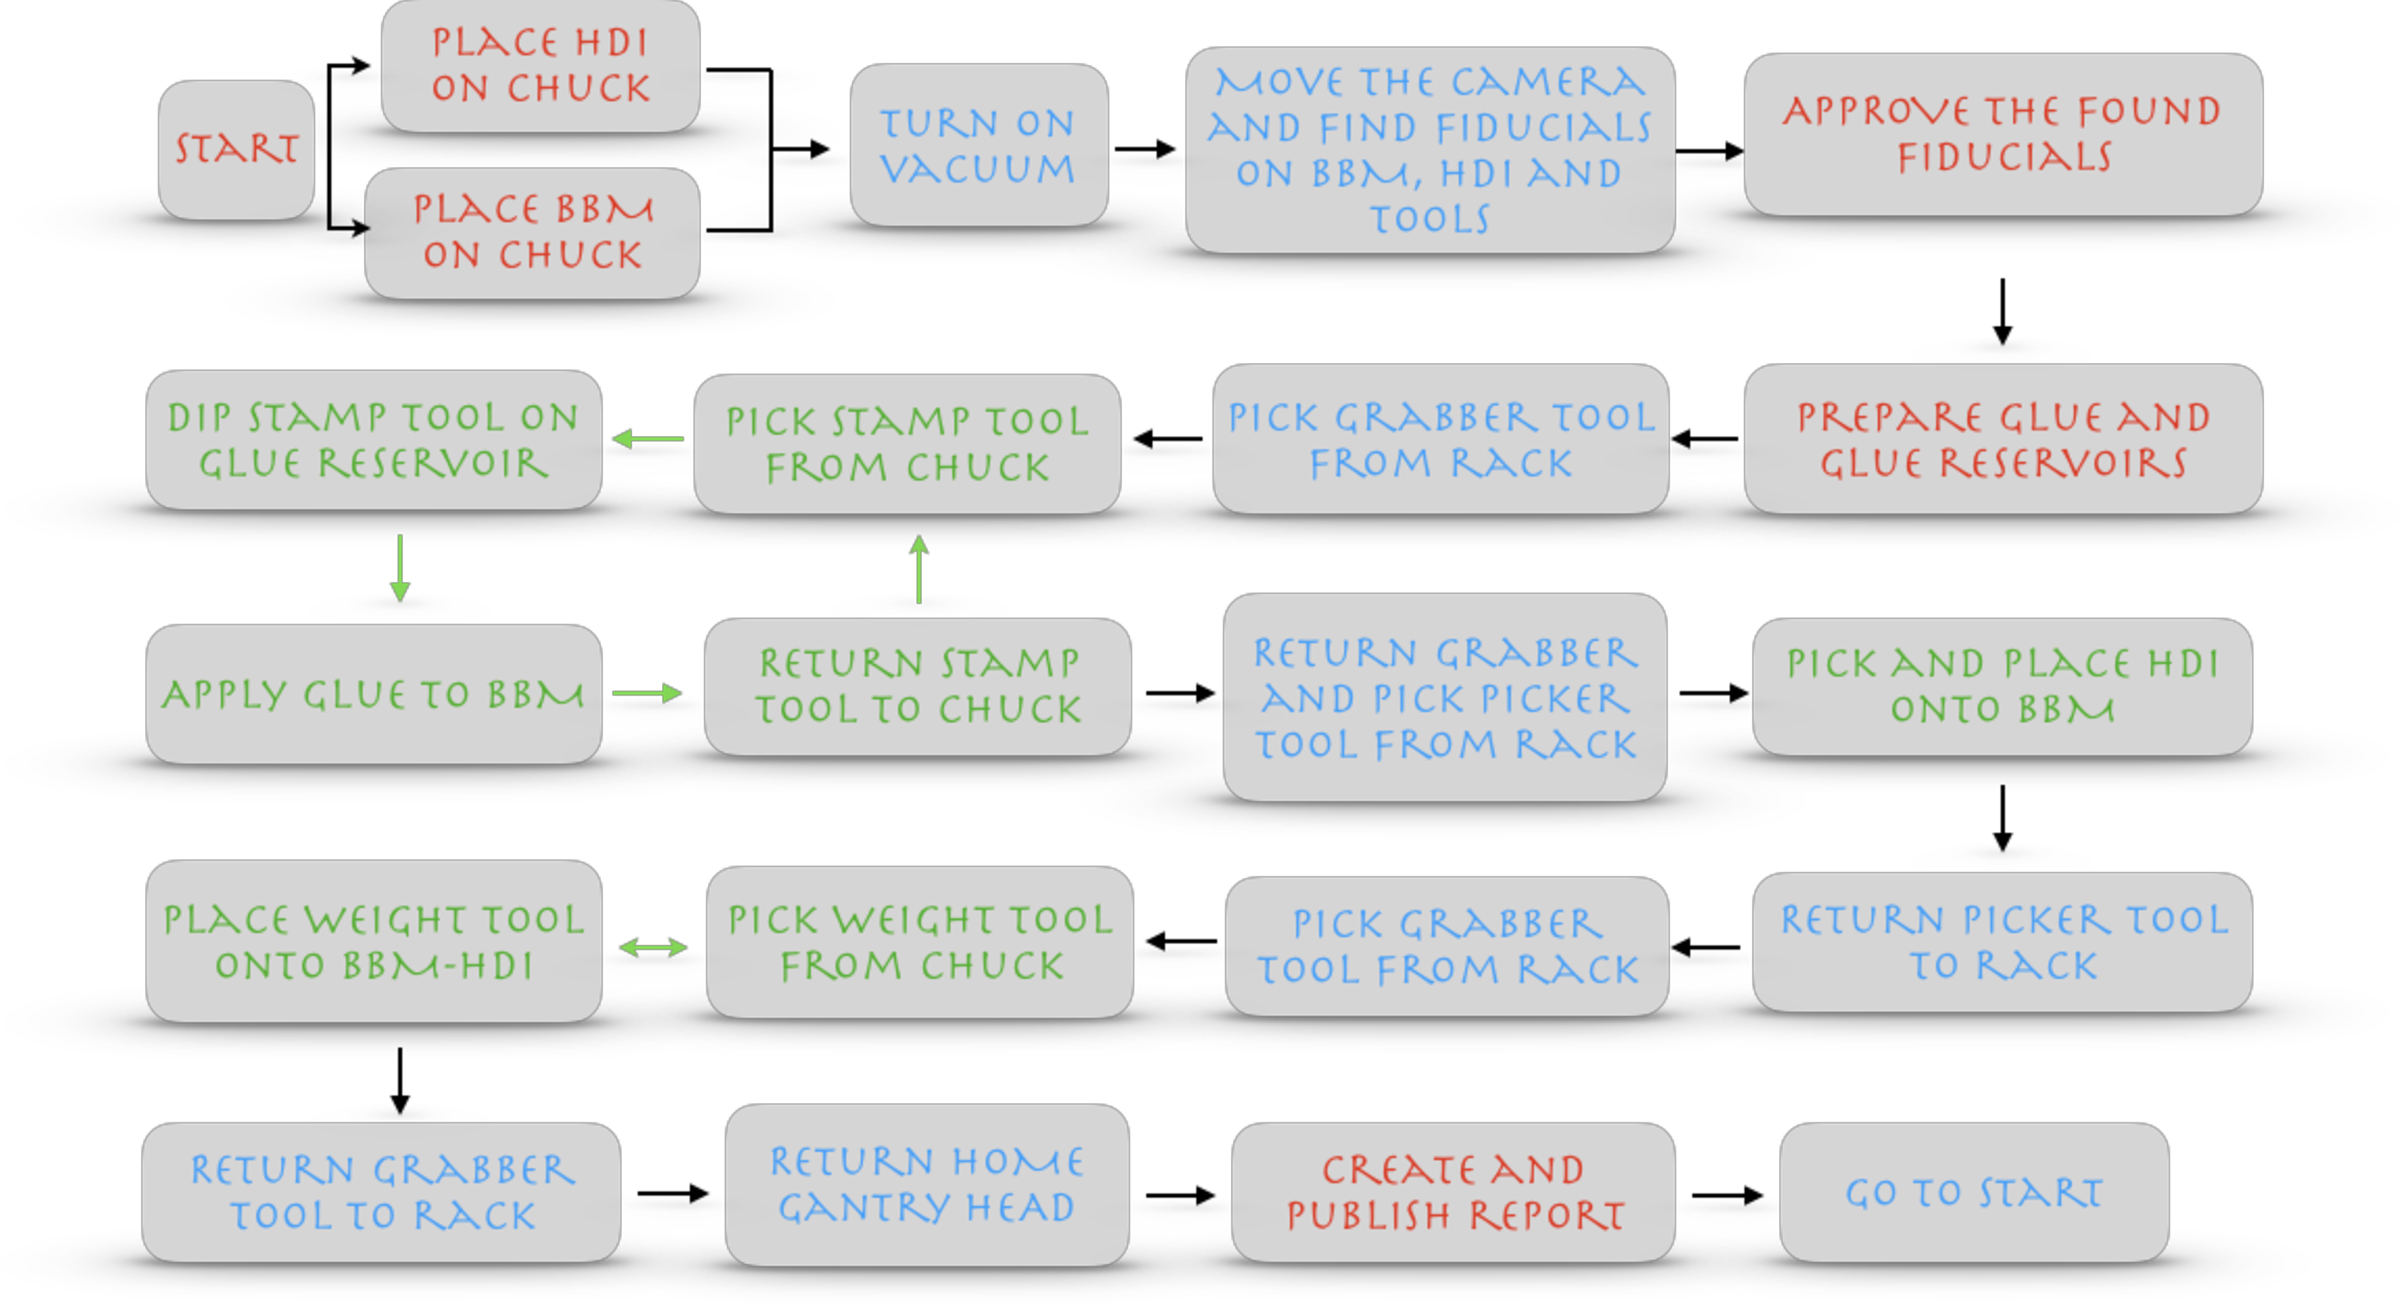
\includegraphics[width=0.9\textwidth]{pixel/glue_workflow2}
    \caption[Gluing routine workflow.]{Gluing routine workflow.}\label{fig:glue_workflow}
  \end{center}
\end{figure}

\begin{landscape}
\begin{figure}[h]
  \begin{center}
    \vspace{-2.5cm}
    \hspace{-1cm}
    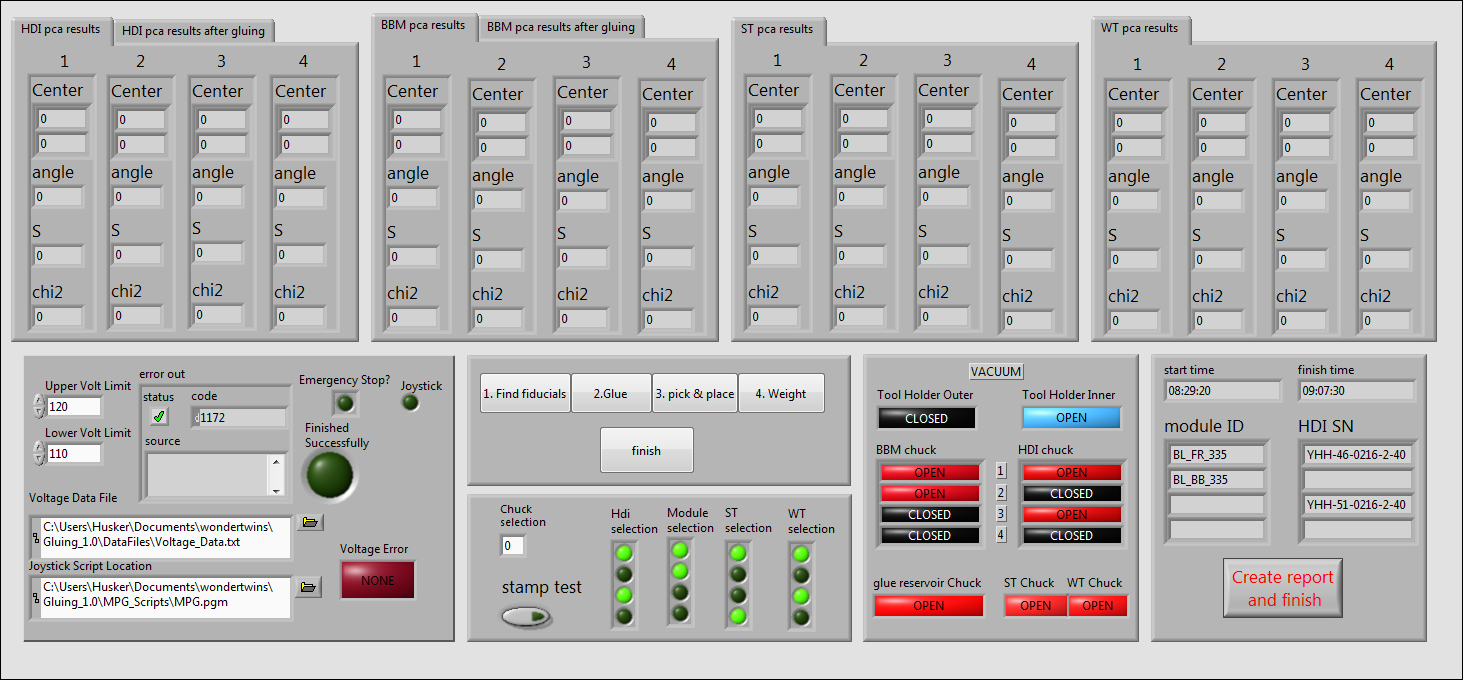
\includegraphics[width=24cm,height=16cm]{pixel/gluing_front_main1.png}
    \caption[Gluing routine LabVIEW front panel]{Gluing routine LabVIEW front panel.}\label{fig:gluing_front_main}
    \vspace{-2cm}
    \hspace{-2cm}
  \end{center}
\end{figure}
\end{landscape}

The gluing routine workflow is shown in Figure\ref{fig:glue_workflow}. The green font represent the steps that are performed more than once in the same session, while the red font represent the steps performed by the operator. It was implemented in a LabVIEW program (\ti{Gluing\_main.vi}) that controls the sequence. The \ti{Main front panel} of the gluing routine, shown in Figure \ref{fig:gluing_front_main}, gathers the most relevant information about the gluing session, while each step in the routine have its dedicated front panel. The module gluing sequence begins by manually placing pre-tested, BBMs, HDIs and tools on their chucks. Once the parts are in place, and the program is run, the BBM and HDI identification information (serial numbers) is collected\footnote{An batch numbering strategy was designed in order to identify the modules intrernally at UNL.} in the first step as well as the configuration of the gantry table, \ie, the BBM/HDI slots and tools to be used so that the vacuum system is properly activated. 

The camera is moved to view, recognize and find the fiducials locations on the BBMs, HDIs and tools. These locations are stored and shown in the Main and \ti{Find fiducials} front panels, so that the operator can identify abnormal values from extreme misalignments and pattern recognition fails; that usually occurs when the plates are not properly placed on the chucks and/or when the fiducials do not appear in the camera field of view. In those cases, a manual fiducial finding option is available. The find fiducial front pannel is shown in Figure \ref{fig:find_fid_front} and a sample of the found fiducials on a HDI and a BBM is shown in Figure \ref{fig:fid_reco} indicating the located center of the fiducial with a green dot.  

\begin{landscape}
\begin{figure}[h]
\begin{center}
    \vspace{-2.9cm}
    \hspace{-1cm}
    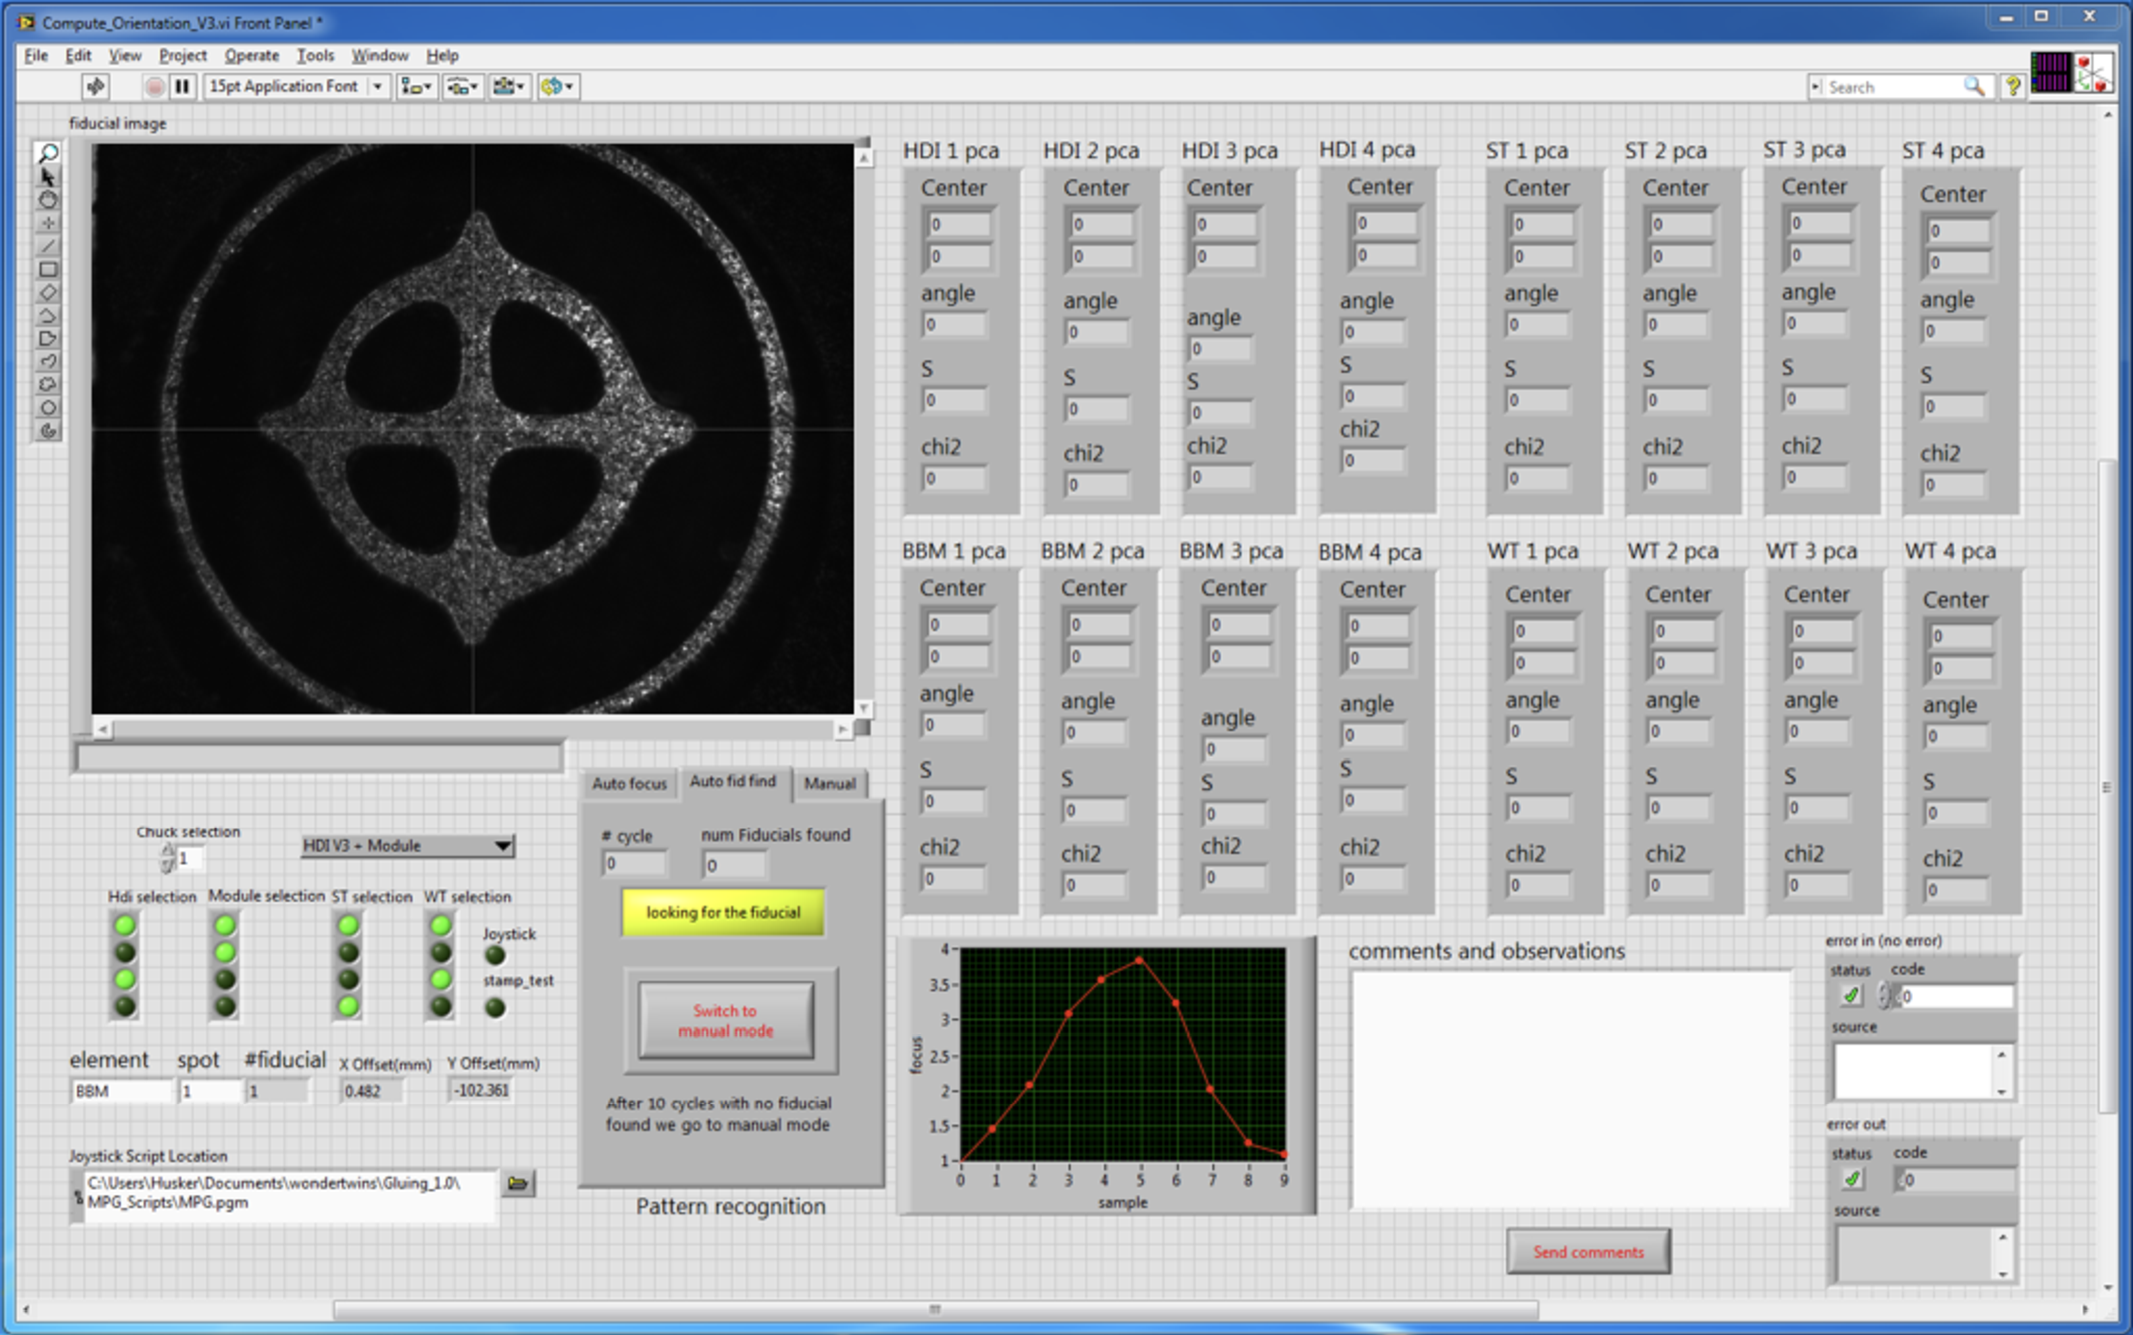
\includegraphics[width=24cm,height=16.5cm]{pixel/find_fid_front}
    \caption[Fiducial finder LabVIEW front panel]{Fiducial finder LabVIEW front panel.}\label{fig:find_fid_front}
    \vspace{-2cm}
    \hspace{-2cm}
\end{center}
\end{figure}
\end{landscape}


\begin{figure}[h]
\begin{center}
 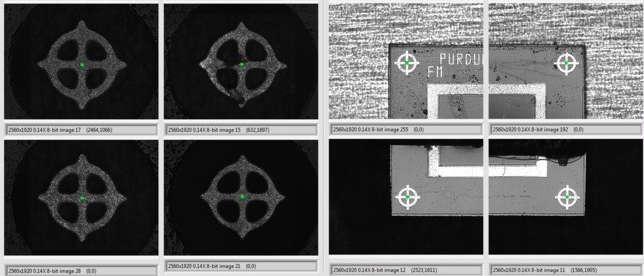
\includegraphics[width=\textwidth]{pixel/fid_reco}
 \caption[Fiducial finder step LabVIEW front panel]{Fiducial finder step LabVIEW front panel.}\label{fig:fid_reco}
\end{center}
\end{figure}

After all the fiducials are identified, the operator has to check them and perform the necessary adjustments. Usually, the glue was prepared in parallel to the fiducial identification, reducing the session time.

The glue application step starts by picking up the grabber tool from the tool rack, and grabbing the stamp tools from their chuck; after dipping the stamp tool in the glue reservoir, the epoxy is dispensed on the BBMs. The procedure is repeated as many times as the number of modules involved in the session, each time using a different stamp tool and a different glue reservoir slot. The step finish by returning the grabber tool to the tool rack. The routine provides full freedom to choose any available combination of stamp tool, glue reservoir slot and BBM; this feature is particularly useful for glue testing and commissioning.









picks up a
vacuum tool from the tool rack to pick-and-place individual HDI onto
sensors (making adjustments based on the actual part locations in the
machine to accurately align and join the components), and returns the
vacuum tool to the tool rack. Module end holders are also aligned and
glued to the modules using custom tooling and the pick-and-place
machine. Following mechanical assembly, HDI are wirebonded to the ROCs
using semi-automated ul- trasonic wirebonding machines. Routine pull
tests of sample wirebonds will be performed for quality control. The
wirebonds will be encapsulated with an elastomeric compound using
semi-automated dispensing equipment. The module assembly sites will
also be responsible for the testing and characterization of the
assembled pixel modules. Modules will be thermally cycled within the
operating temperature range (-20 ◦ C to 20 ◦ C) while monitoring ROC
digital and analog currents. Modules which pass the acceptance
criteria will then be assembled onto the half-disk blades.

The module assembly and testing schedule will depend on the throughput of the pixel modules delivered from the bump-bonding vendors to the module
assembly sites.

In a typical gluing session 4 modules were glued  

\subsection{The Encapsulation stage}

%% \begin{figure}[!h]
%%   \centering
%%   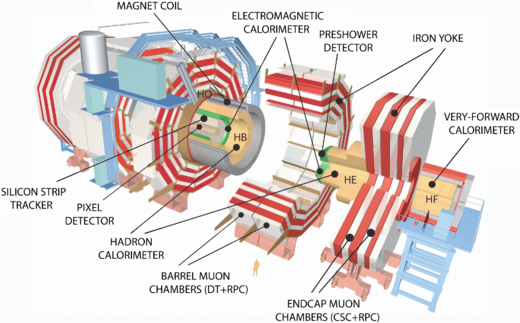
\includegraphics[scale=0.25]{cms}
%%   \caption {ref:  }\label{cms}
%% \end{figure}

\subsection{The FPix module production yields}

%% \begin{figure}[!h]
%%   \centering
%%   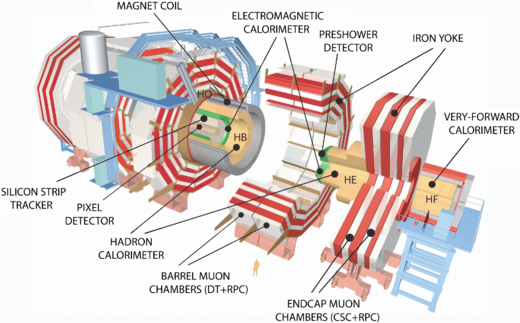
\includegraphics[scale=0.25]{cms}
%%   \caption {ref:  }\label{cms}
%% \end{figure}
